\documentclass[defaultstyle,12pt,master,Helvetica]{01.thesis}
% Helvetica is a similar font to Arial, with small differences.

%% Packages
\typeout{}
\typeout{--------------------------------------------------------------}
\typeout{ +---+ Thesis Template                            }
\typeout{ +---+      Version 2.0, August 2011                         }
\typeout{ +---+  for Instituto Superior Tecnico (IST),                 }
\typeout{ +---+  Universidade Técnica de Lisboa                         }
\typeout{ * Using Thesis Style form Pedro Tomás                                }
\typeout{ * Created to write Dissertations                             }
\typeout{ * Conforms with IST Master Degree format and with most important packages setup        }
\typeout{ * Should conform with IST PhD Degree format (not verified)   }
\typeout{                                                              }
\typeout{ AUTHOR: Miguel Amador and João Marques                                          }
\typeout{                                                              }
\typeout{Important: Use all files in the archive, since this is based in all them. Modify dummy files at wish.                                                              }
\typeout{--------------------------------------------------------------}
\typeout{}

% Defines an additional alphabet... not required in most cases
% ------------------------------------------------------------
% \DeclareMathAlphabet{\mathpzc}{OT1}{pzc}{m}{it}

% PACKAGE babel:
% ---------------
% The 'babel' package may correct some hyphenisation issues of latex. 
% However in most situations it is not required.
\usepackage[english]{babel}

% PACKAGE fontenc:
% -----------------
% chooses T1-fonts and allows correct automatic hyphenation.
%\usepackage[T1]{fontenc}
\usepackage[utf8]{inputenc}

% Package ulem.
\usepackage{ulem} % Allows the use of other text emphatizer commands
\normalem %defines \emph{} to italic, instead of underline. 
\raggedbottom %declaration makes all pages the height of the text on that page. No extra vertical space is added. The \flushbottom declaration makes all text pages the same height, adding extra vertical space when necessary to fill out the page.

% PACKAGE date time:
% -----------------
% Lets you alter the format of the date that \today returns.
\usepackage{datetime}
\newdateformat{todaythesis}{%
\monthname[\THEMONTH]  \THEYEAR}

% PACKAGE latexsym:
% -----------------
% Defines additional latex symbols. May be required for thesis with many math symbols.
\usepackage{latexsym}

% PACKAGE amsmath, amsthm, amssymb, amsfonts:
% -------------------------------------------
% This package is typically required. Among many other things it adds the possibility
% to put symbols in bold by using \boldsymbol (not \mathbf); defines additional 
% fonts and symbols; adds the \eqref command for citing equations. I prefer the style
% "(x.xx)" for referering to an equation than to use "equation x.xx".
\usepackage{amsmath, amsthm, amssymb, amsfonts, amsbsy}

\DeclareMathOperator*{\argmax}{argmax} % thin space, limits underneath in displays

\usepackage{relsize} % allows use of mathlarger

% PACKAGE multirow, colortbl, longtable:
% ---------------------------------------
% These packages are most usefull for advanced tables. The first allows to join rows 
% throuhg the command \multirow which works similarly with the command \multicolumn
% The second package allows to color the table (both foreground and background)
% The third package is only required when tables extend beyond the length of one page;
% with compatibilities with the tabular environment. The last allow the definitions of landscape pages, allowing the use of a different orientation for wider graphics or tables. See package documentation to see the implementation.
\usepackage{multirow}
\usepackage{colortbl}
\usepackage{supertabular}
\usepackage{pdflscape}
% \usepackage{longtable}

% PACKAGE graphics, epsfig, subfigure, caption:
% ---------------------------------------------
% Packages for figures... well you will certainly need these packages, with the exception
% of the 'caption' package. This only allows to define extra caption options.
% Notice that subfigure allows to place figures within figures with its own caption. It
% should be avoided to create an eps file with subfigures. That will mean that you won't be 
% able to reference those subfigures. Instead create an EPS file (the only graphics format supported
% by latex) for each of the subfigures and then use the command \subfigure (see below).
\usepackage{graphics}
\usepackage{graphicx}
\graphicspath{{Figures/}}




\usepackage{epsfig}
%\usepackage[hang,small,bf]{subfigure}
%\usepackage[footnotesize,bf,center]{caption}
\usepackage{dcolumn}
\usepackage{bm}
\usepackage{booktabs}
\usepackage{rotating}
\usepackage{multirow}

\usepackage[font=small,labelfont=bf,textfont=normalfont]{caption}
\usepackage{subcaption}


% PACKAGE algorithmic, algorithm
% ------------------------------
% These packages are required if you need to describe an algorithm.
% \usepackage{algorithmic}
% \usepackage[chapter]{algorithm}

% PACKAGE natbib/cite
% -------------------
% The two packages are not compatible, and you should use one of the two. Notice however that the
% IEEE BiBTeX stylesheet is imcompatible with the natbib package. If using the IEEE format, use the 
% cite package instead
\usepackage[square,numbers,sort&compress]{natbib}
%\usepackage{cite}

% PACKAGE acronyum
% -----------------
% This package is most useful for acronyms. The package guarantees that all acronyms definitions are 
% given at the first usage. IMPORTANT: do not use acronyms in titles/captions; otherwise the definition 
% will appear on the table of contents.
\usepackage[printonlyused]{acronym}
\usepackage[titletoc,title,header]{appendix}
\usepackage[noauto]{chappg}

% PACKAGE extra_functions VER COMO DEVE SER
% -----------------
% My Personal package: defines many
\usepackage{00.extra_functions}


% PACKAGE hyperref
% -----------------
% Set links for references and citations in document
% Some MiKTeX distributions have faulty PDF creators in which case this package will not work correctly
% Long live Linux :D 
% Edit by JM: Indeed!
\usepackage[plainpages=false]{hyperref}
\hypersetup{
             colorlinks=false,
             citecolor=red,
             breaklinks=true,
             bookmarksnumbered=true,
             bookmarksopen=true,
             pdftitle={Thesis Title},
             pdfauthor={Author Name},
             pdfsubject={Master Thesis in Biomedical Engineering},
             pdfcreator={Document Creator Name},
             pdfkeywords={Template, Latex, Thesis}}
\usepackage{float}


%no dashes...
\usepackage[redeflists]{IEEEtrantools}

%different enumerates. Enables: %Roman numbers \begin{enumerate}[label=(\roman*)] (and others)
\usepackage{enumitem}



% Set paragraph counter to alphanumeric mode
\renewcommand{\theparagraph}{\Alph{paragraph}~--}

\newcommand{\figref}[1]{Figure \ref{#1}}
\newcommand{\equationref}[1]{Equation (\ref{#1})}
\newcommand{\tableref}[1]{Table (\ref{#1})}

\newcommand{\textreg}{$\textsuperscript{\textregistered}$}



% Testing packages (gives such a nice formatting of paragraphs!)
\usepackage{parskip}

% Allows the user of \begin{multicols}{2}
\usepackage{multicol} %duh, for multi columns. In itemises, for instance.

% Enable TODO notes in order not to forget certain things...
\usepackage[colorinlistoftodos,prependcaption,textsize=tiny]{todonotes}





%% Page formatting
\hoffset 0in
\voffset 0in

%Alternative set of page geometry
%\oddsidemargin 0.71cm
%\evensidemargin 0.04cm
%\marginparsep 0in
%\topmargin -0.25cm
%\textwidth 15cm
%\textheight 23.5cm

\usepackage[top=2.5cm, bottom=2.5cm, inner=2.9cm, outer=2.5cm]{geometry}

\usepackage{fancyhdr}
\pagestyle{fancy}
\renewcommand{\chaptermark}[1]{\markboth{\thechapter.\ #1}{}}
\renewcommand{\sectionmark}[1]{\markright{\thesection\ #1}}
\fancyhf{} 
%\fancyhead[LE]{\bfseries\nouppercase{\leftmark}}
%\fancyhead[RO]{\bfseries\nouppercase{\rightmark}}
\fancyfoot[C]{\bfseries\small\thepage}
\renewcommand{\headrulewidth}{0.0pt}
\renewcommand{\footrulewidth}{0.0pt}
\addtolength{\headheight}{2pt} % make space for the rule
\fancypagestyle{plain}{% Used in Chapter titles
   \fancyhead{} % get rid of headers
   \renewcommand{\headrulewidth}{0pt} % and the line
   \renewcommand{\footrulewidth}{0pt}
   \fancyfoot[C]{\bfseries\small\thepage}
}

\fancypagestyle{begin}{%
   \fancyhead{}
   \renewcommand{\headrulewidth}{0pt}
   \renewcommand{\footrulewidth}{0pt}
   \fancyfoot[C]{\bfseries\small\thepage}
}
\fancypagestyle{document}{%
	\fancyhf{} 
	\fancyhead[LE]{\bfseries\nouppercase{\leftmark}}
	\fancyhead[RO]{\bfseries\nouppercase{\rightmark}}
	\fancyfoot[C]{\bfseries\small\thepage}
	%\renewcommand{\headrulewidth}{0pt}
	%\renewcommand{\footrulewidth}{0pt}
	\addtolength{\headheight}{2pt} % make space for the rule
}
\fancypagestyle{documentsimple}{%
	\fancyhf{}
	\fancyfoot[C]{\bfseries\small\thepage}
	%\renewcommand{\headrulewidth}{0pt}
	%\renewcommand{\footrulewidth}{0pt}
	\addtolength{\headheight}{2pt} % make space for the rule
}
\setcounter{secnumdepth} {5}
\setcounter{tocdepth} {5}
\renewcommand{\thesubsubsection}{\thesubsection.\Alph{subsubsection}}

%\renewcommand{\subfigtopskip}{0.3 cm}
%\renewcommand{\subfigbottomskip}{0.2 cm}
%\renewcommand{\subfigcapskip}{0.3 cm}
%\renewcommand{\subfigcapmargin}{0.2 cm}

\graphicspath{{Figures/}}

%% Macros 
\newcommand{\defining}[1]{
	\bb{Definition}\hspace{-.2cm} \ii{#1}:
}

\newcommand{\bb}[1]{
	\textbf{#1}
}
 
\newcommand{\ii}[1]{
	\hspace{-1mm}\textit{#1}\hspace{-1mm}
}

\newcommand{\ul}[1]{
	\uline{#1}
}

\newcommand{\tdegv}[0]{
	\hspace{-1.5mm}°
}
\newcommand{\tdeg}[0]{
	\hspace{-1.5mm}\textdegree \space
}

\newcommand{\image}[4]{
	\begin{center}

		\includegraphics[scale = #4]{#1}
    	\captionsetup{type=figure} 
   		\caption{#2}			
        \label{#3}
        
    \end{center}
}

\newcommand{\imagecapcontrol}[5]{
	\begin{center}

		\includegraphics[scale = #4]{#1}
    	\captionsetup{type=figure} 
		\vspace{#5}   
		\caption{#2}			
        \label{#3}
        
    \end{center}
}


%possible to use: \ifthenelse{\isempty{#1}}{#1}{default value for #1} for optional arguments

\newcommand{\imagenolabel}[3]{
	\begin{center}

		\includegraphics[scale = #3]{#1}
		\captionsetup{type=figure} 
		\caption{#2}			
		
	\end{center}
}



%to make an \hrule have the ruler in the middle of the line. Use \Vhrulefill
\def\Vhrulefill{\leavevmode\leaders\hrule height 0.7ex depth \dimexpr0.4pt-0.7ex\hfill\kern0pt}


\newcommand{\quickimage}[2]{
	\begin{center}
		\includegraphics[scale = #2]{#1}
    \end{center}
}

\newcommand{\quickimagesidebyside}[4]{
	\begin{figure}[!h]
		\centering
		\begin{subfigure}{0.5\textwidth}
		  \centering
		  \includegraphics[width=#2\linewidth]{#1}
		\end{subfigure}%
		\begin{subfigure}{0.5\textwidth}
		  \centering
		  \includegraphics[width=#4\linewidth]{#3}
		\end{subfigure}
	\end{figure}
}

%Note: you can't use numbers on definitions

%One label on the overall figure
\newcommand{\imagesidebysideonelabel}[8]{
	\begin{figure}[!h]
		\centering
		\begin{subfigure}{0.5\textwidth}
		  \imagenolabel{#1}{#2}{#3}
		\end{subfigure}%
		\begin{subfigure}{0.5\textwidth}
		  \imagenolabel{#4}{#5}{#6}
		\end{subfigure}
		\caption{#7}
		\label{#8}
	\end{figure}
}


%Labels on both subfigures
\newcommand{\imagesidebysidetwolabels}[9]{
	\begin{figure}[!h]
		\centering
		\begin{subfigure}{0.5\textwidth}
		  \image{#1}{#2}{#3}{#4}
		\end{subfigure}%
		\begin{subfigure}{0.5\textwidth}
		  \image{#5}{#6}{#7}{#8}
		\end{subfigure}
		\caption{#9}
	\end{figure}
}


\newcommand{\imagesidebysidenosubfigure}[8]{
	\begin{figure}
		\centering
		\begin{minipage}{.5\textwidth}
			\image{#1}{#2}{#3}{#4}
		\end{minipage}%
		\begin{minipage}{.5\textwidth}
			\image{#5}{#6}{#7}{#8}
		\end{minipage}
	\end{figure}
}




% Game has changed! More than 9 Arguments now!!!

% LIKE THIS:
\newcommand\foo[9]{
    \def\tempa{#1}
    \def\tempb{#2}
    \def\tempc{#3}
    \def\tempd{#4}
    \def\tempe{#5}
    \def\tempf{#6}
    \def\tempg{#7}
    \def\temph{#8}
    \def\tempi{#9}
    \foocontinued
}

\newcommand\foocontinued[7]{%
	% Do whatever you want with your 9+7 arguments here.
	\tempa 
	\tempb
	This is the 10th argument: #1
	This is the 16th argument: #7
}

% How to use: you now use \foo{1}{2}...{9}{10} or until 18, and keep doing it.
% NOTE 1: you have to call \foo at least with 10 arguments, even if \foocontinued can take more, the others will be considered to be empty. Call: \foo{1}{2}{3}{4}{5}{6}{7}{8}{9}{10} to test.
% NOTE 2: that all variables can only be accessed in the last command.
% NOTE 3: latex variables can't have numbers... so 'tempa' is the best we can do.

\newcommand{\imagesidebysidecomplete}[9]{
	\def\tempa{#1}
    \def\tempb{#2}
    \def\tempc{#3}
    \def\tempd{#4}
    \def\tempe{#5}
    \def\tempf{#6}
    \def\tempg{#7}
    \def\temph{#8}
    \def\tempi{#9}
    \imagesidebysidecompletecontinued
}

\newcommand{\imagesidebysidecompletecontinued}[3]{
	\begin{figure}[!h]
		\centering
		\begin{subfigure}{#2\textwidth}
		  \image{\tempa}{\tempb}{\tempc}{\tempd}
		\end{subfigure}%
		\begin{subfigure}{#3\textwidth}
		  \image{\tempe}{\tempf}{\tempg}{\temph}
		\end{subfigure}
		\caption{\tempi}
		\label{#1}
	\end{figure}
}





\newcommand{\threeimagessidebyside}[9]{
	\def\tempa{#1}
    \def\tempb{#2}
    \def\tempc{#3}
    \def\tempd{#4}
    \def\tempe{#5}
    \def\tempf{#6}
    \def\tempg{#7}
    \def\temph{#8}
    \def\tempi{#9}
    \threeimagessidebysidecontinued
}

\newcommand{\threeimagessidebysidecontinued}[9]{
\begin{figure}[h]
    \centering
    \begin{subfigure}[b]{#6\textwidth}
        \image{\tempa}{\tempb}{\tempc}{\tempd}
    \end{subfigure}
     %add desired spacing between images, e. g. ~, \quad, \qquad, \hfill etc. 
      %(or a blank line to force the subfigure onto a new line)
	\begin{subfigure}[b]{#7\textwidth}
		\image{\tempe}{\tempf}{\tempg}{\temph}
    \end{subfigure}
     %add desired spacing between images, e. g. ~, \quad, \qquad, \hfill etc. 
    %(or a blank line to force the subfigure onto a new line)
	\begin{subfigure}[b]{#8\textwidth}
		\image{\tempi}{#1}{#2}{#3}
    \end{subfigure}
    \caption{#4}\label{#5}
\end{figure}
}


% This is amazing: https://tex.stackexchange.com/questions/8351/what-do-makeatletter-and-makeatother-do

% \subalign method to align indices in the summatories
\makeatletter
\newcommand{\subalign}[1]{%
  \vcenter{%
    \Let@ \restore@math@cr \default@tag
    \baselineskip\fontdimen10 \scriptfont\tw@
    \advance\baselineskip\fontdimen12 \scriptfont\tw@
    \lineskip\thr@@\fontdimen8 \scriptfont\thr@@
    \lineskiplimit\lineskip
    \ialign{\hfil$\m@th\scriptstyle##$&$\m@th\scriptstyle{}##$\hfil\crcr
      #1\crcr
    }%
  }%
}
\makeatother

%-----------------------------------------------------------
%-----------------------------------------------------------
\begin{document}

%bibliography set (no dashed names when repeated)
\bstctlcite{IEEEexample:BSTcontrol}

 

\pagestyle{begin}


\hypersetup{hidelinks} % to hide (not underline) links from then on.

%\setcounter{page}{1} \pagenumbering{Alph}

% Add PDF bookmark 
\pdfbookmark[0]{Title}{Title}

\thispagestyle{empty}
\begin{flushleft} ~\\ \vspace{-12mm} \hspace{-12mm}  
\includegraphics[width=50mm]{Cover/istnewlogo} 
\vspace{10mm}
%~\\ \vspace{50mm} % gr�ficos
\\ \begin{center} 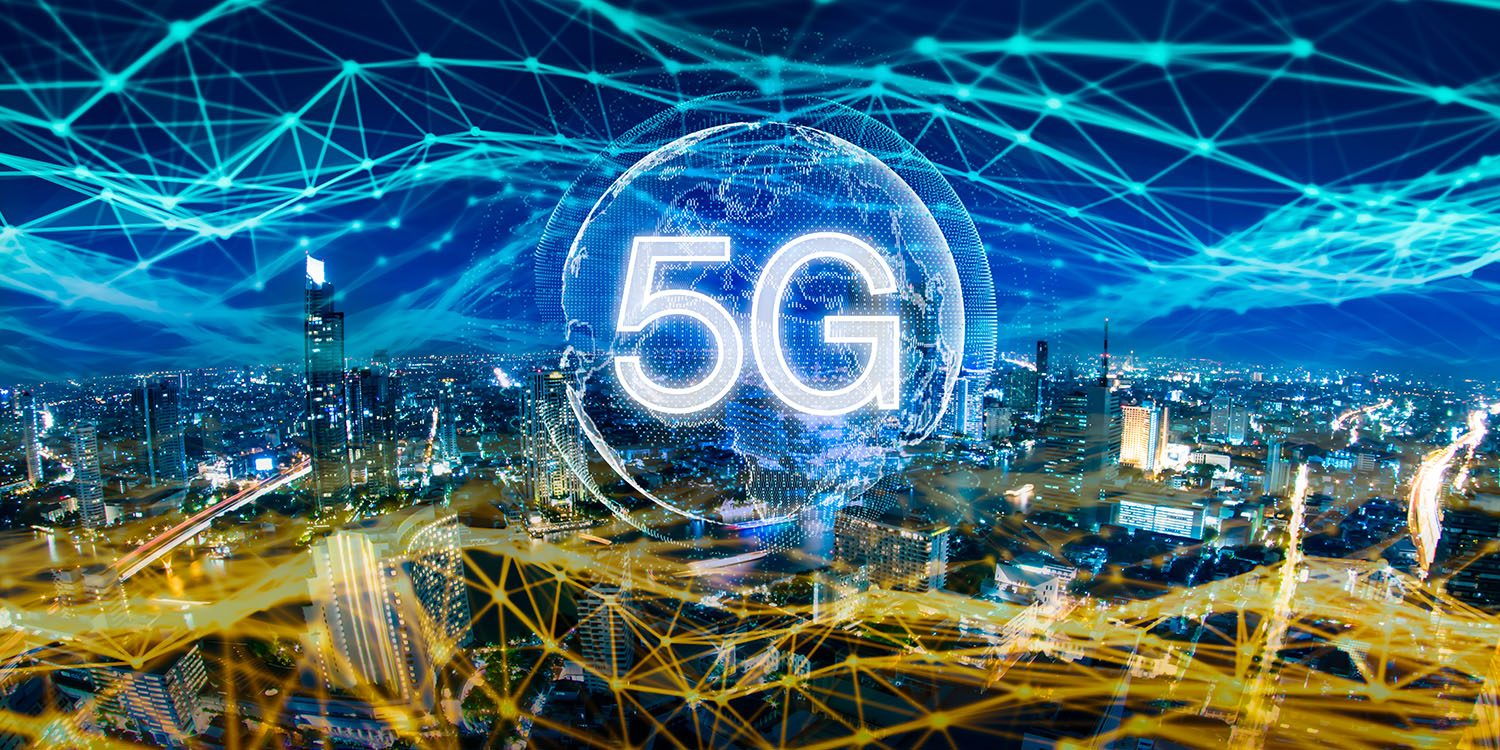
\includegraphics[height=50mm]{Cover/5G}  \end{center} % graficos
 \vspace{5mm}
\centering
\LARGE \textbf{Performance Modelling for \\Social VR Conference Applications in\\Beyond-5G Radio Access Networks}
\\ \vspace{15mm}
%\Large Preparation
%\\ \vspace{15mm}
\Large \textbf{Jo{\~a}o Alberto Janeiro Horta de Morais} \\
\vspace{15mm}
\large Thesis to obtain the Master of Science Degree in
\\ \vspace{2mm}
\LARGE \textbf{Electrical and Computer Engineering}
\\ \vspace{10mm}
\fontsize{14pt}{\baselineskip} \selectfont 
\begin{tabular}{rl}
    Supervisors: & Prof. Ant{\'o}nio Jos{\'e} Castelo Branco Rodrigues \\
    & Prof. Remco Litjens \\
\end{tabular}

\vspace{8mm}
\Large \textbf{Examination Committee}\\ 
\vspace{4mm}
\fontsize{12pt}{\baselineskip} \selectfont 
\begin{tabular}{rl}
    Chairperson: & Prof. Jos{\'e} Eduardo Charters Ribeiro da Cunha Sanguino \\
    Supervisor: & Prof. Ant{\'o}nio Jos{\'e} Castelo Branco Rodrigues \\
    Members of the Committee: & Prof. Ant{\'o}nio Francisco Bucho Cercas \\
\end{tabular}


%\large Prof. Jos{\'e} Eduardo Charters Ribeiro da Cunha Sanguino \\
%\large Chairperson:~Prof.~Jos{\'e}~Eduardo~Charters~Ribeiro~da~Cunha~Sanguino \\
%\large Supervisor: Prof. \\
%\large Co-Supervisor:  Prof .\\
%\large Members of the Committee: \\
\vspace{3mm} %%%%%%%%%%%%%%%%%%5 Add space!

%\Large \textbf{\todaythesis\today} \\
\Large \textbf{February 2021} \\
\let\thepage\relax
\end{flushleft}
\pagebreak


\clearpage
% Since I am using double sided pages, the second page should be white.
% Remember that when delivering the dissertation, IST requires for the cover to appear twice.

\thispagestyle{empty}
\cleardoublepage

\setcounter{page}{1} \pagenumbering{roman}

\baselineskip 18pt % line spacing: -12pt for single spacing
                   %               -18pt for 1 1/2 spacing
                   %               -24pt for double spacingnts}
\chapter*{Declaration}

I declare that this document is an original work of my own authorship and that 
it fulfils all the requirements of the Code of Conduct and Good Practices of the 
Universidade de Lisboa.
\clearpage
\thispagestyle{empty}
\cleardoublepage

   
\begin{center}
    \LARGE \bb{Foreword}
\end{center}

\vspace{1cm}

The research presented in this document was conducted in TNO as part of a project called ‘Empowered Edge’, in the first year of a large research programme on Social-Extended Reality. Naturally, the research will continue and one of the main concerns throughout of this project has been guaranteeing flexibility 


to use this simulator and several directions described in the future work section will be pursued.


This thesis




% the direction this is taking...

% this allowed one internship and 2 MSc thesis

% working on this project also facilitated the process of creating two patents for other projects within TNO.
``C'mon, thousands of hours and I can only pick one quote? Do you think I write stuff like this every Tuesday? I'm choosing as many as I want!'' - Me.


Distorting what Isaac Newton said:

``We can see further by standing upon the shoulders of giants.''
%A thank you to the people that worry about knowledge transfer

Vapnik principle:
``When trying to solve a problem, we should not solve a more difficult problem as an intermediate step.''
%to say thank you for all the advice from my coordinators that helped simplifying the problem when I was trying to solve harder ones as intermediate steps...

Feynman
``We must be careful not to believe things simply because we want them to be true''
It continues to: ``No one can fool you as easily as you can fool yourself''

Alasdair Gray
``Work as if you live in the early days of a better nation''


``Premature optimisation is the root of all evil...''- Donald Knuth - ``... (or at least most of it) in programming.''


``You can never cross the ocean unless you have the courage to lose sight of the shore.'' - Cristóvão Colombo (Christopher Columbus)


``Do things on your own terms, do things in your own time, do things for yourselves, and give everything away.'' - Jacob Collier



\ul{(ideas for quotes. They should be at the bottom)}


\thispagestyle{empty}
\hbox{} \vfill
\begin{flushright}
\small \textit{\textbf{Anyone who has never made a mistake has never tried anything new.}}
\\ \vspace{2mm}  
\scriptsize Albert Einstein
\end{flushright}

\clearpage
\thispagestyle{empty}
\cleardoublepage


\pdfbookmark{Acknowledgments}{Acknowledgments}
\begin{acknowledgments} 

I would like to thank the Academy, bla bla bla..
\begin{comment}

%To Miguel Amador, for the Thesis Template. Also, more generally, to everyone that strives to transmit knowledge, share their work and allow their findings to be used as a base - to every professor, online lecturer, fellow colleague and everyone curious enough to go extensive lengths while worrying its work can be used by others and built upon.

My professor in Portugal, António Rodrigues, who helped unconditionally when it was needed, sometimes through the \ii{horse's door}, and allowed for a lot of freedom.

Since this marks the end of five years of studying, and I'm not planning on writing another of these any time soon, I should thank who shape my path along the way.
Some professors... Mário Silveirinha, António Topa, ...

And, fortunately, to too many friends to list, with whom I hope not to loose too much contact.



Concrete content contributions to this document:
- Maria for the MCS curves;
- Onno, Yohan, Manolis and Remco for the MIESM figure;
- 
- Remco for some figures;
- Remco and Sjors for reviewing;


HUGE thank you to TNO: invested in hardware necessary to deal with huge amounts of data, letting me using their Cloud for computations, ... and much more



% This is final:

To my advisory team in Hans, Remco and Sjors, for crucial reviews, for more than 50 meetings, more countless emails, and for any physical or virtual interaction. I always learned something. In particular Remco...

To the radio people. To other incredibly nice and no less important 


Niels, ... fortunately, way too many to count! There are more than about 90 people in the department. 

Among these people... Lucia ....

To Lucia (yes, again!), Eduardo, Mike, Dinho, Rosa and others that were the scarce but essential training partners I had during the pandemic.


To my good friends Afonso and Bernardo. For amazing talks that provided the perfect escape after a long day. For accountability with the studies. For the countless rides back and forth when I could not walk. But especially for proving over more than ten years that real friendship does not look at gender, race or social class. Although we are all middle class, white and male... This was a joke. Thanks for always reminding of what fun is.

And to my parents. For always doing their best to give me everything I could need. 


\end{comment}
\end{acknowledgments}
\clearpage
\thispagestyle{empty}
\cleardoublepage
\begin{abstract}

    One of the most challenging applications targeted by evolving (beyond-)5G technology is virtual reality (VR). Particularly, ‘Social VR’ applications provide a fully immersive experience and sense of togetherness to users residing at different locations. To support such applications the network must deal with enormous traffic demands, while keeping end-to-end latencies low. Moreover, the radio access network must deal with the volatility and vulnerability of mm-wave radio channels, where even small movements of the users may cause line-of-sight blockage, causing severe throughput reductions and hence Quality of Experience (QoE) degradation or even lead to loss of connectivity. In this work we present and validate an integral modelling approach for feasibility assessment and performance optimisation of the radio access network for Social VR applications in indoor office scenarios. Such modelling enables us to determine the performance impact of e.g. ‘natural’ human behaviour, the positions and configurations of the antennas and different resource management strategies. Insights into these issues are a prerequisite for setting up guidelines for network deployment and configuration as well as for the development of (potentially AI/ML-based) methods for dynamic resource management and tuning of radio access parameters to best support Social VR applications.
    
\end{abstract}
\begin{keywords}
Modelling, Virtual Reality, 5G, Radio Access Networks, Wireless Communications
\end{keywords}
\clearpage
\thispagestyle{empty}
\cleardoublepage
\begin{resumo}

O objectivo deste trabalho ... (Portugu�s)

\end{resumo}            
\begin{palavraschave}
Modelação, Realidade Virtual, 5G, Redes de Acesso Rádio, Communicações Móveis
\end{palavraschave}
\clearpage
\thispagestyle{empty}
\cleardoublepage  
% This is required for the fancy chapters
\dominitoc
\dominilof
\dominilot

%%%%%%%%%%%%%%%%%%%%%%%%%%%%%%%%%%%%%%%%%%%%%%%%%%%%%%%%%%%%%%%%%%%%%%
% List of contents
%\renewcommand{\baselinestretch}{1}
\pdfbookmark[0]{Index}{index}
\pdfbookmark[1]{Contents}{toc}
\tableofcontents
% \contentsline{chapter}{References}{\pageref{bib}}
\clearpage
\thispagestyle{empty}
\cleardoublepage
%\renewcommand{\baselinestretch}{1.5}
%%%%%%%%%%%%%%%%%%%%%%%%%%%%%%%%%%%%%%%%%%%%%%%%%%%%%%%%%%%%%%%%%%%%%%
% List of figures
\pdfbookmark[1]{List of Figures}{lof}
\listoffigures
\clearpage
\thispagestyle{empty}
\cleardoublepage

%%%%%%%%%%%%%%%%%%%%%%%%%%%%%%%%%%%%%%%%%%%%%%%%%%%%%%%%%%%%%%%%%%%%%%
% List of tables
\pdfbookmark[1]{List of Tables}{lot}
\listoftables
\clearpage
\thispagestyle{empty}
\cleardoublepage

% %%%%%%%%%%%%%%%%%%%%%%%%%%%%%%%%%%%%%%%%%%%%%%%%%%%%%%%%%%%%%%%%%%%%%%
% % List of algorithms
% Requires packages algorithmic, algorithm
% \pdfbookmark[1]{List of Algorithms}{loa}
% \listofalgorithms
% \cleardoublepage
% %%%%%%%%%%%%%%%%%%%%%%%%%%%%%%%%%%%%%%%%%%%%%%%%%%%%%%%%%%%%%%%%%%%%%%
 % List of acronyms
\pdfbookmark[1]{List of Abbreviations}{loac}

\chapter*{List of Abbreviations}

\acresetall %for resetting acronyms... CHECK THE CAPTIONS NAMES!! MAYBE acs is required there.

% See more at http://staff.science.uva.nl/~polko/HOWTO/LATEX/acronym.html

%these need to be put in order eventually
\begin{acronym}[MU-MIMO] %PUT HERE the longest acronym used for proper alignment
\acro{acro}{Dummy Acronym}

% #
\acro{3GPP}{3rd Generation Partnership Project}
\acro{3G}{3rd Generation}
\acro{4G}{4th Generation}
\acro{5G}{5th Generation}
\acro{5GC}{5th Generation Core}
\acro{5GI}{5G QoS Identifier}

% A

\acro{AAA}{Authentication, Authorisation, and Accounting}
\acro{ACK}{Acknowledgement}
\acro{ADC}{Analog-to-Digital Converter}
\acro{AE}{Antenna Element}
\acro{AFD}{Average Fade Duration}
\acro{AGCH}{Access Grant Channel}
\acro{AI}{Artificial Intelligence}
\acro{AM}{Acknowledged Module}
\acro{AMC}{Adaptive Modulation and Coding}
\acro{AMF}{Access and Mobility Management Function}
\acro{AMPS}{Advanced Mobile Phone System}
\acro{AN}{Access Network}
\acro{ANACOM}{Autoridade Nacional de Comunicações}
\acro{ANSI}{American National Standards Institute}
\acro{AR}{Augmented Reality}
\acro{ARQ}{Automatic Repeat Query}
\acro{AS}{Access Stratum}
\acro{AP}{Access Point}
\acro{API}{Application Programming Interface}
\acro{AuC}{Authentication Centre}
\acro{AWGN}{Additive White Gaussian Noise}



% B
\acro{BB}{Base Band}
\acro{BCCH}{Broadcast Control Channel}
\acro{BCH}{Broadcast Channel}
\acro{BER}{Bit Error Ratio}
\acro{BLER}{Block Error Rate}
\acro{BS}{Base Station}
\acro{BPF}{Band Pass Filter}
\acro{BPSK}{Binary Phase Shift Keying}
\acro{BSC}{Base Station Controller}
\acro{BSS}{Base Station Subsystem}
\acro{BTS}{Base Transceiver Station}
\acro{BU}{Bad Urban}

% C
\acro{CA}{Carrier Aggregation}
\acro{CCCH}{Common Control Channel}
\acro{CCH}{Control Channel}
\acro{CDF}{Cumulative Distribution Function}
\acro{CDMA}{Code Division Multiple Access}
\acro{CENELEC}{Comité Européen de Normalisation Electrotechnique}
\acro{CN}{Core Network}
\acro{CodS}{Coding Scheme}
\acro{CoMP}{Coordinated Multipoint}
\acro{COST}{European Co-operation in the Field of Scientific and Technical Research}
\acro{CP}{Cyclic Prefix}
\acro{CPCH}{Common Packet Channel}
\acro{CPU}{Central Processing Unit}
\acro{CQI}{Channel Quality Indicator}
\acro{CRC}{Cyclic Redundancy Check}
\acro{CS}{Circuit Switch}
\acro{CSI}{Channel State Information}
\acro{CSI-RS}{Channel State Information - Refference Signal}
\acro{CTCH}{Common Traffic Channel}

% D
\acro{D2D}{Device-to-device}
\acro{D-AMPS}{Digital-Advanced Mobile Phone System}
\acro{DAC}{Digital-to-Analog Converter}
\acro{DCCH}{Dedicated Control Channel}
\acro{DCH}{Dedicated Channel}
\acro{DECT}{Digital Enhanced Cordless Telecommunications}
\acro{DL}{Downlink}
\acro{DN}{Data Network}
\acro{DNN}{Deep Neural Network}
\acro{DPCCH}{Dedicated Physical Control Channel}
\acro{DPDCH}{Dedicated Physical Data Channel}
\acro{DQPSK}{Differential Quadrature Phase Shift Keying}
\acro{DRB}{Data Radio Bearer}
\acro{DSCH}{Dedicated Shared Channel}
\acro{DTCH}{Dedicated Traffic Channel}

% E
\acro{EBF}{Explicit Beamforming}
\acro{EGC}{Equal Gain Combining}
\acro{EGDE}{Enhanced Data rates for GSM Evolution}
\acro{EHD}{Environmental Health Division}
\acro{EHF}{Extremely High Frequency}
\acro{EIRP}{Equivalent Isotropic Radiated Power}
\acro{eMBB}{extreme Mobile Broadband}
\acro{eNB}{evolved Node B}
\acro{EPC}{Evolved Packet Core}
\acro{ERPd}{Effective Radiated Power by half wavelength dipole}
\acro{ESN}{Echo State Network}
\acro{E-UTRA}{Evolved-UMTS Terrestrial Radio Access}
\acro{E-UTRAN}{Evolved-UMTS Terrestrial Radio Access Network}
\acro{EXP/PF}{Exponential/Proportional Fair}

% F
\acro{FACCH}{Fast Associated Control Channel}
\acro{FACH}{Forward Access Channel}
\acro{FCCH}{Frequency Correction Channel}
\acro{FDD}{Frequency Division Duplex}
\acro{FDM}{Frequency-Division Multiplexing}
\acro{FDMA}{Frequency-Division Multiple Access}
\acro{FEC}{Foward Error Correction}
\acro{FIFO}{First In First Out}
\acro{FM}{Frequency Modulation}
\acro{FNBW}{First Null Beam Width}
\acro{FOV}{Field Of View}
\acro{FR}{Frequency Range}
\acro{FPS}{Frames Per second}
\acro{FTP}{File Transfer Protocol}
\acro{FWA}{Fixed Wireless Access}


% G
\acro{GB}{GigaBytes}
\acro{GBR}{Guaranteed Bit Rate}
\acro{GGSN}{Gateway GPRS Support Node}
\acro{GMSK}{Gaussian Minimum Shift Keying}
\acro{gNB}{Next Generation Node B}
\acro{GoB}{Grid of Beams}
\acro{GoP}{Group of Pictures}
\acro{GoS}{Grade of Service}
\acro{GPRS}{General Packet Radio System}
\acro{GPT-U}{GPRS Tunneling Protocol User plane}
\acro{GSM}{Global System for Mobile Communications}

% H
\acro{HARQ}{Hybrid Automatic Repeat Request}
\acro{HEVC}{High Efficiency Video Coding}
\acro{HF}{High Frequency}
\acro{HLR}{Home Location Register}
\acro{HMD}{Head Mounted Display}
\acro{HO}{Handover}
\acro{HPBW}{Half-Power Beam Width}
\acro{HSCSD}{High Speed Circuit Switched Data}
\acro{HSDPA}{High-Speed Downlink Packet Access}
\acro{HSPA}{High-Speed Packet Access}
\acro{HSS}{Home Subscriber Server}
\acro{HSUPA}{High-Speed Uplink Packet Access}
\acro{HT}{Hilly Terrain}
\acro{HTTP}{Hypertext Transfer Protocol}

% I
\acro{IBF}{Implicit Beamforming}
\acro{ICIC}{Inter-Cell Interference Coordination}
\acro{ICNIRP}{International Commission on Non-Ionising Radiation Protection}
\acro{IEEE}{Institute of Electrical and Electronics Engineers}
\acro{IF}{Intermediate Frequency}
\acro{IMS}{IP Multimedia Subsystem}
\acro{IP}{Internet Protocol}
\acro{IQ}{In-phase and Quadrature}
\acro{IRPA}{International Radiation Protection Association}
\acro{IS-94}{Interim Standard 94}
\acro{ISDN}{Integrated Services Digital Network}
\acro{ISI}{Inter-Symbol Interference}
\acro{ITU}{International Telecommunications Union}
\acro{ITU-R}{International Telecommunications Union – Radio sector}

% J

% K
\acro{KPI}{Key Performance Indicator}

% L
\acro{L1}{Layer 1}
\acro{L2}{Layer 2}
\acro{L3}{Layer 3}
\acro{L4}{Layer 4}
\acro{L5}{Layer 5}
\acro{LAN}{Local Area Network}
\acro{LBT}{Listen-before-talk}
\acro{LCR}{Level Crossing Rate}
\acro{LF}{Low Frequency}
\acro{LIFO}{Last In First Out}
\acro{LLC}{Link Layer Control}
\acro{LMS}{Least Mean Squares}
\acro{LoS}{Line-of-Sight}
\acro{LTE}{Long-Term Evolution}

% M
\acro{MAC}{Medium Access Control}
\acro{MCS}{Modulation and Coding Scheme}
\acro{MCU}{Multi-point Control Unit}
\acro{MF}{Medium Frequency}
\acro{MIMO}{Multiple-Input Multiple-Output}
\acro{MIESM}{Mutual Information Effective SINR Mapping}
\acro{M-LWDF}{Maximum-Largest Weighted Delay First}
\acro{MME}{Mobility Management Entity}
\acro{MMSE}{Minimum Mean-Square Error}
\acro{mMTC}{massive Machine-Type Communications}
\acro{mmWave}{Millimetre Wave}
\acro{ML}{Machine Learning}
\acro{MR}{Maximum Ratio}
\acro{MRC}{Maximum Ratio Combining}
\acro{MRT}{Maximum Ratio Trasmission}
\acro{MSC}{Mobile Switching Centre}
\acro{MTP}{Motion-to-photon}
\acro{MU-MIMO}{Multi-user MIMO}

% N
\acro{NAMTS}{NEC Advance Mobile Telephone System}
\acro{NAS}{Non-Access Stratum}
\acro{NB}{Node B}
\acro{NEC}{Nippon Electric Company}
\acro{NLoS}{Non-Line-of-Sight}
\acro{NMT}{Nordic Mobile Telephone}
\acro{NN}{Neural Network}
\acro{nGBR}{Non-Guaranteed Bit Rate}
\acro{NG}{Next Generation}
\acro{ng-eNB}{Next Generation evolved Node B}
\acro{NG-AP}{Next Generation Application Protocol}
\acro{NG-RAN}{Next Generation Radio Access Network}
\acro{NR}{New Radio}





% O
\acro{OFDM}{Orthogonal Frequency Division Multiplexing}
\acro{OFDMA}{Orthogonal Frequency Division Multiple Access}
\acro{OLLA}{Outer Loop Link Adaptation}
\acro{OSI}{Open Systems Interconnection}
\acro{OVSF}{Orthogonal Variable Spreading Factor}

% P
\acro{PAPR}{Peak-to-Average-Power Ratio}
\acro{PCCH}{Paging Control Channel}
\acro{P-CCPCH}{Primary Common Control Physical Channel}
\acro{PCH}{Paging Channel}
\acro{PCPCH}{Physical Common Packet Channel}
\acro{PCRF}{Policy and Charging Rules Function}
\acro{PCU}{Packet Control Unit}
\acro{PDA}{Personal Digital Assistant}
\acro{PDC}{Personal Digital Cellular}
\acro{PDCP}{Packet Data Convergence Protocol}
\acro{PDF}{Probability Density Function}
\acro{PDN}{Packet Data Network}
\acro{PDP}{Power Delay Profile}
\acro{PDSCH}{Physical Downlink Shared Channel}
\acro{PDSN}{Packet Data Serving Node}
\acro{PDTCH}{Packet Data Traffic Channel}
\acro{PDU}{Protocol Data Unit}
\acro{PER}{Packet Error Ratio}
\acro{PF}{Proportional Fair}
\acro{P-GW}{PDN Gateway}
\acro{PH}{Power Headroom}
\acro{PHY}{Physical}
\acro{PLMN}{Public Land Mobile Network}
\acro{PN}{Packet Network}
\acro{PRACH}{Physical Random Access Channel}
\acro{PRB}{Physical Resource Block}
\acro{PS}{Packet Switch}
\acro{PSC}{Pure Selection Combining}
\acro{PSK}{Phase Shift Keying}
\acro{PSTN}{Public Switch Telecommunications Network}

% Q
\acro{QAM}{Quadrature Amplitude Modulation}
\acro{QCI}{Quality Channel Indicator}
\acro{QPSK}{Quadrature Phase Shift Keying}
\acro{QoE}{Quality of Experience}
\acro{QoS}{Quality of Service}

% R
\acro{R2000}{Radiocom 2000}
\acro{RA}{Rural Area}
\acro{RACH}{Random Access Channel}
\acro{RADAR}{RAdio Detection And Ranging}
\acro{RAM}{Random Access Memory}
\acro{RAN}{Radio Access Network}
\acro{RAT}{Radio Access Technology}
\acro{RB}{Resource Block}
\acro{RBG}{Resource Blocks Group}
\acro{RE}{Resource Element}
\acro{Rel15}{Release 15}
\acro{Rel16}{Release 16}
\acro{RF}{Radio Frequency}
\acro{RGB}{Red Green Blue}
\acro{RLC}{Radio Link Control}
\acro{RL}{Reinforcement Learning}
\acro{RLS}{Recursive Least Squares}
\acro{RM}{Resource Management}
\acro{RMTS}{Radio Mobile Telephone System}
\acro{RNC}{Radio Network Controller}
\acro{RNN}{Recurrent Neural Network}
\acro{RNS}{Radio Network Subsystem}
\acro{ROHC}{Robust Header Compression}
\acro{RR}{Radio Resource}
\acro{RRC}{Radio Resource Control}
\acro{RRM}{Radio Resource Management}
\acro{RRMM}{Radio Resource Management Mechanism}
\acro{RSS}{Received Signal Strength}
\acro{RTT}{Round Trip Time}
\acro{Rx}{Receiver}
\acro{RX}{Receiver}
\acro{RZF}{Regularised Zero Forcing}







% S
\acro{SACCH}{Slow Associated Control Channel}
\acro{SAE}{System Architecture Evolution}
\acro{SAR}{Specific Absorption Rate}
\acro{SAT}{Satisfiable}
\acro{S-CCPCH}{Secondary Common Control Physical Channel}
\acro{SC-FDMA}{Single Carrier Frequency Division Multiple Access}
\acro{SCH}{Synchronisation Channel}
\acro{SCTP}{Stream Control Transmission Protocol}
\acro{SDAP}{Service Data Adaptation Protocol}
\acro{SDCCH}{Stand-alone Dedicated Control Channel}
\acro{SDF}{Service Data Flow}
\acro{SDU}{Service Data Unit}
\acro{SDMA}{Space Division Multiple Access}
\acro{SE}{Spectral Efficiency}
\acro{SF}{Spreading Factor}
\acro{SGSN}{Serving GPRS Support Node}
\acro{S-GW}{Serving Gateway}
\acro{SHF}{Super High Frequency}
\acro{SIM}{Subscriber Identity Module}
\acro{SINR}{Signal-to-Interference-plus-Noise Ratio}
\acro{SLL}{Side Lobe Level}
\acro{SLS}{System-Level Simulator}
\acro{SMF}{Session Management Function}
\acro{SMS}{Short Message Service}
\acro{SNR}{Signal to Noise Ratio}
\acro{SRB}{Signalling Radio Bearer}
\acro{SRS}{Sounding Reference Signal}
\acro{SS7}{Signalling System \#7}

% T
\acro{TACS}{Total Access Communication System}
\acro{TB}{Transport Block}
\acro{TBS}{Transport Block Size}
\acro{TCH}{Traffic Channels}
\acro{TCP}{Transmission Control Protocol}
\acro{TDD}{Time Division Duplex}
\acro{TDM}{Time Division Multiplexing}
\acro{TDMA}{Time Division Multiple Access}
\acro{TETRA}{Terrestrial Trunked Radio}
\acro{TM}{Transparent Mode}
\acro{TSG}{Technical Specification Group}
\acro{TS}{Technical Speficiation}
\acro{TSC}{Threshold Selection Combining}
\acro{TR}{Technical Report}
\acro{TTI}{Transmission Time Interval}
\acro{TU}{Typical Urban}
\acro{TV}{Television}
\acro{Tx}{Transmitter}
\acro{TX}{Transmitter}

% U
\acro{UDP}{User Datagram Protocol}
\acro{UE}{User Equipment}
\acro{UHF}{Ultra High Frequency}
\acro{UL}{Uplink}
\acro{ULA}{Uniform Linear Array}
\acro{UM}{Unackowledged Mode}
\acro{UMTS}{Universal Mobile Telecommunications System}
\acro{UP}{User Plane}
\acro{UPF}{User Plane Function}
\acro{URA}{Uniform Rectangular Array}
\acro{URLLC}{Ultra-reliable Low-Latency Communications}
\acro{UTD}{Uniform Theory of Diffraction}
\acro{UTRAN}{UMTS Terrestrial Radio Access Network}

% V
\acro{V2I}{Vehicle-to-Infrastructure}
\acro{V2V}{Vehicle-to-Vehicle}
\acro{VHF}{Very High Frequency}
\acro{VLF}{Very Low Frequency}
\acro{VLR}{Visitors Location Register}
\acro{VoIP}{Voice over IP}
\acro{VR}{Virtual Reality}

% X
\acro{XR}{Extended Reality}
% Y

% W
\acro{WG}{Working Group}
\acro{WHO}{World Health Organisation}
\acro{WLAN}{Wireless LAN}

% Z
\acro{ZF}{Zero Forcing}


\end{acronym}

\clearpage
\thispagestyle{empty}
%\cleardoublepage




%%%%%%%%%%%%%%%%%%%%%%%%%%%%%%%%%%%%%%%%%%%%%%%%%%%%%%%%%%%%%%%%%%%%%%
% List of symbols
\pdfbookmark[1]{List of Symbols}{los}



% IF there's time:
% MIGRATE THIS LIST OF SYMBOLS TO \newsym based! When the thesis is written, so we know where the first
% instance of the symbol is.

% \newsym{<description>}{<symbol>}
% from: https://personal.utdallas.edu/~kxh060100/symlist.pdf

% ONLY DO THIS if the 'dots between description and page number
% can be removed.

% It would also be nice to have different headings.




% RULE 1:
% NOTE ON THE MATHEMATICAL SYMBOLS TO USE
% As epsilon, use the first variant!

%\varepsilon for ε and \epsilon for ϵ
%\theta for θ and \vartheta for ϑ
%\pi for π and \varpi for or ϖ
%\rho for ρ and \varrho for ϱ
%\sigma for σ and \varsigma for ς
%\varphi for φ and \phi for ϕ

% Start of the list of Symbols
% have 3 lists: Sets, greek letters, normal letters


% RULE 2:
% All symbols are italic (subscripts and superscripts don't need to be)
% except matrices 

% \tab is given in the tabto package
\newcommand\mytab{\tab \hspace{-5cm}}

% If the box is not visually overfull, ignore the warning
% it has to do with the huge tab.



\chapter*{List of Symbols} \todo{should this be called nomenclature instead?}
(not perfectly alphabetically ordered \ii{yet})

\subsubsection*{Latin alphabet}

% A

% B
$B$ \mytab bandwidth \\
$BLER_0$ \mytab target \acs{BLER} \\



% C

% D

% E
$E_b$ \mytab energy per bit \\

% F

% G

% H
$\bm{H}_{bmp}$ \mytab channel matrix between BS $b$ and UE $m$ in BSs polarisation $p$\\

% I
% J
$j$ \mytab imaginary unit $\left(j = \sqrt{-1}\right)$\\


% K
$k_B$ \mytab Boltzmann constant\\

% L for lengths, and latencies -> this will change
$L_{max}$ \mytab maximum latency for the radio link \\
$L_\text{sch}$  \mytab length of scheduling information update period \\
$L_\text{csi}$  \mytab length of \acs{CSI} update period \\
$L_\text{slot}$ \mytab length of slot period \\
$L_\text{TB}$ \mytab length of a transport block, in bits \\

% M

% N (for numbers of something, mainly)
$N_0$ \mytab noise power spectral density \\
$N_r$ \mytab number of receive antennas \\
$N_t$ \mytab number of transmit antennas \\
$N_{phy}$ \mytab number of physical users \\
$N_{vir}$ \mytab number of virtual users \\
$N_\text{CSI Beams}$ \mytab number of beams with CSI-RS, per polarisation \\
$N_\text{BS}$ \mytab number of \acsp{BS} \\
$N_\text{UE}$ \mytab number of \acsp{UE} \\
$N_\text{symb}^\text{PRB}$ \mytab number of symbols per PRB \\
$N_\text{bits}^\text{symb}$ \mytab number of bits per symbol \\
$N_\text{info bits}^\text{symb}$ \mytab number of information bits per symbol \\
$N_\text{bits}^\text{slot}$ \mytab number of bits per slot \\
$N_\text{req PRB}$ \mytab number of requested PRBs by a UE for an UL transmission \\
$N_\text{TB}^\text{slot}$ \mytab number of transport blocks per slot \\
$N_{bml}^\text{PRB}$ \mytab number of PRBs scheduled for a transmission \\
${ }$ \mytab between BS $b$ and UE $m$ in layer $l$ \\
$NF_r$ \mytab noise figure at the receiver \\
$N_x$ \mytab number of antennas along the x-dimension\\
$N_y$ \mytab number of antennas along the y-dimension\\
$NF_\text{BS}$ \mytab BS noise figure \\
$NF_\text{UE}$ \mytab UE noise figure\\

% O

% P (used for powers)
$P_n$ \mytab noise power \\
$P_r$ \mytab received power \\
$P_s$ \mytab received signal power \\
$P_t$ \mytab transmit power \\
$P_t^\text{UE}$ \mytab maximum transmit power per UE\\
$P_t^\text{BS}$ \mytab maximum transmit power per BS \\
$P_{bml}^\text{BS}$ \mytab transmit power at the BS for a link between BS $b$ and UE $m$ in layer $l$ \\
$P_{bml}^\text{UE}$ \mytab transmit power at the UE for a link between BS $b$ and  UE $m$ in layer $l$ \\
$P_\text{IntraCI}$ \mytab interference power from intra-cell interference sources \\
$P_\text{InterCI}$ \mytab interference power from inter-cell interference sources \\
$P_\text{ILI}$ \mytab interference power from inter-layer interference \\
${ }$ \mytab (applicable when there is a multi-layer transmission) \\
$P_\text{PRB}$ \mytab transmit power per PRB \\

% Q
$Q_m$ \mytab modulation order \\
$Q_{P-I}$ \mytab P-frame to I-frame ratio \\

% R
$R_b$ \mytab bit rate \\
$\hat{R}_b$ \mytab estimated bit rate \\
$R_c$ \mytab code rate \\
$\overline{R}_{DL}$ \mytab average application information rate in the \ac{DL}\\

% S
$s_\text{TDD}$ \mytab TDD split \\
$SINR_\text{eff}$ \mytab effective SINR, i.e. aggregated over all scheduled PRBs \\
$SINR_i$ \mytab SINR of the i-th PRB \\
$S_t$ \mytab power spectral density at transmission\\
$S_I$ \mytab size of I frame\\
$S_P$ \mytab size of P frame\\

% T for periods [s] and Temperatures
$T_\text{slot}$  \mytab slot duration \\
$T$ \mytab noise temperature\\

% U

% V

% X

% Y

% W
$\bm{w}$ \mytab vector of beamforming weights \\
$\bm{w}_{\phi, \theta}$ \mytab vector of beamforming weights from a GoB with direction $(\phi, \theta)$ \\
$\bm{w}_{i,j}$ \mytab vector of beamforming weights from a GoB with grid indices $(i,j)$\\

% Z

%\vspace{1cm}

\subsubsection*{Greek alphabet}

% Alpha (Α α)
$\alpha_P$ \mytab power compensation factor for UL power control\\

% Beta (Β β)

% Gamma (Γ γ)
$\gamma_{OLLA}$ \mytab step size for OLLA parameter ($\Delta_{OLLA}$) update\\

% Delta (Δ δ)
$\Delta_{OLLA}$ \mytab outer loop link adaptation step\\

% Ε ε
% Ζ ζ
% Η η
% Θ θ
% Ι ι
% Κ κ
% Λ λ
% Μ μ
% Ν ν
% Ξ ξ
% Ο ο
% Π π
% Ρ ρ
$\rho$ \mytab number of bits per symbol, used in SINR mapping algorithm (MIESM)\\

% Σ σ/ς
% Tau (Τ τ)  - used for delays
$\tau_\text{CSI}$   \mytab \acsp{CSI} delay in number of \acsp{TTI} \\
% Υ υ
% Φ φ
% Χ χ
% Ψ ψ
% Ω ω







\subsubsection*{Sets:}

$\mathbb{N}$ \mytab set of natural numbers \\
$\mathbb{N}_0$ \mytab set of natural numbers including zero\\





\subsubsection*{Other nomenclature}


$\bm{A}$ \mytab matrix\\

$\bm{a}$ \mytab column vector\\

$|\bm{a}|$ \mytab euclidean norm of vector $\bm{a}$\\

$\bm{A}^\text{T}$ \mytab transpose of $\bm{A}$\\
$\bm{A}^\text{H}$ \mytab Hermitian of $\bm{A}$, also know as the transpose conjugate of $\bm{A}$\\

% $\ceil{a}{b}$ \mytab Ceil $a$ to $b$ decimal places, i.e. round $a$ to the next $10^-b$. 
$\ceil{a}$ \mytab ceil $a$, i.e. round up $a$ to the nearest integer\\

$\floor{\cdot}$ \mytab floor $a$, i.e. round down $a$ to the nearest integer \\


% $A_\text{[dB]}$ \mytab the quantity A is expressed in dB.\\






\clearpage
\thispagestyle{empty}


\cleardoublepage
% Pages number is starting now with arabic style... until now it was on roman mode
\pagenumbering{arabic} \setcounter{page}{1}
\baselineskip 18pt
%\pagestyle{document}%Fancy head and foot with lines
\pagestyle{documentsimple}%Simple head


% %%%%%%%%%%%%%%%%%%%%%%%%%%%%%%%%%%%%%%%%%%%%%%%%%%%%%%%%%%%%%%%%%%%%%%
 % List of acronyms
\pdfbookmark[1]{List of Abbreviations}{loac}

\chapter*{List of Abbreviations}

\acresetall %for resetting acronyms... CHECK THE CAPTIONS NAMES!! MAYBE acs is required there.

% See more at http://staff.science.uva.nl/~polko/HOWTO/LATEX/acronym.html

%these need to be put in order eventually
\begin{acronym}[MU-MIMO] %PUT HERE the longest acronym used for proper alignment
\acro{acro}{Dummy Acronym}

% #
\acro{3GPP}{3rd Generation Partnership Project}
\acro{3G}{3rd Generation}
\acro{4G}{4th Generation}
\acro{5G}{5th Generation}
\acro{5GC}{5th Generation Core}
\acro{5GI}{5G QoS Identifier}

% A

\acro{AAA}{Authentication, Authorisation, and Accounting}
\acro{ACK}{Acknowledgement}
\acro{ADC}{Analog-to-Digital Converter}
\acro{AE}{Antenna Element}
\acro{AFD}{Average Fade Duration}
\acro{AGCH}{Access Grant Channel}
\acro{AI}{Artificial Intelligence}
\acro{AM}{Acknowledged Module}
\acro{AMC}{Adaptive Modulation and Coding}
\acro{AMF}{Access and Mobility Management Function}
\acro{AMPS}{Advanced Mobile Phone System}
\acro{AN}{Access Network}
\acro{ANACOM}{Autoridade Nacional de Comunicações}
\acro{ANSI}{American National Standards Institute}
\acro{AR}{Augmented Reality}
\acro{ARQ}{Automatic Repeat Query}
\acro{AS}{Access Stratum}
\acro{AP}{Access Point}
\acro{API}{Application Programming Interface}
\acro{AuC}{Authentication Centre}
\acro{AWGN}{Additive White Gaussian Noise}



% B
\acro{BB}{Base Band}
\acro{BCCH}{Broadcast Control Channel}
\acro{BCH}{Broadcast Channel}
\acro{BER}{Bit Error Ratio}
\acro{BLER}{Block Error Rate}
\acro{BS}{Base Station}
\acro{BPF}{Band Pass Filter}
\acro{BPSK}{Binary Phase Shift Keying}
\acro{BSC}{Base Station Controller}
\acro{BSS}{Base Station Subsystem}
\acro{BTS}{Base Transceiver Station}
\acro{BU}{Bad Urban}

% C
\acro{CA}{Carrier Aggregation}
\acro{CCCH}{Common Control Channel}
\acro{CCH}{Control Channel}
\acro{CDF}{Cumulative Distribution Function}
\acro{CDMA}{Code Division Multiple Access}
\acro{CENELEC}{Comité Européen de Normalisation Electrotechnique}
\acro{CN}{Core Network}
\acro{CodS}{Coding Scheme}
\acro{CoMP}{Coordinated Multipoint}
\acro{COST}{European Co-operation in the Field of Scientific and Technical Research}
\acro{CP}{Cyclic Prefix}
\acro{CPCH}{Common Packet Channel}
\acro{CPU}{Central Processing Unit}
\acro{CQI}{Channel Quality Indicator}
\acro{CRC}{Cyclic Redundancy Check}
\acro{CS}{Circuit Switch}
\acro{CSI}{Channel State Information}
\acro{CSI-RS}{Channel State Information - Refference Signal}
\acro{CTCH}{Common Traffic Channel}

% D
\acro{D2D}{Device-to-device}
\acro{D-AMPS}{Digital-Advanced Mobile Phone System}
\acro{DAC}{Digital-to-Analog Converter}
\acro{DCCH}{Dedicated Control Channel}
\acro{DCH}{Dedicated Channel}
\acro{DECT}{Digital Enhanced Cordless Telecommunications}
\acro{DL}{Downlink}
\acro{DN}{Data Network}
\acro{DNN}{Deep Neural Network}
\acro{DPCCH}{Dedicated Physical Control Channel}
\acro{DPDCH}{Dedicated Physical Data Channel}
\acro{DQPSK}{Differential Quadrature Phase Shift Keying}
\acro{DRB}{Data Radio Bearer}
\acro{DSCH}{Dedicated Shared Channel}
\acro{DTCH}{Dedicated Traffic Channel}

% E
\acro{EBF}{Explicit Beamforming}
\acro{EGC}{Equal Gain Combining}
\acro{EGDE}{Enhanced Data rates for GSM Evolution}
\acro{EHD}{Environmental Health Division}
\acro{EHF}{Extremely High Frequency}
\acro{EIRP}{Equivalent Isotropic Radiated Power}
\acro{eMBB}{extreme Mobile Broadband}
\acro{eNB}{evolved Node B}
\acro{EPC}{Evolved Packet Core}
\acro{ERPd}{Effective Radiated Power by half wavelength dipole}
\acro{ESN}{Echo State Network}
\acro{E-UTRA}{Evolved-UMTS Terrestrial Radio Access}
\acro{E-UTRAN}{Evolved-UMTS Terrestrial Radio Access Network}
\acro{EXP/PF}{Exponential/Proportional Fair}

% F
\acro{FACCH}{Fast Associated Control Channel}
\acro{FACH}{Forward Access Channel}
\acro{FCCH}{Frequency Correction Channel}
\acro{FDD}{Frequency Division Duplex}
\acro{FDM}{Frequency-Division Multiplexing}
\acro{FDMA}{Frequency-Division Multiple Access}
\acro{FEC}{Foward Error Correction}
\acro{FIFO}{First In First Out}
\acro{FM}{Frequency Modulation}
\acro{FNBW}{First Null Beam Width}
\acro{FOV}{Field Of View}
\acro{FR}{Frequency Range}
\acro{FPS}{Frames Per second}
\acro{FTP}{File Transfer Protocol}
\acro{FWA}{Fixed Wireless Access}


% G
\acro{GB}{GigaBytes}
\acro{GBR}{Guaranteed Bit Rate}
\acro{GGSN}{Gateway GPRS Support Node}
\acro{GMSK}{Gaussian Minimum Shift Keying}
\acro{gNB}{Next Generation Node B}
\acro{GoB}{Grid of Beams}
\acro{GoP}{Group of Pictures}
\acro{GoS}{Grade of Service}
\acro{GPRS}{General Packet Radio System}
\acro{GPT-U}{GPRS Tunneling Protocol User plane}
\acro{GSM}{Global System for Mobile Communications}

% H
\acro{HARQ}{Hybrid Automatic Repeat Request}
\acro{HEVC}{High Efficiency Video Coding}
\acro{HF}{High Frequency}
\acro{HLR}{Home Location Register}
\acro{HMD}{Head Mounted Display}
\acro{HO}{Handover}
\acro{HPBW}{Half-Power Beam Width}
\acro{HSCSD}{High Speed Circuit Switched Data}
\acro{HSDPA}{High-Speed Downlink Packet Access}
\acro{HSPA}{High-Speed Packet Access}
\acro{HSS}{Home Subscriber Server}
\acro{HSUPA}{High-Speed Uplink Packet Access}
\acro{HT}{Hilly Terrain}
\acro{HTTP}{Hypertext Transfer Protocol}

% I
\acro{IBF}{Implicit Beamforming}
\acro{ICIC}{Inter-Cell Interference Coordination}
\acro{ICNIRP}{International Commission on Non-Ionising Radiation Protection}
\acro{IEEE}{Institute of Electrical and Electronics Engineers}
\acro{IF}{Intermediate Frequency}
\acro{IMS}{IP Multimedia Subsystem}
\acro{IP}{Internet Protocol}
\acro{IQ}{In-phase and Quadrature}
\acro{IRPA}{International Radiation Protection Association}
\acro{IS-94}{Interim Standard 94}
\acro{ISDN}{Integrated Services Digital Network}
\acro{ISI}{Inter-Symbol Interference}
\acro{ITU}{International Telecommunications Union}
\acro{ITU-R}{International Telecommunications Union – Radio sector}

% J

% K
\acro{KPI}{Key Performance Indicator}

% L
\acro{L1}{Layer 1}
\acro{L2}{Layer 2}
\acro{L3}{Layer 3}
\acro{L4}{Layer 4}
\acro{L5}{Layer 5}
\acro{LAN}{Local Area Network}
\acro{LBT}{Listen-before-talk}
\acro{LCR}{Level Crossing Rate}
\acro{LF}{Low Frequency}
\acro{LIFO}{Last In First Out}
\acro{LLC}{Link Layer Control}
\acro{LMS}{Least Mean Squares}
\acro{LoS}{Line-of-Sight}
\acro{LTE}{Long-Term Evolution}

% M
\acro{MAC}{Medium Access Control}
\acro{MCS}{Modulation and Coding Scheme}
\acro{MCU}{Multi-point Control Unit}
\acro{MF}{Medium Frequency}
\acro{MIMO}{Multiple-Input Multiple-Output}
\acro{MIESM}{Mutual Information Effective SINR Mapping}
\acro{M-LWDF}{Maximum-Largest Weighted Delay First}
\acro{MME}{Mobility Management Entity}
\acro{MMSE}{Minimum Mean-Square Error}
\acro{mMTC}{massive Machine-Type Communications}
\acro{mmWave}{Millimetre Wave}
\acro{ML}{Machine Learning}
\acro{MR}{Maximum Ratio}
\acro{MRC}{Maximum Ratio Combining}
\acro{MRT}{Maximum Ratio Trasmission}
\acro{MSC}{Mobile Switching Centre}
\acro{MTP}{Motion-to-photon}
\acro{MU-MIMO}{Multi-user MIMO}

% N
\acro{NAMTS}{NEC Advance Mobile Telephone System}
\acro{NAS}{Non-Access Stratum}
\acro{NB}{Node B}
\acro{NEC}{Nippon Electric Company}
\acro{NLoS}{Non-Line-of-Sight}
\acro{NMT}{Nordic Mobile Telephone}
\acro{NN}{Neural Network}
\acro{nGBR}{Non-Guaranteed Bit Rate}
\acro{NG}{Next Generation}
\acro{ng-eNB}{Next Generation evolved Node B}
\acro{NG-AP}{Next Generation Application Protocol}
\acro{NG-RAN}{Next Generation Radio Access Network}
\acro{NR}{New Radio}





% O
\acro{OFDM}{Orthogonal Frequency Division Multiplexing}
\acro{OFDMA}{Orthogonal Frequency Division Multiple Access}
\acro{OLLA}{Outer Loop Link Adaptation}
\acro{OSI}{Open Systems Interconnection}
\acro{OVSF}{Orthogonal Variable Spreading Factor}

% P
\acro{PAPR}{Peak-to-Average-Power Ratio}
\acro{PCCH}{Paging Control Channel}
\acro{P-CCPCH}{Primary Common Control Physical Channel}
\acro{PCH}{Paging Channel}
\acro{PCPCH}{Physical Common Packet Channel}
\acro{PCRF}{Policy and Charging Rules Function}
\acro{PCU}{Packet Control Unit}
\acro{PDA}{Personal Digital Assistant}
\acro{PDC}{Personal Digital Cellular}
\acro{PDCP}{Packet Data Convergence Protocol}
\acro{PDF}{Probability Density Function}
\acro{PDN}{Packet Data Network}
\acro{PDP}{Power Delay Profile}
\acro{PDSCH}{Physical Downlink Shared Channel}
\acro{PDSN}{Packet Data Serving Node}
\acro{PDTCH}{Packet Data Traffic Channel}
\acro{PDU}{Protocol Data Unit}
\acro{PER}{Packet Error Ratio}
\acro{PF}{Proportional Fair}
\acro{P-GW}{PDN Gateway}
\acro{PH}{Power Headroom}
\acro{PHY}{Physical}
\acro{PLMN}{Public Land Mobile Network}
\acro{PN}{Packet Network}
\acro{PRACH}{Physical Random Access Channel}
\acro{PRB}{Physical Resource Block}
\acro{PS}{Packet Switch}
\acro{PSC}{Pure Selection Combining}
\acro{PSK}{Phase Shift Keying}
\acro{PSTN}{Public Switch Telecommunications Network}

% Q
\acro{QAM}{Quadrature Amplitude Modulation}
\acro{QCI}{Quality Channel Indicator}
\acro{QPSK}{Quadrature Phase Shift Keying}
\acro{QoE}{Quality of Experience}
\acro{QoS}{Quality of Service}

% R
\acro{R2000}{Radiocom 2000}
\acro{RA}{Rural Area}
\acro{RACH}{Random Access Channel}
\acro{RADAR}{RAdio Detection And Ranging}
\acro{RAM}{Random Access Memory}
\acro{RAN}{Radio Access Network}
\acro{RAT}{Radio Access Technology}
\acro{RB}{Resource Block}
\acro{RBG}{Resource Blocks Group}
\acro{RE}{Resource Element}
\acro{Rel15}{Release 15}
\acro{Rel16}{Release 16}
\acro{RF}{Radio Frequency}
\acro{RGB}{Red Green Blue}
\acro{RLC}{Radio Link Control}
\acro{RL}{Reinforcement Learning}
\acro{RLS}{Recursive Least Squares}
\acro{RM}{Resource Management}
\acro{RMTS}{Radio Mobile Telephone System}
\acro{RNC}{Radio Network Controller}
\acro{RNN}{Recurrent Neural Network}
\acro{RNS}{Radio Network Subsystem}
\acro{ROHC}{Robust Header Compression}
\acro{RR}{Radio Resource}
\acro{RRC}{Radio Resource Control}
\acro{RRM}{Radio Resource Management}
\acro{RRMM}{Radio Resource Management Mechanism}
\acro{RSS}{Received Signal Strength}
\acro{RTT}{Round Trip Time}
\acro{Rx}{Receiver}
\acro{RX}{Receiver}
\acro{RZF}{Regularised Zero Forcing}







% S
\acro{SACCH}{Slow Associated Control Channel}
\acro{SAE}{System Architecture Evolution}
\acro{SAR}{Specific Absorption Rate}
\acro{SAT}{Satisfiable}
\acro{S-CCPCH}{Secondary Common Control Physical Channel}
\acro{SC-FDMA}{Single Carrier Frequency Division Multiple Access}
\acro{SCH}{Synchronisation Channel}
\acro{SCTP}{Stream Control Transmission Protocol}
\acro{SDAP}{Service Data Adaptation Protocol}
\acro{SDCCH}{Stand-alone Dedicated Control Channel}
\acro{SDF}{Service Data Flow}
\acro{SDU}{Service Data Unit}
\acro{SDMA}{Space Division Multiple Access}
\acro{SE}{Spectral Efficiency}
\acro{SF}{Spreading Factor}
\acro{SGSN}{Serving GPRS Support Node}
\acro{S-GW}{Serving Gateway}
\acro{SHF}{Super High Frequency}
\acro{SIM}{Subscriber Identity Module}
\acro{SINR}{Signal-to-Interference-plus-Noise Ratio}
\acro{SLL}{Side Lobe Level}
\acro{SLS}{System-Level Simulator}
\acro{SMF}{Session Management Function}
\acro{SMS}{Short Message Service}
\acro{SNR}{Signal to Noise Ratio}
\acro{SRB}{Signalling Radio Bearer}
\acro{SRS}{Sounding Reference Signal}
\acro{SS7}{Signalling System \#7}

% T
\acro{TACS}{Total Access Communication System}
\acro{TB}{Transport Block}
\acro{TBS}{Transport Block Size}
\acro{TCH}{Traffic Channels}
\acro{TCP}{Transmission Control Protocol}
\acro{TDD}{Time Division Duplex}
\acro{TDM}{Time Division Multiplexing}
\acro{TDMA}{Time Division Multiple Access}
\acro{TETRA}{Terrestrial Trunked Radio}
\acro{TM}{Transparent Mode}
\acro{TSG}{Technical Specification Group}
\acro{TS}{Technical Speficiation}
\acro{TSC}{Threshold Selection Combining}
\acro{TR}{Technical Report}
\acro{TTI}{Transmission Time Interval}
\acro{TU}{Typical Urban}
\acro{TV}{Television}
\acro{Tx}{Transmitter}
\acro{TX}{Transmitter}

% U
\acro{UDP}{User Datagram Protocol}
\acro{UE}{User Equipment}
\acro{UHF}{Ultra High Frequency}
\acro{UL}{Uplink}
\acro{ULA}{Uniform Linear Array}
\acro{UM}{Unackowledged Mode}
\acro{UMTS}{Universal Mobile Telecommunications System}
\acro{UP}{User Plane}
\acro{UPF}{User Plane Function}
\acro{URA}{Uniform Rectangular Array}
\acro{URLLC}{Ultra-reliable Low-Latency Communications}
\acro{UTD}{Uniform Theory of Diffraction}
\acro{UTRAN}{UMTS Terrestrial Radio Access Network}

% V
\acro{V2I}{Vehicle-to-Infrastructure}
\acro{V2V}{Vehicle-to-Vehicle}
\acro{VHF}{Very High Frequency}
\acro{VLF}{Very Low Frequency}
\acro{VLR}{Visitors Location Register}
\acro{VoIP}{Voice over IP}
\acro{VR}{Virtual Reality}

% X
\acro{XR}{Extended Reality}
% Y

% W
\acro{WG}{Working Group}
\acro{WHO}{World Health Organisation}
\acro{WLAN}{Wireless LAN}

% Z
\acro{ZF}{Zero Forcing}


\end{acronym}

\clearpage
\thispagestyle{empty}
%\cleardoublepage




%%%%%%%%%%%%%%%%%%%%%%%%%%%%%%%%%%%%%%%%%%%%%%%%%%%%%%%%%%%%%%%%%%%%%%
% List of symbols
\pdfbookmark[1]{List of Symbols}{los}



% IF there's time:
% MIGRATE THIS LIST OF SYMBOLS TO \newsym based! When the thesis is written, so we know where the first
% instance of the symbol is.

% \newsym{<description>}{<symbol>}
% from: https://personal.utdallas.edu/~kxh060100/symlist.pdf

% ONLY DO THIS if the 'dots between description and page number
% can be removed.

% It would also be nice to have different headings.




% RULE 1:
% NOTE ON THE MATHEMATICAL SYMBOLS TO USE
% As epsilon, use the first variant!

%\varepsilon for ε and \epsilon for ϵ
%\theta for θ and \vartheta for ϑ
%\pi for π and \varpi for or ϖ
%\rho for ρ and \varrho for ϱ
%\sigma for σ and \varsigma for ς
%\varphi for φ and \phi for ϕ

% Start of the list of Symbols
% have 3 lists: Sets, greek letters, normal letters


% RULE 2:
% All symbols are italic (subscripts and superscripts don't need to be)
% except matrices 

% \tab is given in the tabto package
\newcommand\mytab{\tab \hspace{-5cm}}

% If the box is not visually overfull, ignore the warning
% it has to do with the huge tab.



\chapter*{List of Symbols} \todo{should this be called nomenclature instead?}
(not perfectly alphabetically ordered \ii{yet})

\subsubsection*{Latin alphabet}

% A

% B
$B$ \mytab bandwidth \\
$BLER_0$ \mytab target \acs{BLER} \\



% C

% D

% E
$E_b$ \mytab energy per bit \\

% F

% G

% H
$\bm{H}_{bmp}$ \mytab channel matrix between BS $b$ and UE $m$ in BSs polarisation $p$\\

% I
% J
$j$ \mytab imaginary unit $\left(j = \sqrt{-1}\right)$\\


% K
$k_B$ \mytab Boltzmann constant\\

% L for lengths, and latencies -> this will change
$L_{max}$ \mytab maximum latency for the radio link \\
$L_\text{sch}$  \mytab length of scheduling information update period \\
$L_\text{csi}$  \mytab length of \acs{CSI} update period \\
$L_\text{slot}$ \mytab length of slot period \\
$L_\text{TB}$ \mytab length of a transport block, in bits \\

% M

% N (for numbers of something, mainly)
$N_0$ \mytab noise power spectral density \\
$N_r$ \mytab number of receive antennas \\
$N_t$ \mytab number of transmit antennas \\
$N_{phy}$ \mytab number of physical users \\
$N_{vir}$ \mytab number of virtual users \\
$N_\text{CSI Beams}$ \mytab number of beams with CSI-RS, per polarisation \\
$N_\text{BS}$ \mytab number of \acsp{BS} \\
$N_\text{UE}$ \mytab number of \acsp{UE} \\
$N_\text{symb}^\text{PRB}$ \mytab number of symbols per PRB \\
$N_\text{bits}^\text{symb}$ \mytab number of bits per symbol \\
$N_\text{info bits}^\text{symb}$ \mytab number of information bits per symbol \\
$N_\text{bits}^\text{slot}$ \mytab number of bits per slot \\
$N_\text{req PRB}$ \mytab number of requested PRBs by a UE for an UL transmission \\
$N_\text{TB}^\text{slot}$ \mytab number of transport blocks per slot \\
$N_{bml}^\text{PRB}$ \mytab number of PRBs scheduled for a transmission \\
${ }$ \mytab between BS $b$ and UE $m$ in layer $l$ \\
$NF_r$ \mytab noise figure at the receiver \\
$N_x$ \mytab number of antennas along the x-dimension\\
$N_y$ \mytab number of antennas along the y-dimension\\
$NF_\text{BS}$ \mytab BS noise figure \\
$NF_\text{UE}$ \mytab UE noise figure\\

% O

% P (used for powers)
$P_n$ \mytab noise power \\
$P_r$ \mytab received power \\
$P_s$ \mytab received signal power \\
$P_t$ \mytab transmit power \\
$P_t^\text{UE}$ \mytab maximum transmit power per UE\\
$P_t^\text{BS}$ \mytab maximum transmit power per BS \\
$P_{bml}^\text{BS}$ \mytab transmit power at the BS for a link between BS $b$ and UE $m$ in layer $l$ \\
$P_{bml}^\text{UE}$ \mytab transmit power at the UE for a link between BS $b$ and  UE $m$ in layer $l$ \\
$P_\text{IntraCI}$ \mytab interference power from intra-cell interference sources \\
$P_\text{InterCI}$ \mytab interference power from inter-cell interference sources \\
$P_\text{ILI}$ \mytab interference power from inter-layer interference \\
${ }$ \mytab (applicable when there is a multi-layer transmission) \\
$P_\text{PRB}$ \mytab transmit power per PRB \\

% Q
$Q_m$ \mytab modulation order \\
$Q_{P-I}$ \mytab P-frame to I-frame ratio \\

% R
$R_b$ \mytab bit rate \\
$\hat{R}_b$ \mytab estimated bit rate \\
$R_c$ \mytab code rate \\
$\overline{R}_{DL}$ \mytab average application information rate in the \ac{DL}\\

% S
$s_\text{TDD}$ \mytab TDD split \\
$SINR_\text{eff}$ \mytab effective SINR, i.e. aggregated over all scheduled PRBs \\
$SINR_i$ \mytab SINR of the i-th PRB \\
$S_t$ \mytab power spectral density at transmission\\
$S_I$ \mytab size of I frame\\
$S_P$ \mytab size of P frame\\

% T for periods [s] and Temperatures
$T_\text{slot}$  \mytab slot duration \\
$T$ \mytab noise temperature\\

% U

% V

% X

% Y

% W
$\bm{w}$ \mytab vector of beamforming weights \\
$\bm{w}_{\phi, \theta}$ \mytab vector of beamforming weights from a GoB with direction $(\phi, \theta)$ \\
$\bm{w}_{i,j}$ \mytab vector of beamforming weights from a GoB with grid indices $(i,j)$\\

% Z

%\vspace{1cm}

\subsubsection*{Greek alphabet}

% Alpha (Α α)
$\alpha_P$ \mytab power compensation factor for UL power control\\

% Beta (Β β)

% Gamma (Γ γ)
$\gamma_{OLLA}$ \mytab step size for OLLA parameter ($\Delta_{OLLA}$) update\\

% Delta (Δ δ)
$\Delta_{OLLA}$ \mytab outer loop link adaptation step\\

% Ε ε
% Ζ ζ
% Η η
% Θ θ
% Ι ι
% Κ κ
% Λ λ
% Μ μ
% Ν ν
% Ξ ξ
% Ο ο
% Π π
% Ρ ρ
$\rho$ \mytab number of bits per symbol, used in SINR mapping algorithm (MIESM)\\

% Σ σ/ς
% Tau (Τ τ)  - used for delays
$\tau_\text{CSI}$   \mytab \acsp{CSI} delay in number of \acsp{TTI} \\
% Υ υ
% Φ φ
% Χ χ
% Ψ ψ
% Ω ω







\subsubsection*{Sets:}

$\mathbb{N}$ \mytab set of natural numbers \\
$\mathbb{N}_0$ \mytab set of natural numbers including zero\\





\subsubsection*{Other nomenclature}


$\bm{A}$ \mytab matrix\\

$\bm{a}$ \mytab column vector\\

$|\bm{a}|$ \mytab euclidean norm of vector $\bm{a}$\\

$\bm{A}^\text{T}$ \mytab transpose of $\bm{A}$\\
$\bm{A}^\text{H}$ \mytab Hermitian of $\bm{A}$, also know as the transpose conjugate of $\bm{A}$\\

% $\ceil{a}{b}$ \mytab Ceil $a$ to $b$ decimal places, i.e. round $a$ to the next $10^-b$. 
$\ceil{a}$ \mytab ceil $a$, i.e. round up $a$ to the nearest integer\\

$\floor{\cdot}$ \mytab floor $a$, i.e. round down $a$ to the nearest integer \\


% $A_\text{[dB]}$ \mytab the quantity A is expressed in dB.\\






\clearpage
\thispagestyle{empty}


\cleardoublepage
% Pages number is starting now with arabic style... until now it was on roman mode
\pagenumbering{arabic} \setcounter{page}{1}
\baselineskip 18pt
%\fancychapter{Introduction}
\label{cap:int}

\section{Motivation}
\label{sec:intro}

Information and Communication Technologies (ICT) have seen significant advances in the last decades, and they have empowered many new applications. Today, with the emergence of the new \ac{5G} of mobile communications, everything seems to be at the edge of change.

The objective of \ac{5G} is to meet service requirements from various economic sectors, e.g. Automotive, Media \& Entertainment, Health and Industry and Energy. To achieve such feat, three main generic services are defined: \ac{eMBB} concerns with supplying extreme data-rates, \ac{mMTC} aims to connect the highest number of devices, usually with low data-rates, and \ac{URLLC} guarantees essential \ac{QoS}, like millisecond latencies and 99.999\% reliabilities, for mission-critical applications. Figure \ref{fig:piramid} illustrates how some applications relate to these generic services.

\image{Intro/003-piramid.png}{Usage Scenarios of \acs{5G}. \cite{img3}}{fig:piramid}{.4}

The service specific characteristics place it closer to \ac{eMBB} (e.g. Virtual/Augmented Reality (VR/AR) entertainment), closer to \ac{mMTC} (e.g. the many sensors and actuators distributed in a Smart City) or closer to \ac{URLLC} (e.g. remote VR-based surgery). Indeed, it this vast requirement heterogeneity across services and markets that has been driving 5G development \cite{5g_2020}, far surpassing previous generations. Figure \ref{fig:spider} shows a comparison between the requirements of last generation of mobile communications and 5G's requirement.

\image{Intro/002-IMT-advanced-spider-chart.png}{Spider diagram comparing \acs{4G} and \acs{5G} requirements. Source \cite{img2}}{fig:spider}{.3}

To meet these challenging requirements, it is not just a matter of proper network planning and management. 5G brings many new advancements and technologies to make such requirements attainable, e.g. high-frequency spectrum, constant beamforming-based operation, moving intelligence to the network edge and \ac{NR} access technologies (5GNR). In particular, the role played by the \ac{RAN} is crucial in achieving this feat. As such, the efficient management of radio resources has been a pivotal challenge network operators have to face. Such radio resource management comprises a suite of mechanisms, including admission control, scheduling, beam management and adaptive modulation and coding. Said mechanisms operate on different timescales and need to be suitably configured to fit spatio-temporal changes in traffic, user mobility, propagation environment and service mix.

This task is of utmost complexity. In fact, the software complexity of \ac{RAN} in a \ac{BS} exceeds that of Boeing 787 aircraft \cite{5facts_ericsson}. Naturally, with evergrowing demands traditional mechanisms start to lack the required performance. Especially given the recent wide range of applicability, \ac{AI} and \ac{ML} techniques promise to be capable of network management strategies that achieve optimal resource adaptation to a given context \cite{7792374}. As opposed to traditional methodologies that struggle with increased amounts of data, \ac{ML} tools like neural networks perform better with more data.

Moreover, how can one physical network adapt to multiple types of services with fundamentally different requirements?
There are countless configurations across the network that can be optimised to the fulfilment of a given service, but what mix of configurations represents the best trade-off for a given mix of services? And such configurations need to be dynamically managed to cope with instantaneous network and propagation conditions by balancing and allocating resources accordingly. 

\vspace{0.5cm}

The answer is Network Slicing. \ac{5G}'s network architecture enables the multiplexing of virtualised and independent logical networks (called slices) on the same physical network infrastructure. Therefore, application-specific programs running concurrently can automatically tune parameters and configurations across the network in order to best service the user.

\vspace{0.5cm}

Networks slicing is, from the conceptual/architectural point of view, a well-investigated topic \cite{slicing_survey}. However, (resource) management for network slices, in order to realize the required service level in a resource-/cost-efficient way, is still an open research challenge, in particular for the radio access network.

\vspace{0.5cm}

In this thesis, we focus on enhancing the radio access for an emerging and incredibly demanding application that would not only benefit but certainly require such optimisations to have its requirements fulfilled. The application in question is social \ac{XR} conferences. It consists of virtual or augmented reality meetings where people can see and interact with each other virtually. It requires the reliable transmission of photo-realistic images of the body of each participant to all other participants hence necessitating very high throughput. It also needs very low latency to enable seamless human interaction and realistic sense of togetherness.

\vspace{0.5cm}

Optimising a cutting-edge application with tremendously high requirements at such a large scale promises not to be an easy task. Nonetheless, it is a task that operators require in order to confidently guarantee provision of a service at a given quality.



%The number of devices connected to \ac{IP} networks will be more than three times the global population by 2023 \cite{cisco}. Cellular speeds will triple in the same period. The growth in connectivity is paramount and gives no indication of slowing down.

 \pagebreak
\section{Aim of this work}
\label{sec:aim}

We aim to study what are the best radio access configurations to optimally serve social \ac{XR} conferences. Here `configurations' consist of all parameters that control how radio resources are shared, ranging from algorithms to simple constants. Of course, such configurations are very scenario-specific, and the best match to one application, channel state and network state seldom is the best match to another.

\vspace{0.5cm}

To achieve that we need to derive the impact of each configuration on the \ac{QoS} for a given application. Logically, if it is known how each configuration impacts performance, it becomes trivial to choose the configurations that lead to the best performance. This is useful not only to optimise the physical deployment by saving costs, but also the management of that service, since ultimately the more efficient the provision of a service is, the less resources it requires to provide that service.

\vspace{0.5cm}

A solid way of obtaining insights about how such configurations impact performance is to model and simulate the application, the network equipment, the radio resource sharing mechanisms and the radio channel and then to measure the impact those configurations have on performance. This work aims to complete the first part consisting of modelling. The second part, which is based on extensive simulations, should be completed outside of this thesis.

\vspace{0.5cm}

More concretely, we introduce, implement and test a modelling framework for radio-layer optimisation and performance assessment in indoor social XR conferences. Such framework fills modelling gaps in the literature. We intend this work to be a stepping stone for future research on cellular communications, namely by providing a simulation environment not only for sensitivity analysis but also for development and testing of new management mechanisms, possibly AI-based.

\vspace{0.5cm}

Finally, although we are considering one specific application with a well-defined use-case, which we will clearly define and model the necessary components further ahead, we expect many of the conclusions to also apply to other applications. Furthermore, the methodologies here presented can be replicated to derive application-specific conclusions for different applications.





 \pagebreak
\section{Outline}
\label{sec:outline}

In Chapter 1 we have motivated the relevance of studying radio layer optimisations to improve the performance of an \ac{XR} conference. We also integrated this study in a broader context by mentioning its applicability in management of future services in a virtualised and automatic manner. 

%How are we going to achieve the aim of this work and how to integrate it in the state of the art?
Chapter 2 provides a solid background for the main contribution of this research, contained in Chapter 3. Firstly, in Section \ref{sec:sxr_applications} we survey XR applications' requirements, packet traffic characteristic, aspects that influence the radio channel, namely human behaviour, and we look into optimisation attempts to VR applications performance from the physical layer perspective.

Subsequently, Section \ref{sec:key_tech} we review current radio layer techniques and most promising technologies to achieve the demanding requirements. After, Section \ref{sec:5gphy} presents how these techniques play a role in reality by examination of the relevant 5G physical layer standards and introducing radio access equipment, e.g. antenna systems.. In Section \ref{sec:radio_channel} we survey radio channel simulators and find one that fits all our requirements. Lastly, the contributions we make to the state-of-the-art are listed.

%%%%%%%%%%%%%%%%%%%%%%%%%%%%%%%%%
% We take the efforts to achieve it.
Chapter 3 presents the Methodology. Here we disclose all modelling steps and assumptions. First we model the XR conference use case. We do so in Section \ref{sec:sxr_meeting_modelling} by addressing room sizes and how users are seated. Then model the antennas, user behaviour, and traffic. Section \ref{sec:propagation_environment} we use the selected channel generator to assess how the propagation environment changes in light of application use case assumptions, such as user position and behaviour.

Next, in Section \ref{sec:access} we present all functions executed by the network equipment to enable data transmission. We start off by stating how channel state information is acquired, how to create a grid of beams and select the best beam. Then user scheduling is addressed, consisting of how channel quality and instantaneous throughput estimation is done. Finally, we present a flexible and general framework to assess the quality of the transmission, we compute errors and we save the relevant metrics to assure good decisions also in the next transmission interval.

%%%%%%%%%%%%%%%%%%%%%%%%%%%%%%%%%%%%%%
% We present the results of our efforts.
In Chapter 4 we present results of an initial simulation study. To start, we clearly define the simulation in Section \ref{sec:scenarios} in view of the parameters introduced in Chapter 3. Then we investigate and compare a single and multiple user scenario, respectively, in Sections \ref{sec:single-user} and \ref{sec:multi-user}. We also discuss the results and take conclusions throughout.

Chapter 5 we conclude, reiterate the most important results and suggest directions for future work.

\cleardoublepage
%\fancychapter{Literature Review}
\label{cap:state}




\section{Social XR Applications}
\label{sec:sxr_applications}

The service whose provision we aim to optimise is social XR conferences. More specifically, first and foremost, we need to find about the application requirements in terms of throughput and latency. Then, it is required a model for the \ac{UL} and \ac{DL} traffic, perhaps a random packet arrival distribution, as well as a survey on the architecture of XR conference systems to understand how \ac{UL} and \ac{DL} traffic relate to one another.Additionally, what and where the transmitters are is key for subsequent radio propagation modelling, thus we review capture methods and 

Subsequently, we need a model for user movement in the meeting room since user mobility influences the propagation conditions and radio channel variability, which are important factors to account for during the radio resource management procedure. And finally, it is useful to review the best attempts to optimise the \ac{QoS} provision for XR applications over wireless.

Let us start by clarifying the term \ac{XR}. By definition, it refers to all real-and-virtual combined environments and human-machine interactions generated by computer technology and wearables. In essence, it includes \ac{AR}, \ac{VR} and everything in between. Movies such as ``Ready Player One'' \cite{readyPlayerOne} anticipate what can be the future of these technologies; see Figure \ref{fig:kingsman_ar} for a snapshot of an AR meeting use-case taken from a movie.

\image{Literature Review/kingsmanv2.png}{\ac{AR} meeting snapshot from movie `Kingsman: The secret service' \cite{kingsman}}{fig:kingsman_ar}{.46}


Regarding the state of the art in XR applications optimisation from the wireless perspective, the topic has not been very active. Although there is no lack of reasons to research how to remove the wire has that connects the \ac{HMD} to the network, such as improving the immersiveness of experience and reducing the risk of tripping hazards, besides all reasons to improve \ac{AR}/\ac{VR} systems, it seems there has not been much attention from the wireless communications research community. The vast majority of well-cited papers date no later than 2017.

\subsection*{Requirements}

Fortunately, with respect to requirements there has been plenty of speculation. Elbamby \ii{et al.} \cite{Elbamby_towards_low_latency_vr} does a back-of-the-envelope calculation considering each human eye is able to  see up to 64 million pixels (having 150\tdeg horizontal and 120\tdeg vertical \ac{FOV}, and resolution of 60 pixels per degree), at 120 \ac{FPS} (argued required to generate a real-like view), up to 15.5 billion pixels per second are needed requiring 1 Gbps (gigabit per second) speeds to transmit if each coloured pixel is stored with a high resolution of 36 bits (12 bits per colour/component) and the stream is compressed by 600 times with a state of the art H.265 encoder. Other authors \cite{bastug_towards_interconnected_vr} reach even higher numbers.

Of course, as a back of the envelope calculation it has its utility, but some important factors are missing. Namely, there exist many application-layer techniques to reduce the required bitrate, e.g. frame prediction in applications where 360\tdeg video is involved \cite{frame_prediction}. Also, 64 million pixels per eye equates to almost double the pixel count of an 8K screen (7680 by 4320 pixels). Therefore these ideal conditions are far from realistic in the near future. The current best display achieves 1700 by 1440 pixels per eye, which is less than 2K, with a refresh rate of 90 Hz \cite{vive_cosmos_elite}. To achieve higher numbers is currently required  pixel interpolation \cite{pimax}.

On the other hand, the throughput estimation can be higher. \ac{HEVC}, or H.265 for short, is a complex set of algorithms that, as the name suggest, aims to optimise coding efficiency, i.e. to reduce the size stream data as much as possible while keeping the quality imperceptible unchanged. These complex algorithms take many tenths or even hundreds of milliseconds to encode, making them less suitable for real-time transmissions. Within the standard there are options that achieve lower encoding and decoding latencies, but at expense of compression ratio.

In summary, the application resolutions and frame rates matter considerably, and it is yet unknown what would constitute good \ac{QoE}. Since \cite{Elbamby_towards_low_latency_vr} and \cite{vr_on_the_edge} agree an entry-level VR would need around 100 Mbps, and considering \ac{3GPP} \cite{3GPP_xr} 50-100 Mbps estimate (for the most common streaming strategy) and \cite{bastug_towards_interconnected_vr} proposal of 100-200 Mbps, we may settle for 100 Mbps of throughput requirements for the near-future VR experience, in order to establish a concrete first target for near-future VR.

To finalise the required throughputs requirements a streaming strategy needs to be defined and 3GPP \cite{3GPP_xr} defines mainly two, viewport-independent (most common) and viewport-dependent streaming. The difference lies preparing the scene to send to a user independently of the user thus sending the full XR scene, or based on what the user is looking at, respectively. When the user point of view is considered, only the data that user requires can be sent, which should allow for a reduction in the required bitrate by a factor of two to four compared to sending the full XR scene. 


Regarding latencies, the distinction between two latencies should be made. There is the \ac{RTT} latency and there is the \ac{MTP}. The latter is basically an headset requirement: from the time a movement occurs to the changes be reflected in the display there must not go more than 20 ms \cite{3GPP_xr, Elbamby_towards_low_latency_vr}. The first, on the other hand, is on the order of several tenths or hundreds of milliseconds and is the time it takes for the information to go from the user to the main XR server and an answer to come back to the user. %This is the latency we are interested in and consists of several components, as shown in Figure .%ref to figure

%\todo[inline]{include figure for several delays in the end-to-end chain}

Two-way delay contributions include, sensor sampling, encoding, one-way network delay (router and access point processing delays, queuing delays, transmission delays and propagation delays), decoding, image processing algorithms on the cloud, encoding once again, another one-way network delay, decoding, local frame rendering and display refresh delay. Most of these delays are practically imperceptible compared to others. For instance, the delay from sensor sampling is less than 1 ms while the display delay tends to be 10-15 ms \cite{bastug_towards_interconnected_vr} although it is expected to drop to less than 5 ms \cite{vr_on_the_edge}. 

Additionally, currently just the computation delay alone exceeds 100 ms \cite{vr_on_the_edge}. However, by making a smart use of caching, bringing the processing power closer to the access (edge computing) and improving of communications \cite{Elbamby_towards_low_latency_vr, bastug_towards_interconnected_vr, 3GPP_xr} this delay is foreseen to drop to below 10 ms \cite{vr_on_the_edge}. 

The target for \ac{RTT} of 50 ms is given by \cite{3GPP_xr}. \cite{vr_on_the_edge} says 30 ms is a better value. Also, 3GPP defines in \cite{3GPP_xr} a \ac{5GI} of value 82 for \ac{AR} applications mapping to \ac{QoS} characteristics of 10 ms radio interface latency and $10^{-6}$ \ac{PER}. Thus, we conclude that 10ms is an hard upper limit of accepted latency, and that the preference is to as low as possible.

\subsection*{Architecture and Capture System}

The standardisation by 3GPP \cite{3GPP_xr} is in agreement with \cite{multi_sensor_tno} relatively to architecture of the network. Remarks relevant to our study lie in terms of traffic patterns and relationships between uplink and downlink. Figure \ref{fig:xr_setting} shows the simplified capture system and relevant architecture details. 

\image{Literature Review/xr_setting.png}{Simplified architecture and capture system for XR conference}{fig:xr_setting}{.46}

There is a single uplink stream per user for pre-transmission stream synchronisation. Therefore, the information captured from both cameras is aggregated into one single stream before transmitted, which facilitates the synchronisation in the cloud. This aggregation should happen as close to the source as possible to avoid having the destination wait to receive both recordings of the same user with the same timestamps. Such loss of synchrony can happen when each camera sends its information separately due to the delays of different paths in the network.

Furthermore, at this stage, the information recorded constitutes the user representations. Although aggregation and processing can make a user representation more compact, this is infeasible in the near future due to latency constraints. Therefore, each participant receives the information of each other participant, which is the information recorded by two (or more) capture devices, in case of viewport-independent streaming. With viewport-dependent streaming the users receive only the users they are looking at. Also, in case of an \ac{AR} meeting, the users only receive information on the remote (non-physically present) users, since the physically present users can be seen through the AR glasses. 

With respect to how the capture should be made, \cite{double_rgb_tno} tests and proposes a dual-camera setup where each camera can record \ac{RGB} and depth information. The cameras should be placed at head height, roughly 30\tdeg from the normal to the user. Exactly how information is stored and transmitted, being double RGBD (RGB plus depth) or 3D mesh or as a point cloud, is yet to be determined, despite playing an important role in the throughput and latency requirements \cite{3GPP_xr}.


\subsection*{Model for Human Head Movement and Traffic}

To the best of our knowledge, there are no human head movement models in literature that suit a conference. Some authors have recorded head and eye movement for different scenarios of 360\tdeg video \cite{avtrack360, dataset2}. However, not only does 360\tdeg video have a considerably different dynamic than a real-time conference, but none of the videos were remotely close to a meeting room.

Likewise, we did not find traces in literature of XR conferences traffic models. Traffic models on its own are relatively hard to find, and it has proven to be an impossible task for such a new application. After all, there still is no agreement \cite{3GPP_xr, multi_sensor_tno} in many important details of the application


\subsection*{Different Optimisation Approaches}

In \cite{8395443} is presented a framework that analyses the performance of VR services over wireless networks. The framework captures the tracking accuracy, transmission delay, and processing delay, but most radio characteristics such as frequency-selective fading (signal oscillations), antenna configurations and blockage effects are not considered. The authors of \cite{cutting_the_cord} study the impact of blockage by hand, head and body on wireless \ac{mmWave} links, and suggest an algorithm to overcome the corresponding challenges. The proposed solution uses a fixed relay to increase robustness against blocking and is assessed in an experimental setup. The attainable gains strongly depend on numerous assumptions and deployment configurations which are not described in any detail. 


Other more common approach to the problem is to focus on the network perspective \cite{7997740, 8319985}, however parameters on the radio interface are often barely considered. Hence, we may conclude there is a clear lack of research on physical layer optimisation targetting virtual reality applications' \ac{QoS} requirements.  \pagebreak
\section{Key Technologies and Techniques}
\label{sec:key_tech}

This section presents how higher throughputs and lower latencies that far surpass what previous generations of mobile communications were capable of are achieved in today's wireless communications. Firstly we start off from a fundamental equation that relates bandwidth and spectral efficiency with throughput. Then we present the major key advancement for each term and make a connection to improved latency as well. Finally, we bridge to standardisation to show how these advancements are integrated in the current 5G standard.

Equation \eqref{eq:basics} summarises in a simple way how to increase throughput in a single-cell system. In essence, we either increase the amount of resources (bandwidth) or we increase how well we use the available resources. From \ac{4G}, there have been advancements in both domains and we will present them subsequently.

\begin{equation} \label{eq:basics}
    \text{Throughput (bits/s) = Bandwidth (Hz) $\times$ Spectral efficiency (bits/s/Hz).}    
\end{equation}


Regarding the first term, increasing the available bandwidth leads to performance gains and there are many examples as to why. Two examples are of particular relevance to show ahead how the increase in spectrum is exploited by the standards. Figure \ref{fig:rect_pulse} shows a rectangular pulse in time and its respective footprint in frequency, a normalized sinc function. As such, we see that shorter pulses in time, i.e. smaller $\tau$, require more bandwidth. Naturally, we want the pulses as short as possible to send as many in as little time, hence increasing the information transfer rate.

% Cite wikipedia: https://en.wikipedia.org/wiki/Fourier_transform

\imagecapcontrol{Literature Review/rect_fin.png}{Rectangular pulse in time and equivalente. \cite{fourier_ikamusume}}{fig:rect_pulse}{.3}{-1mm}

\vspace{.5cm}
The second reason has to do with how resources are distributed to allow user multiplexing and multiple access. Current systems use several orthogonality techniques, like time orthogonality and frequency orthogonality. The latter means that the larger the bandwidth, the more data can be sent simultaneously, or more users can be server simultaneously, or both, therefore resulting in higher aggregated throughputs.

\subsection*{More Spectrum}

The advancement consists in using higher frequencies. Frequencies between 30 and 300 GHz are part of the millimetre wave (mmWave) spectrum since its have wavelengths ranges from 1 centimetre to 1 millimetre, respectively. Frequencies from 24 GHz are also commonly included out of convenience. The mmWave spectrum is considerably less occupied than the spectrum below 6 GHz and yields more than 10 times the available bandwidth at a fraction of the cost \cite{spectrum_price}. And, more available spectrum permits higher bit rates and lower latencies. %Figure \ref{fig:spectrum} shows a comparison in terms of absolute quantity of spectrum below 6 GHz and from 24 to 100 GHz.

%\imagecapcontrol{Literature Review/spectrum.png}{Simple spectrum overview: sub-6 GHz and }{fig:spectrum}{.5}{-0mm} 

One advantage of using the newly available bandwidth to make the transmitted signals shorter in time-domain, besides taking less time to transmit, is shortening the time to interact. We will revisit this concept in the next section when we introduce the concept of numerologies which is how 5G New Radio achieves more agile transmission.

However, using higher frequencies also introduces some new propagation challenges \cite{rappaport_potentials_and_challenges, it_will_work}, listed below. Figure \ref{fig:propagation} illustrates some of the propagation terms.

\begin{itemize}
    \item Rapid channel fluctuations - given the smaller wavelength, smaller spatial shifts cause. Mathematically, the coherence time (time during which the channel can be considered non-changing) is inversely proportional to the carrier frequency, therefore higher frequencies yield a more volatile channel \cite{Rappaport_wireless_coms};
    The spectrum is more volatile due to the smaller wavelength. In other words, the quality of the signal fluctuates more due to multipath propagation;
    \item Susceptibility to shadowing - The waves diffract (bend around obstacles) less and the penetration loss (or material absorption) is higher \cite{Rappaport_wireless_coms}. Although penetration depends on the material, for most materials the absorption increases linearly with frequency. Similarly, the power diffracted reduces with frequency. Therefore, obstacles cause higher attenuations in higher frequencies;
    \item More scattering - rays scatter more since irregularities in surfaces are comparatively larger due to a smaller wavelength, therefore reflections are more diffuse \cite{Rappaport_wireless_coms}. Nonetheless, since there is less penetration, effectively more power is reflected \cite{more_reflection};
\end{itemize}

\imagecapcontrol{Literature Review/propagation.jpg}{Illustration of propagation phenomena. \cite{propagation_pic}}{fig:propagation}{.3}{-0mm}


In essence, the \ac{LoS} path carries relatively more power than \ac{NLoS} multipath components, and this complicates the propagation when there is no \ac{LoS}.

Lastly, there is one very important difference when using higher frequencies. Since the effective radiator size is proportional to the wavelength, the antennas in mmWaves will be proportionally smaller. This has two consequences: first, there will be an higher attenuation or path loss; second, there can be more antenna elements in the same physical area and this significantly compensates the higher path loss \cite{it_will_work}.



\subsection*{The Effect of Smaller Antennas}

Let us introduce the Friis Equation \cite{Rappaport_wireless_coms} in \eqref{eq:Friis} to carefully analyse this effect. We see the received power $P_r$ is function of the transmit power $P_t$, the transmitter gain in the direction of the receiver $G_t$, the distance between the transmitter and the receiver $d$ (since power spreads along the spherical surface with that radius), and the effective area at the receiver $A_{er}$, which takes into account how much of the energy present in the receiver's vicinity can be captured by its antenna.

\begin{equation} \label{eq:Friis}
    P_r = P_t G_t \frac{1}{4\pi d^2} A_{er}
\end{equation}

From antenna theory and reciprocity principles, the gain and the effective area of an antenna are fundamentally related. Equation \eqref{eq:gain_eff_area_relation} shows this relation. Note how the effective area is proportional to the square of the wavelength. 

\begin{equation} \label{eq:gain_eff_area_relation}
    A_e = \frac{\lambda^2 G}{4 \pi}
\end{equation}

And applying \eqref{eq:gain_eff_area_relation} to \eqref{eq:Friis} we obtain \eqref{eq:Friis2}. This quick derivation is useful because it allows us to pinpoint exactly where the extra path loss at higher frequencies comes from. The direct dependence with frequency has to do with a smaller effective area, which is caused by a smaller antenna/radiator. Note that stepping from 3 to 30 GHz an half-wavelength dipole would get 10 times smaller leading to 100 times less effective area or 20 dB extra free-space path loss.

\begin{equation} \label{eq:Friis2}
    P_r =\frac{P_t G_t G_r \lambda^2}{(4\pi d)^2}
\end{equation}

Fortunately, there is a major advantage of having smaller antennas. Smaller antennas allow us to form antenna arrays with more antenna elements than previously. As such, an tenfold increase in frequency allows a hundredfold increase in number of elements in the same physical area, which traduces to 20 dB extra directional gain per antenna array if all antenna elements are optimally used with one hundredth of the power. Therefore, if we increase the number of antenna elements of the receiver and transmitter and we can use each element optimally, we effectively improve the received power by 20 dB with the same transmit power. 

The technique of making antenna elements constructively interfere in the directions of interest, and destructively interference in the direction where the signal causes harmful interference to other connections is analysed next.


\subsection*{Higher Spectral Efficiency}

The most promising technology to enhance spectral efficiency is massive \ac{MIMO} \cite{8861014}. Massive \ac{MIMO} consists of having at least 10 times more antennas than the number of users intended to be served simultaneously. Statistically under Rayleigh fading assumptions, this leads to a high likelihood of obtaining independent channels to all users simultaneously. Essentially, this enables all users to be served simultaneously in the same time-frequency resources by spatial separating the streams. However, that may not lead to the best \ac{SE} \cite{7294693}, proving the relevance of modelling real scenarios. 

Since Marzetta's seminal paper on the asymptotic results of increasing the number of antennas in \acp{BS} \cite{5595728}, massive \ac{MIMO} has played a critical role in enhancing the performance of wireless systems. Figure \ref{fig:mamimo} represents how increasing the elements plays a role in spectral efficiency by increasing the number of simultaneously served users.

%cite https://nl.mathworks.com/discovery/massive-mimo.html

\imagecapcontrol{Literature Review/mamimo.png}{Antenna element impact on simultaneously served users. From Mathworks.}{fig:mamimo}{.7}{-0mm}

One important massive MIMO benefit is when small-scale fading (fast variations) between antenna elements is sufficiently uncorrelated, which is the case when AEs in arrays are separated more than half-wavelength, then the channel will tend to a deterministic state as the number of AEs increases in BSs or terminals. This happens because the more diversity, the less likely it is that all channels have big oscillations. In essence, the oscillations average out and this average with little to no oscillations dictates the channel. This effect is called channel hardening \cite{1327795}.

But the main selling points of massive MIMO are two. First, increasing the number of antennas increases the number of simultaneously served users, which can lead to increased aggregated throughput. Note that the total transmit power needs to be shared among more users, and serving users simultaneously may increase the interference each user experiences. However, the possibility of opting to serve more users when the conditions favour it guarantees higher aggregated throughputs in those occasions. Second, it increases the quality of servitude of each of those users due to beamforming gains \cite{7500452}, as we will explore ahead. 

Regarding the increasing the independent data streams over the air, more commonly called layers, it explores space diversity between combinations of receiver and transmitter antennas. The more antennas, the more likely it is that a certain propagation path is sufficiently orthogonal to another.

When one or more data streams are sent to a single user, as in Figure \ref{fig:multilayer}, we call it SU-MIMO (Single-User MIMO) operation, and when different streams target different users, having one or more streams per user, we call it MU-MIMO (Multi-User MIMO) mode of operation. However, the system requires information about the channel, it needs to know the multipath information to decide which paths to exploit for transmission. Therefore, let us inspect how the channel is represented and how information about it can be acquired.

\imagecapcontrol{Literature Review/multilayer_transmission.png}{Example of single-user multilayer transmission. \cite{multilayer_fig}}{fig:multilayer}{.3}{-0mm}


\subsection*{MIMO Channel}

Figure \ref{fig:mimo_channel} shows how the channel is seen from a system perspective. The complex scalars $h_{ij}$ hold the amplitude and phase field transformations that occurs between the $i$-th antenna at the \ac{TX} and the $j$-th antenna at the \ac{RX}. They are called channel impulse responses or simply channel coefficients.

\imagecapcontrol{Literature Review/mimo_channel.png}{Mimo channel system representation.}{fig:mimo_channel}{.6}{-0mm}

Each channel coefficient has an amplitude and a phase. The amplitude is a positive real number smaller than one and shows how much the transmitted signal has been attenuated before it reaches the receiver. The phase tells us the phase difference between the transmitted and captured fields. Recall that the transmitting antenna excites a propagating disturbance in the electric and magnetic fields (an electromagnetic wave) and this disturbance propagates by oscillating having an associated phase. As such, the phase plays an important role in determining whether fields from different antennas interfere constructively or destructively, see Figure \ref{fig:interference}.

\imagecapcontrol{Literature Review/constructive_and_destructive_interference.png}{Constructive and destructive interference of waves. \cite{interference_fig}}{fig:interference}{.5}{-0mm}


The channel matrix $\bm{H} \in \mathbb{C}^{N_r \times N_t}$ from Figure \ref{fig:mimo_channel} is only valid for a specific time and frequency. It holds throughout the coherence bandwidth during the coherence time. 

The precise definitions of these quantities require detailed channel knowledge namely about the exact powers and propagation delays of each path and maximum Doppler shift which is related with \ac{UE} speed \cite{Rappaport_wireless_coms,wireless_coms_andrea_goldsmith}. This knowledge is very hard to measure accurately in reality, so both the coherence time and bandwidth are estimated and parameters of the system are made to match the estimation, namely to the time duration and bandwidth of a \ac{PRB} \cite{fundamentals_wireless_david_tse}.

The channel matrix $\bm{H}$ relates the $N_r \times 1$ received signal $\bm{y}$ with the $N_t \times 1$ transmitted signal $\bm{x}$, plus the $N_r \times 1$ received noise $\bm{n}$. Equation \eqref{eq:channel} presents this relation.


\begin{equation} \label{eq:channel}
    \bm{y} = \bm{H} \bm{x} + \bm{n}
\end{equation}


Therefore, to obtain an estimate of the channel matrix it is required to send known signals. In traditional massive MIMO formulations these signals (called pilots) are emitted by each single-antenna \ac{UE}. Then the channel to each \ac{UE} is estimated through linear algebra methods \cite{fundamentals_of_massive_mimo}.

However, nowadays \acp{UE} have more than one antenna and each antenna needs to send a different signal to the \ac{BS}. One can foresee complications due to an excessive need of reference signals that need to be orthogonal to prevent interference. Further ahead we will see how this is done precisely by visiting the 5G standards. 

Additionally, it is not required that all the \ac{TX}/\ac{RX} antenna elements are located in the same place. Normally, antenna elements are only spaced half wavelength since it is enough to guarantee enough independence and also to reduce interference between elements. An antenna array has distances in this order between elements. But, one way of increasing the spatial diversity is to place antenna arrays spatially apart (several tenths or hundreds of wavelengths). This is called a multi-panel configuration \cite{8316768}. 

Distinct panels can be used to jointly serve a user, enhancing throughput and coverage \cite{6804225}. Allowing a user to access the network in different locations, and to be serve by one or a combination of access points, statistically improves the QoS and improves network efficiency by enabling more options for load balancing and interference mitigation \cite{dmimo_tno}.

We conclude that having more antennas allows serving more users because there will be more orthogonal paths encoded in $\bm{H}$ to be used for concurrent transmission. To exactly know how to perform those transmissions, we need to understand what beamforming is. 

\subsection*{Beamforming}

Beamforming is a signal processing technique. It consists of changing the amplitude and phase of the signal fed to each antenna element of an antenna array in order to create constructive interference in a particular point in space, thus improving the transmission or reception of the signal at that point. The same can be achieved to reduce interference by making the signals from each antenna destructively interfere. Furthermore, beamforming can be applied not only at the transmitter to enhance the signal at the receiver, but also at the receiver, to coherently combine the signals that each antenna captured. Normally, when applied to the transmitter, since the complex weights are multiplied to the signal before transmission it is called precoding, and by the same logic when applied to the receiver is called combining.

Signal superposition happens on a field level. Thus if the fields radiated by 100 elements add up constructively, the amplitude of the signal grows 100 times, which equates to 10000 times more power. Despite the ten-thousandfold array gain, the total gain will be one-hundredfold because we automatically reduce the transmit power of each element by 100 times (equal to the number of elements), in order to have the total array transmit power constant and independent of the number of elements.

Table \ref{tab:beamfroming_gain} shows the total gain (array gain plus element gain) obtained from beamforming with different antenna sizes with a \ac{ULA} - in this array the elements are placed in a line. We can see that as the number of elements $N$ increases, the total power gain increases and the \ac{HPBW} decreases - \ac{HPBW} is the beamwidth between the points where the gain is 3 dBs below the maximum - i.e. the beams get narrower. Note that the increase in array gain by doubling the elements is 6 dB, but the element power gain decreases 3 dB because only half the power per element is available. The element used is the cross-polarised element described by 3GPP \cite{3gpp_antennas}.

\begin{table}[!h]
    \centering
    \caption{Influence of element count in \ac{ULA} on total power gain and \ac{HPBW}}
    \label{tab:beamfroming_gain}
    \begin{tabular}{|c|c|c|c|c|c|c|}
        \cline{1-3} \cline{5-7}
        N & Gain {[}dBi{]} & HPBW {[}\tdeg\hspace{-0.7mm}{]} &  & N   & Gain {[}dBi{]} & HPBW {[}\tdeg\hspace{-0.7mm}{]} \\ \cline{1-3} \cline{5-7} 
        1 & 8              & 64.98        &  & 16  & 20             & 6.29         \\ \cline{1-3} \cline{5-7} 
        2 & 11             & 44.17        &  & 32  & 23             & 3.06         \\ \cline{1-3} \cline{5-7} 
        4 & 14             & 24.44        &  & 64  & 26             & 1.31         \\ \cline{1-3} \cline{5-7} 
        8 & 17             & 12.53        &  & 128 & 29             & 0.52         \\ \cline{1-3} \cline{5-7} 
    \end{tabular}
\end{table}

Since the table considers a linear (one-dimensional) array, the beamwidth measured is not the same in all planes - the beamwidth changes only in the plane along which the number of elements is changed, i.e. if the elements along the vertical increase, the beamwidth in a vertical plane decreases. Figure \ref{fig:rad_patterns} illustrates the radiation pattern changing in the vertical plane according with the number of vertical elements. The array pattern further depends on inter-element spacing which is kept at half-wavelength throughout this thesis.

\threeimagessidebyside{Literature Review/4x4v2.png}{4 vertical by 4 horizontal}{fig:4x4}{.35}{Literature Review/8x4v2.png}{8 vertical by 4 horizontal}{fig:8x4}{.4}{Literature Review/16x4v2.png}{16 vertical by 4 horizontal}{fig:16x4}{.45}{Radiation patterns for arrays with different elements along the vertical}{fig:rad_patterns}{0.3}{0.3}{0.3}

From Table \ref{tab:beamfroming_gain}, Figure \ref{fig:rad_patterns} and literature we take two important conclusions. First, we know the maximum gain of an array by the number of elements, Equation \eqref{eq:gain} summarises the gain progression from the table having as basis the number of elements and the gain of a single element $G_{ele}$. Secondly, we know the shape of the main beam from the antenna geometry - we just need to count the elements along a given direction and consult the corresponding line in the table to know the \ac{HPBW} in the plane that contains that direction and the orthogonal to the array plane.

\begin{equation} \label{eq:gain}
    G_{total} = G_{ele} + 10 \log10(N) \ [\text{dBi}]
\end{equation}

More importantly, we know the beamforming gain is directly proportional to the number of antenna elements of an antenna array. Transmissions with enhanced directivity allow more power at the receiver and less power in other directions, decreasing the interference. Reception with beamforming also permits receiving more of the supposed signal and suppress sources of interference. Therefore, beamforming makes transmissions more efficient by increasing the \ac{SINR} thus allowing higher \acp{MCS}.


\subsection*{Antenna Architectures for Beamforming} \label{sec:analog_hybrid_digital_bf}

Beamforming flexibility, like the number of users served simultaneously and the accuracy of directions to focus power, is directly connected with the antenna architecture. After all, independently of how good the software is, it is always limited by the hardware. Let us analyse what challenges the hardware poses before diving into the signal processing techniques.

With the increase in number of antenna elements, strategies to reduce the cost begin to develop. Figure 
\ref{fig:bf_architectures} shows three generic TX side architectures, each with a different associated cost and flexibility. The only differences to \acs{RX} side architecture is the presence of an \ac{ADC} instead of a \ac{DAC} and the signal direction, represented by arrows, is reversed.

\imagecapcontrol{Literature Review/hybrid bf/all2.png}{Transmit side antenna array architectures.}{fig:bf_architectures}{.29}{-1mm}

We need to understand what some basic components do to understand how they impact cost and flexibility. There are essentially three sets of components:

\begin{itemize}%[leftmargin=*]
    \item The \ac{BB} unit is where digital signal processing happens, at the natural frequencies of the signal, before they are used to modulate a high-frequency carrier;
    \item The \ac{TX} chain is the physical processing chain used for transmitting signals. It comprises a \ac{DAC} and \ac{RF} chain consisting of filters, mixers and amplifiers. In today's cellular antenna systems, it is often accompanied by a \ac{RX} chain, consisting of the equivalent components for reception. The pair of two chains is commonly called \ac{TRX} or Transmit-Receive chain. Analog architectures only have one TRX chain, digital have as many as antenna elements and hybrid have more than one but fewer than digital;
    \item Phase shifters are used to add phase differences between antenna elements (represented by triangles) in the architectures where the same signal is fed to more than one antenna element, i.e. analog and hybrid. Digital architectures do not need phase shifters since the phase differences between individual elements are applied in baseband. 
\end{itemize}

Regarding costs, the cost of a BB unit rises with the number of antenna elements due to the required processing power, and with the number of digital ports to TRX chains. But only the latter changes across architectures, although negligibly. Phase shifters cost rises only with frequency. However, both are insignificant compared with the cost of a full \ac{TRX} chain.

With respect to flexibility, in the analog case, the same signal is fed to each element with the exception of a phase difference. This still allows for beamforming, but only one direction at a time since all signals are fed to the same phase shifters and thus directed to the same place. The digital counterpart is the most flexible; the signal can vary in amplitude and phase across elements. Therefore, it is able to direct in a specific manner as many signals as elements, since each signal needs its own TRX chain, e.g. to be connected to all elements.

The hybrid option provides a trade-off between the previous two. It has more TRX chains than analog, so it can send more simultaneous signals, but it looses in steering capabilities. Moreover, it requires connecting each RF chain to each antenna element with phase shifters in between, thus involving numerous connections and numerous phase shifters. In not fully-connected variants, hybrid beamforming looses even further beam steering flexibility, ultimately degenerating to the analog case.


In essence, the more TRX chains the antenna has, the more flexible and expensive it is. In industry, a 64T64R refers to the number of TX and RF chains, namely 64 of each. An array with 128 elements but only 64 \acsp{TRX}, has an hybrid architecture with two-element sub-arrays, i.e. two antenna elements connected to each TRX. Subarraying is analysed further in Section \ref{sec:modelling_antennas}. This is how beamforming flexibility is quantified in terms of hardware. Let us address software possibilities now.


\subsection*{Types of Beamforming} \label{sec:types_of_beamforming}

Beamforming is not a new technique \cite{6591907} and has had applications in many fields such as radar, sonar, seismology, radio astronomy, acoustics and biomedicine. In today's mobile communications, it plays a crucial role. Expectedly, not all processing techniques are useful in all fields. So we distinguish the two different types of beamforming and survey the most useful techniques used in wireless communications.

The two types of beamforming used in wireless communications have several equivalent denominations but the difference is simple:
\begin{itemize}
    \item Closed-loop / explicit / codebook-based / pre-determined / quantized / feedback-based beamforming - the possible beams are fixed and pre-established. The \ac{BS} encodes reference signals in a few beams it thinks are most likely the best for a given \ac{UE}, and the \ac{UE} explicitly reports a feedback message stating which beam carried the reference signal received with the most success. This process serves to pick from a codebook, or \ac{GoB}, which beam to use. The feedback overhead is smaller than its counterpart. The resultant beam is not a perfect fit to the channel, it represents instead a trade-off between optimal performance and prohibitive amounts of overhead. 
    \item Open-loop / implicit / non-codebook-based / free-format / eigen / reciprocity-based beamforming - the range of possible beams is infinite and the actual beam is implicitly derived directly from the transmitted reference signals. This mode of operation does not use codebooks. It is based on the \ac{UL} of orthogonal reference signals (pilots) to estimate the channel matrix. Multipath information is implicit in the channel matrix and vector of weights to use is derived with signal processing techniques. Note the reciprocal nature of this approach when \ac{UL} and \ac{DL} beamformers can be derives from the same process. The resultant beam optimally fits the channel measurements with respect to the quantities we aim to optimise with our processing techniques.
\end{itemize}

Take the following example to solidify the difference. Assuming the only propagation path from transmitter to receiver is the \ac{LoS}, with feedback-based beamforming reference signals are sent (e.g. in three directions, -25\tdeg in elevation and 33\tdeg, 34\tdeg and 35\tdeg in azimuth) and awaits feedback on which beam suits the \ac{UE} best, while with free-format beamforming the best direction to beamform (e.g. -24.5443\tdeg elevation and 34.1222\tdeg azimuth) is extracted from the channel matrix derived from reference signals coming from each of UE's antennas.

Conventional beam-steering \cite{balanis_antennas} is a direction-based technique for feedback-based beamforming. With multipath propagation, since the beam is steered to one direction only, it is expected to perform less optimally due to focusing all energy in a single path \cite{6292865}. 


%Although in \ac{LoS} scenarios it performs close to optimally, it fails to take advantage of scenarios with many propagation paths . %Ayach \cite{6292865} proves that this simple technique achieves more than 90\% of the maximum rate with optimal beamforming even in unrealistically unfavourable multipath-rich environments. The actual loss in gain is about 4\% with a realistic number of paths for indoor environments \cite{8891356}. Therefore, it should not impact our results significantly.
%Other more sophisticated techniques could be used \cite{beam_steering_techniques}, not necessarily from the same type of beamforming.

In Appendix \ref{sec:beam_steering} we make an integral derivation of the complex weights to be applied to each antenna element in order to conventionally steer the signal to a certain direction. Nonetheless, it is worth surveying implicit beamforming techniques since they can be employed alongside explicit beamforming, and is motivated in the canonical massive MIMO formulation.

The most common implicit beamforming technique is \ac{MR} \cite{795811}. When \ac{MR} beamformer is applied to transmission it is called \ac{MRT}, and \ac{MRC} when applied at the reception. Equation \ref{eq:mr} shows this computation of \ac{MR} by calculating the Hermitian (conjugate transpose) of the channel vector and normalising such that the weights vector has unitary norm. Normalisation serves to prevent power scaling in the mathematics as we do not want to modify the total transmitted/received power with beamforming.

\begin{equation} \label{eq:mr}
    \bm{w}^\text{MR} = \frac{\bm{h}^\text{H}}{|\bm{h}|}
\end{equation}

Observe that $\bm{h}$ is not a matrix. This is because \ac{MR} can only optimise the transmission/reception to/from one point, therefore $\bm{h}$ is $N_t$ by 1 in case of transmission, containing the coefficient that connect each of the transmit antennas to one of the receiver's antennas. And $\bm{h}$ is $N_r$ by 1 when computing the \ac{MRC}.

Currently, we have surveyed the most promising principles to cope with demands. Let us now analyse the relevant standardisation efforts to show how such principles are currently used in 5G access networks.
 %\pagebreak
\input{2.Literature Review/3.5G Physical Layer.tex}% \pagebreak
\section{Propagation Channel}
\label{sec:radio_channel}

We aim to model the propagation channel for an indoor environment. In this section we present and justify requirements and choice of channel model. Modelling the radio channel is needed because the quality of connections is directly related with the quality of the channel. Moreover, the radio access network equipment relies on several management mechanisms to optimise link given different propagation conditions. As such, modelling those conditions is a must.

Traditional models are not sufficiently precise to our application \cite{1232163}. For instance, we need a channel model that takes into account 3D radiation patterns of antenna arrays (for massive MIMO) and the majority of traditional models only use the maximum gain of the antenna. We justify the requirements, survey literature for a channel model that fulfils them and weight the most important considerations regarding our choice.

Firstly, with the increase in frequency and the decrease in proximity between \acsp{UE} and \acsp{BS}, there is a concern about the commonly used far-field approximations in propagation equations incurring in significant errors. Therefore, we assess whether spherical waves can be assumed as plane waves.


\subsection*{Near-field Verification}
The Rayleigh or Fraunhofer distance $d_F$ corresponds to the distance of the interface between the Fresnel and Fraunhofer regions, respectively, the near-field and the far-field regions. It is defined in Equation \eqref{fraun}. If any of our TX-RX pairs are distanced less than $d_F$, then near-field equations must be used.
\begin{equation} \label{fraun}
    d_F = \frac{2 D^2}{\lambda}
\end{equation} 

Above, $D$ is the largest dimension of the radiator or radiator array, namely the diagonal in square arrays, and $\lambda$ the wavelength. Using Equation \ref{fraun} for a frequency of 30 GHz (to get a small wavelength of 10 mm), and using the conservative value of $D = 20 $ cm, we obtain $d_{F} = 8 $ metres, which may be beyond room dimensions, thus making the whole room inside the near-field zone. 

Some authors propose more complex approaches to make this decision \cite{4799060}, but the proposed thresholds lead to higher decision distances, therefore we can be sure that support for spherical waves is necessary.

\vspace{.5cm}
\subsection*{Requirements and Choice}

In summary, taking into account previously identified requirements, the channel model must support:

\setlength{\columnsep}{-2.5cm}
\begin{multicols}{2} 
    \begin{itemize}
        \item Spherical waves
        \item Indoor scenarios
        \item 3GPP compliant
        \item Time-evolution
        \item Massive MIMO
        \item Sub-6 GHz and mmWave frequencies
        \item 3D antenna and propagation modelling
        \item Spatial consistency
    \end{itemize}
\end{multicols}

The requirement yet to justify is spatial consistency. Spatial consistency of slow-fading comprises having large scale signal oscillations correlated in space since in actuality similar positions in space have correlated propagation conditions.

Furthermore, the model should be implemented, instead of only providing the guidelines for implementation \cite{7481518}. And it should be open-source as one needs to know what happens \ii{under the hood} at all times, it facilitates reproducibility and integration with remaining components. 

Our choice is facilitated with an extensive survey of more than 50 channel models for 5G \cite{channel_survey}. This survey characterises models with respect to modelling approach (e.g. stochastic or deterministic), compatible frequency range, support for large arrays, spherical waves, mobility, blockage, gaseous absorption, among others. And searching for our requirements, the only channel model that checks all boxes is Quadriga \cite{quadriga}, a \ac{GBSM} widely accepted by the community. Refer to \cite{channel_survey} for an in-depth comparison of channel models for 5G. Nonetheless, we justify our choice further.

One of the main decisions while choosing a channel model is between deterministic ray-trace-like approaches and stochastic approaches based on channel measurements. The first is more precise however more computationally demanding, contrary to the second. Given the complexity involved with developing deterministic generators, it is unlikely that one complies with such a diverse set of requirements. The only deterministic option that fulfilled a satisfactory set of requirements was Remcom's Wireless InSite \cite{remcom}. However, it is closed-source and perhaps the complexity may be problematic down the line. Thus opting for a \ac{Quadriga} appears to provide the best trade-off between the complexity of deterministic models and speed of stochastic models.


Other alternative could be to side-step channel generation and modify a fully working system-level simulator. However, complete simulators tend to be oriented towards certain types of applications or environments. NYUSIM \cite{nyusim} does not support indoor environments and Vienna Simulator \cite{Vienna5GSLS} only simulates the downlink. In essence, they lack generality to include our requirements. To the best of our knowledge, these two are the simulators most validated and accepted by the community.

The few that model the channel in compliance with 3GPP, miss one or more requirements from the list above and cannot be used solely for channel modelling because obtaining the channel model requires dissecting the simulator. Some simulators are too low-level for a system-level simulation and require settings at the bit-level, e.g. Matlab's 5G Toolbox \cite{5G_toolbox}.Contrary to Matlab's 5G Toolbox, many simulators are poorly documented. Other incompatible simulators we reviews are, for example, CloudRT \cite{cloudRT}, WiSE \cite{wise} and 5G K-SIM \cite{8610404}.




% \pagebreak
\section{Contributions}
\label{sec:contributions}

As any research work, the objective of this project is to evolve the state-of-the-art. Here we present what contributions this work makes to current research in the area.

This thesis focuses on radio access challenges for supporting indoor Social XR applications. We present and test a modelling framework covering all relevant aspects needed for feasibility assessments and performance optimisation.

More concretely, and in an orderly manner, our contributions are:

\begin{itemize}
    \item Integral modelling framework comprising a XR conference use case, traffic characteristics, network deployment including spectrum assignment and antennas, propagation environment and the key 5G traffic handling and resource management mechanisms. The framework fills modelling gaps in literature, namely with a head movement model and an application traffic model based on video streaming;
    \item An integration of the developed models in a system-level simulator, which enables extensive sensitivity analysis on antenna deployments, selection of frequency bands, MIMO algorithms, packet scheduling strategies, as well as application use case aspects such as the number of physical and virtual participants, their behaviour in terms of movement, among other.
    \item Validation of the modelling framework through extensive simulations. We prove the modelling considerations generate realistic and coherent results;
\end{itemize}

Insights on how configurations impact performance can apply to different use cases and applications. It is so because application-layer models presented in this project can be adapted to apply to similar applications or use-cases, e.g. changing the human behaviour model to fit a virtual reality tennis match. Likewise, the structure of our modelling and simulator can be used to simulate entirely different applications. 

Obtaining such insights is a pre-requisite to set up guidelines for local network equipment deployment in order to support services in a cost-efficient manner. Moreover, the proposed framework constitutes a solid base for testing and development of new dynamic resource management methods, potentially \acs{AI}/\acs{ML}-based, and radio access parameter tuning strategies.

This work is a step towards autonomously managed network slices that independently configure the network and make trade-off-aware decisions to provide the best possible service with the available resources given the current network state. With ever-growing requirements, autonomous, flexible and optimal use of the network resources is a must to guarantee services, especially in the wireless access.





\cleardoublepage

%\fancychapter{Methodology}
\label{cap:chapter3}


%\section*{Overview}

In this chapter we define all methods and models employed in this work.

Firstly, we present a use-case of an XR conference and the relevant aspects that influence the radio layer. Namely, user disposition, antenna placement, user behaviour and traffic characteristics. Some aspects play a role in the 
capabilities of the network to cope with the requirements, namely the antennas. And some even impact directly the quality of the propagation channel.

Secondly, we have a brief look at how the indoors propagation channel is modelled, how it looks like and how some of the previously defined application-layer parameters influence it. This section brings together the literature review on mmWaves and radio channels models.


Lastly, we present extensive modelling of radio access network aspects. We list the tasks to be carried out by the network in order to simulate a radio transmission. Among these tasks is the acquisition of channel knowledge, resource allocation and result of performing a transmission in a given beam, with so much power, among many other parameters that define each transmission.

In this last section we heavily integrate most radio-related concepts reviewed in the literature review section, as well as the 5G physical layer standardisation. We also present useful tools and frameworks to perform system-level simulations on wireless communications systems.


Moreover, although it should be rare, some quantities will be presented only as parameters without values. We deliberately illustrate, through Figures and Tables, how equations and modelling considerations influence the system. All parameters in this chapter can be changed in order to simulate different scenarios. As such, their values are only attributed in the results section.
%\newpage
%\section{SXR Conference Application}
\label{sec:sxr_meeting_modelling}

This section contains all modelling initiatives and assumptions for a SXR conference meeting. Firstly, the physical placement of \acp{BS}, users and cameras is presented. Then we address antenna placement, orientation, geometry and architecture. The placement and orientation are particularly important since it defines how user movement will influences channel quality variability. Subsequently the user behaviour is modelled. Lastly, we present our model for the traffic characteristic based in the packet arrival profile of real-time video streaming.

\subsection{Physical Setting}
\label{ue_placement}

Physical and virtual users are uniformly distributed around the table. Naturally, depending on the number of participants/users $N_{u}$, the table radius $r_{t}$ should be changed to maintain a resemblance to reality. Also, the physical and virtual users are as intercalated or interlayed as much as their numbers, respectively, $N_{phy}$ and $N_{vir}$, allow. For realistic measures for the case of $N_{phy} = N_{vir} = 4$ see Figure \ref{fig:room_size}.

\imagecapcontrol{Methodology/Application/room size.png}{Example of room and table size measures.}{fig:room_size}{.6}{-0mm}

The cameras are placed in front of the physical users at a distance of $d_f$, in direction of the centre of the table, and at a distance $d_s$ to each side. In case \ac{UE} aggregation is preferred, the camera hub is placed in between cameras, with the position solely determined from the user position and $d_f$. The number of cameras $N_{cam}$ equals two in Figure \ref{fig:table1}, and the mentioned distances are represented in Figure \ref{fig:table2}.

The \ac{BS} panels are placed on the ceiling, at the centre and/or at the corners, e.g. at 3 metres height. The BS is represented in Figure \ref{fig:room_size} by the red square and triangles. Also, a 3D view of the room in presented in Figure \ref{fig:table1}.

\imagesidebysidecomplete{Methodology/Application/table_full_matlab.png}{3D view}{fig:table1}{.3}{Methodology/Application/table1_with_cams2.png}{Top-view illustration}{fig:table2}{.33}{General perspective of metting with users, cameras and base station.}{fig:label_full_table}{.5}{.5}

\vspace{.6cm}

The table is placed at the centre of the room and the precise user position is determined from the centre of the table $C = (C_x, C_y, C_z)$. In practice, the position of each user is given by Equations \eqref{eq:user_pos} and \eqref{eq:user_pos2} where $P_u$ is the position of user $u$, $r_u$ is the radius to the user's circumference along which users are placed - users are slightly outside of the table, therefore $r_u > r_t$ - and $\alpha_u$ is the angle in radians from the centre of the table to each user with origin in accordance with user indices. 

\begin{align} 
    P_u &= (C_x, C_y, C_z) + (r_u \cos(\alpha_u), r_u \sin(\alpha_u), 0) \label{eq:user_pos} \\
    \alpha_u &= u  \frac{2 \pi}{N_u} - \frac{\pi}{2} \ , \ \forall \ u \in \left\{0, ..., N_u - 1\right\} \label{eq:user_pos2}
\end{align}

\subsection{Antenna Placement, Orientation and Geometry}

Antenna arrays with half-wavelength distance between elements are used. As a reference, consider the antenna is initially placed in the yOz plane, before being translated to its position and rotated to its orientation. We consider antenna elements from the \ac{BS} $A_{bs}$, from user's \ac{HMD} $A_{u}$ and from cameras $A_{cam}$ to be single-polarised and part of a cross-polarised element defined by 3GPP. 

Having the antenna in the plane of reference, let us call $N_V$ and $N_H$, respectively, to the number of vertical (parallel to z-axis) cross-polarised antenna elements and the number of horizontal (parallel to y-axis) antenna elements. We also assume all BS panels have the same number and type of elements. And users and cameras also have the same antennas among themselves. 

The antenna size of a \ac{BS} panel is $N_{V,bs}$ by $N_{H,bs}$. Likewise, a user's antenna size is $N_{V,u}$ by $N_{H,u}$, and a camera's is $N_{V,cam}$ by $N_{H,cam}$. However, the physical proportions of the antenna array should be kept unchanged since one of advantage of higher frequencies is the higher element count. As such, we fix the BS size to e.g. $20 \times 20$ cm, and change the element count according to frequency. Figure \ref{fig:antennas} shows this for 3.5 GHz and 26 GHz.


\imagecapcontrol{Methodology/Application/antennas.png}{Antennas}{fig:antennas}{.26}{-0mm}

We see in Figure \ref{fig:antennas} that while at 3.5 GHz only 16 antenna element fit in the 20cm square \ac{BS} panel form factor, at 26 GHz the array has 1024 cross-polarised elements. The respective half-wavelengths at those frequencies are also shown, as well as other realistic possibilities for antennas in the \ac{HMD} and camera.

With regards to positioning of antennas in the user's \ac{HMD} antennas, the centre of the antenna array coincides with the instantaneous user position. However, the antenna elements have an offset such that variations in head orientation also cause change in the position of each element. These considerations make the antenna elements move with the user's head as if they were on top of glasses.

In detail, we set an offset distance outwards in direction of user orientation $d_{out}$, and an offset distance along the z-axis $d_{up}$, both measured from the centre of the user's head in the respective directions. An example with $d_{out} = 0.15$ and $d_{up} = 0.05$ is illustrated in \ref{fig:ant_offset}, simulating antennas placed across the top of a minimalistic pair of \ac{AR} glasses. Another interesting placement with potential would be on top of the user's head.

\threeimagessidebyside{Methodology/Application/ant_head_1.png}{Random View}{fig:table1}{.2}{Methodology/Application/ant_head_2.png}{Front view}{fig:table2}{.2}{Methodology/Application/ant_head_3.png}{Side View}{fig:table3}{.2}{HMD 6-element uniform linear array placement example for 3.5 GHz.}{fig:ant_offset}{0.35}{0.3}{0.3}

Let us now address orientations. Antenna orientations are vectors that determine the spatial direction of the antenna's normal. Since our default antenna belongs to the yOz, the default orientation is (1,0,0), correspondent to the positive x-axis. 

A camera is static, their antenna arrays are simply oriented towards the ceiling, i.e. $O_{cam} = (0,0,1)$, and neither their position nor orientation changes. However, this is not the case with \acp{BS} and \acp{HMD}. 

Concerning \acsp{BS} antennas, Figure \ref{fig:multiple_bs} shows the five positions considered, at a frequency of 600 MHz to facilitate the distinction of individual antenna elements. Each antenna panel is pointed at a the centre of mass of the room $C_m$ - for the case of a 6 by 6 metre room with a ceiling at 3 metres tall $C_m = (3, 3, 1.5)$. In practice, the orientation comes from its position relative to the centre of mass: $O_{bs} = P_{bs} - C_m$.

\image{Methodology/Application/multiple_BS_side.png}{Multiple \ac{BS} panels position and orientation with $6 \times 4$ panels for 600 MHz.}{fig:multiple_bs}{.2}

The orientation of the user's antenna $O_{u}$ is defined in the next subsection dedicated to user behaviour in terms of movement.

Finally, all antennas have a fully connected (or digital) architecture, i.e. each antenna element possesses its own radio frequency chain. Despite more expensive, this architecture is required in place of the more cost-efficient hybrid architecture due to radiation pattern symmetries.

Take the example of a panel placed at the centre of the ceiling, like represented in Figure \ref{fig:table1}. From the perspective of that antenna, there users are in symmetric angular directions: if there is a user at relative azimuth and elevation $(\phi, \theta) = (0, 30)$, then there also is one user at $(0, -30)$. Therefore, when beamforming in either of those directions, the other direction should not have a significant lobe, or else there will be interference and the users cannot be co-scheduled. 

Figure \ref{fig:subarray} shows the radiation patterns obtained from beam-steering an 8 by 8 rectangular array to 30\tdeg azimuth and \tdeg elevation, using subarrays with different sizes. We see that with the digital architecture in \ref{fig:1x1} there are no major lobes in symmetric directions. However, in \ref{fig:2x1} and \ref{fig:2x2} which are hybrid architectures the lobes in symmetric directions are significant. Therefore the need to resort to a digital architecture for \ac{BS} panels. For simplicity we consider digital architectures for all antennas.

\threeimagessidebyside{Methodology/Application/1.png}{1x1 subarray}{fig:1x1}{.45}{Methodology/Application/2.png}{2x1 subarray}{fig:2x1}{.45}{Methodology/Application/3.png}{2x2 subarray}{fig:2x2}{.45}{Radiation pattern of 8 by 8 array steered to $(\phi, \theta) = (30^\circ, 30^\circ)$}{fig:subarray}{0.3}{0.3}{0.3}


\subsection{User Behaviour}

We consider all users seated around a table, thus user behaviour concerns solely head movement. We modelled user head position, which applies a translation to the \ac{HMD} antennas equal to the change in head position. And we modelled user head rotation, that affects not only the orientation of the antennas but their positions as well, as explained previously.


The instantaneous head position is generated by sampling three normal distributions, for each cartesian component, and adding the outcome as an offset to the average position $P_u$. Hence, the normal distributions have mean zero and standard deviations $(\sigma_x, \sigma_y, \sigma_z)$, respectively for each cartesian component. There is no covariance between distributions. This way, if all standard deviations are equal to $\sigma$, roughly 99\% of points will be inside the $\sigma/3$ metre radius sphere, as shown in Figure \ref{fig:head_positions}.

\image{Methodology/Application/head_position.png}{Sampling of three zero-mean, independent and identical normal distributions}{fig:head_positions}{.5}

Empirical observation indicates that height changes less than x and y components, therefore we should have $\sigma_z < \sigma_{x/y}$, rendering the actual volume of possible positions to an ellipsoid, not a sphere. 


Change in orientation is quantified by three rotations around the cartesian axis. happens according to two mechanisms: 


\begin{itemize}
    \item Wobbling while staring - while looking to a certain user, there are deviations from the centre. Limiting the angle of deviation create a cone of focus, as in Figure \ref{fig:head_rotation_cone}. The figure shows pitch and roll rotations. The orientation of the antenna is constantly inside this cone. The cone is created from random sampling uniform distributions between $\pm \beta$, where $\beta$ is the uniform distribution limit. The limits for roll, pitch and yaw, respectively, right-hand rotation around the x, the y and the z axis, are $(\beta_x, \beta_y, \beta_z)$.
    \item Change of focus - at the beginning of the simulation we define a speaker list, with users and the instants they start speaking. When a new user starts speaking, every other user turns its head to this new speaker, and this new speaker looks at the last user speaking, as if answering. This orientation change is more accentuated than head wobbling. The cone of focus is always centred at the user that is currently speaking.
\end{itemize}


\imagesidebysidecomplete{Methodology/Application/head rotation.png}{Rotation reference}{fig:head_rotation_ref}{.22}{Methodology/Application/head_ori2.png}{Cone of focus}{fig:head_rotation_cone}{.45}{Head rotation model.}{fig:head_ori}{.3}{.7}

\vspace{.4cm}

The integration of both rotation mechanisms happens naturally. When a new speaker starts speaking, all other users' cone of focus changes to the respective speaker and they rotate from their current orientation in their last cone, to a new orientation belonging to the new cone of focus.

Both head translation and rotation mechanisms are active simultaneously and across time to vary \ac{HMD} antenna positions and orientations. To facilitate the quantification of movement, the movement index $\delta$ is introduced. The speed at which a user moves its head, both translation and head rotation, changes in accordance with the head movement Equations \eqref{eq:head_mv1} and \eqref{eq:head_mv2}. The higher the movement index, the faster users moves their head.

\begin{gather} 
    s = \delta \times 0.1 \quad [m/s] \label{eq:head_mv1} \\
    T_{rot} = 1.5 - 0.2 \times \delta  \quad  \label{eq:head_mv2}
\end{gather}

The speed $s$ in \ref{eq:head_mv1} tells us how quickly a user hops between positions. The rotation interval $T_{rot}$ in \ref{eq:head_mv2} is the time the user takes to turn from one orientation to the other. A constant rotation interval means that the head rotation speed changes depending on the angle of rotation, i.e. rotating from one orientation to another takes always the same time, thus smaller changes are slower and vice-versa. We have found this to be more realistic than maintaining always the same speed since it was observed than 180 degree rotations had considerably higher rotation speed than than 30 degree rotations in a normal meeting.

Using Equations \eqref{eq:head_mv1} and \eqref{eq:head_mv2} with integer values of the movement index we obtain values for the head translation speed and head rotation speed, present in Table \ref{tab:head_speeds}.

\begin{table}[htp]
    \centering
    \caption{Translation speed and rotation intervals for integer movement indices.}
    \label{tab:head_speeds}
    \begin{tabular}{|c|c|c|}
    \hline
    Movement Index & Speed {[}m/s{]} & Rotation Interval {[}s{]} \\ \hline
    0              & 0               & -                         \\ \hline
    1              & 0.1             & 1.3                       \\ \hline
    2              & 0.2             & 1.1                       \\ \hline
    3              & 0.3             & 0.9                       \\ \hline
    4              & 0.4             & 0.7                       \\ \hline
    5              & 0.5             & 0.5                       \\ \hline
    6              & 0.6             & 0.3                       \\ \hline
    7              & 0.7             & 0.1                       \\ \hline
    \end{tabular}
\end{table}

A more visually descriptive way of showing how this movement index affects the position is Figure \ref{fig:speeds}. Further note that the standard deviation of the received power is positively correlated with the movement index.

\image{Methodology/Application/speeds2.png}{Head centre trajectory over 10s for different head translation speeds.}{fig:speeds}{.4}

Although Figure \ref{fig:speeds} is in 2-dimensions, position changes  3D. Moreover, a movement index of 3 appears to be a realistic value for users, as evidenced by an empirical, non-scientific and highly subjective assessment. Cameras have a movement index of 0 because they are static.

In essence, the translation and rotation mechanisms are similar. Both positions and an orientations can be represented by three coordinates, but one is a cartesian coordinate and the other is a set of rotation angles around the coordinate axis, respectively. The speed tells us how quickly to move from a position to the other, and the rotation interval tells us how quickly to change from an orientation to the next. The higher the speed, the more positions a user's head will visit. The lowest the rotation interval, the more orientations inside the cone the user's look will point. However, the head rotation interval plays an additional role in how fast a 'head turn' happens, when the speaker changes. 


\subsection{Traffic Model}
\label{sec:at}

% consider moving the video-streaming stuff here to the literature review with proper references

The model that determines the size and time of arrival of packets resembles video streaming. We chose video streaming to shape our incoming traffic because nowadays there still is plenty of uncertainty regarding what format to store 3D user representations performs the best light of meeting throughput requirements, performance in capture and encoding speeds, ease of stitching multiple streams together, among other. As such, we made a solid, relatively general model based on well-known traffic characteristics of video-streaming.

The packet generation process is frame-based. In modern video streaming, not all video frames are equal. There are I-frames (Intra-coded frames), that constitute essentially the complete picture.Then there are frames that considerably smaller: P-frames (previous-dependent), and B frames (bi-dependent, previous and forward dependent). P and B frames use less space because they can use information from adjacent frames to decompress, thus this is information that can be derived and does not need to be transmitted. For simplicity the models uses P-frames only, although the process described in this section only requires minor intuitive modifications to include B-frames as well.


Firstly, we compute the size of the I-frame $S_I$. Then, the size of the P-frame $S_P$ is directly determined by the ratio between I and P frames ($r_{P/I}$), which depends on how many changes occur between frames, as these changes need to be encoded in the P-frame. For a meeting, a ratio of 20\% between P and I-frame sizes is expected. Although it can vary across time, here it is considered constant. With the frame sizes, and time interval between frames (equal to the inverse of application the frame rate $R_F$, e.g. 30 frames per second), we can compute when frames are generated. 

The size of an I-frame can be computed based on the average application throughput $\overline{R}$. It can be for UL $\overline{R}_{UL}$ or downlink $\overline{R}_{DL}$, and they are related $\overline{R}_{DL} = r_{DL/UL} \times \overline{R}_{UL}$, where $r_{DL/UL} = N_{phy}$ for AR and $r_{DL/UL} = N_{u}$ for VR. Computing traffic characteristics based on average throughputs is the safest way of proceeding since it allows minimal assumptions on the application layer parameters. 

We need to choose a frame rate $R_F$, a $r_{P/I}$, and a \ac{GoP} size $S_{GoP}$. A \ac{GoP} is a set of frames containing a single I-frame. Assuming usage of I and P-frames only, it further holds $S_{GoP} - 1$ P-frames. Figure \ref{fig:gop} illustrates this relation for the common value of $S_{GoP} = 6$.



\imagecapcontrol{Methodology/Application/gop.png}{I and P-frames in time with a \ac{GoP} size of 6.}{fig:gop}{.6}{-0mm}


If all frames were I-frames, we could relate $S_I$ with $\overline{R}$ by multiplying the bits in a frame (which would be equal to $S_I$) with the frames in a second $R_F$, i.e. $S_I \times R_F$. When using P-frames, we need to compute an average frame size $S_F$, as in Equation \eqref{eq:avg_frame_size}, before multiplying the frame rate.


\begin{equation} \label{eq:avg_frame_size}
    S_F = \frac{S_I + (S_{GoP} - 1) S_P}{S_{GoP}}
\end{equation}

\vspace{1.3cm}

We can write $S_P$ as $ S_I \times r_{P/I}$, thus reaching Equation \eqref{eq:avg_bitrate} which summarises the process of calculating the I-frame size.

\begin{equation} \label{eq:avg_bitrate} 
    S_I = \frac{\overline{R} \ S_{GoP}}{R_F \left( 1 + (S_{GoP} - 1) r_{P/I}\right)}
\end{equation}

Since this is kind of application has very demanding latency requirements, small GoP sizes are favoured, because an I-frame is sent more often decreasing the likelihood of image freezing. And due to the small GoP sizes, including B frames would not yield any significant effect.

Subsequently, each frame is turned into packets, assuming a constant packet size $S_{packet}$ of 1500 bytes. And the packets are spread out in time, according with burstiness $\gamma$ and overlap $o$ parameters, such that the traffic characteristic can be adapted to be made realistic for uplink buffers (camera buffers), and the downlink buffers (\ac{BS} buffers). 

In the uplink we assume all packets from a certain frame are instantaneously available since the actual frame packet-forming process speed would far surpass the uplink dispatching speed. The downlink packets have come from the \acs{MCU} passing through many nodes across the internet. Therefore, due to throughput bottlenecks and queue delays, the packets may arrive more spaced. To mimic this effect we use a burstiness parameter. Figure \ref{fig:burst} shows how the number of packets is spread out in time by changing $\gamma$.

\threeimagessidebyside{Methodology/Application/burst1.png}{$\gamma = 1$}{fig:packet1}{.325}{Methodology/Application/burst2.png}{$\gamma = 0.7$}{fig:packet2}{.325}{Methodology/Application/burst3.png}{$\gamma = 0.3$}{fig:packet3}{.33}{Impact of burstiness parameter on the packet arrival for the duration of a \acs{GoP}.}{fig:burst}{0.3}{0.3}{0.3}

In detail, to obtain the packet arrival rate $R_{packet}$ we convert the average throughput with the burstiness parameter according to Equation \eqref{eq:burstiness}.

\begin{equation} \label{eq:burstiness}
    R_{packet} = \frac{\overline{R}}{1 - \gamma}
\end{equation}

When the burstiness parameter is at its maximum of 1, the packets arrive to the buffers instantaneously, i.e. exactly when a frame is generated. For burstiness parameters smaller than 1, the information of a single frame arrives across time, and the overlap parameter plays a role. It is possible that packets from a given frame get so spread out in time they start to cross over with packets from other frames. Figure \ref{fig:overlap} illustrates the binary value of overlap parameter $o$. When the burstiness is minimum at 0 it leads to a constant packet arrival rate when the $o = 0$.

\imagesidebysidecomplete{Methodology/Application/overlap1.png}{$o = 0$ (overlap off)}{fig:overlap1}{.5}{Methodology/Application/overlap2.png}{$o = 1$ (overlap on)}{fig:overlap2}{.5}{Packet overlap for minimum burstiness, with GoP size of 6 at 30\acs{FPS}.}{fig:overlap}{0.5}{0.5}


Finally, we need to coordinate packet arrival for the different users, in the \acs{UL} and \acs{DL}. In the \acs{DL}, since all packets come from the \acs{MCU} it makes sense that all all users have packets to be received simultaneously. In the UL however, there can be coordination in order to separate I frames as much as possible in order to put the network under less load.

% Make an appendix with the application layer stuff?
\newpage
%\section{Radio Access Network}
\label{sec:access}

In this section, we detail the functions executed by the network equipment to enable data transmission. The network equipment needs to acquire \acs{CSI} and manage resources accordingly in order to satisfy the incoming application traffic and fulfil service requirements. Firstly, we go over important considerations and assumptions, namely regarding multi-layer transmissions, leaving out \ac{UL}, how we build the \ac{GoB} that is the base of the beam management framework, among other miscellaneous but relevant matters. Then we list the steps required to simulate a \ac{TTI} and all processing associated with making the right choices when transmitting and receiving. We show a flowchart with these steps and we detail each step in each subsection in an orderly manner, integrating step with the previous and the next in a concise, almost step-by-step-like procedure that is used for simulation.

Firstly, we opt for a \ac{GoB}-based beamforming approach. With the growing number of antennas at the receivers, full channel knowledge is practically unobtainable, and we need to resort to more overhead-efficient approaches. Additionally, \ac{GoB}-based beamforming works well in \acs{TDD} and \acs{FDD}.

Secondly, we address the considerations regarding multi-layer transmission. To reiterate, the difference between single-layer and multi-layer operation is the number of independent streams transmitted per \ac{UE}. And to transmit independent streams or layers, there must be some orthogonality mechanism that renders such layers independent. The orthogonality domain we are concern is the domain that rarely was present in previous generations, orthogonality in space. However, by opting \ac{GoB}-based beamforming although we save in overhead, we loose considerably in transmission flexibility. Free-format beamforming would allow us to send independent layers in the same direction, only focusing different antennas at the reception. But using with a \ac{GoB} we do not have enough beams to do that, instead we have to resort to completely different propagation paths, with one of them not being the \ac{LoS}. This would not yield insignificant improvements. 

Another option would be to resort to polarisation orthogonality since that way is a change that the same beam in the GoB can be used for the different polarisations. But the moments in time where inter-polarisation interference is small are rare. And it would require considerably more complicated interference estimations algorithms. This is why we opt for single-layer transmission using all antennas both in the \ac{TX} and in the \ac{RX}. Nevertheless, the vast majority of modelling in this section is agnostic to the number of layers.

Thirdly, although in the previous section we modelled the location of all \acsp{UE} in the system and application traffic for \acs{UL} and \acs{DL}, for conciseness in this section we model only the \acs{DL} transmission procedure and thus we do not consider cameras. The \acs{UL} only holds minor changes, but in this section is makes far less sense to present information that is not useful for this document. It is conceivable that a realistic scenario has wired cameras and only the wireless \acs{DL} transmission. The number of UES $N_{ue}$ equal to the number of physical users $N_{phy}$. The differences in the \acs{UL} model are small, however they fall out of the scope of this document and will be omitted.


And to finalise the initial considerations, we assume:
\begin{itemize}
    \item We consider TDD operation since mmWave bands only have this option and massive MIMO works better in TDD;
    \item Since single-layer transmission is considered, the layer index in precoders, combiners and channel coefficients is always 0 and thus omitted. Therefore, only the BS $b$ and ue $u$ indices remain: $a_{bul}\rightarrow a_{bu}$
\end{itemize}

In essence, we need to list all procedures that can happen in a \acs{TTI}. Some may not happen every \acs{TTI} and we need to state in what circumstances they do happen. See in Figure \ref{fig:flowchart_sls} a flowchart the main steps required to simulate a (\acs{DL}) \acs{TTI}.

\image{Methodology/Radio Access/flowchart.png}{Flowchart for of simulation steps for each TTI.}{fig:flowchart_sls}{.6}

Several verifications are made to decide if some procedures should take place. The first, which is not even represented due to its evident nature, is to identify the current \acs{TTI} - naturally UL and DL TTIs have different steps. The second is checking whether CSI should be updated. Thirdly, it is also checked if the current user scheduling information for that TTI is to be updated. Only after those verifications and respective procedures, the transmissions scheduled for the present TTI are processed. 

The very first step of assessing the nature of the TTI depends on the slot-structure and TDD split.

\subsection*{TDD Split and Slot Format}

We recognise two options. The first is to use self-contained slots, at a cost of about $2/14 \approx 14\%$ less bitrate since 2 out of 14 symbols are used for guard and control, but having the benefit of feedback about block errors in the same TTI, thus allowing triggering retransmissions of the lost information the next TTI. This way the likelihood of packet dropping due to transgressions of time constrains is reduced since there will be more opportunities to transmit the data. The second is simpler and more throughput efficient, at cost of latency performance. It consists on using heavy \ac{DL}/\ac{UL} slots that only have \ac{DL}/\ac{UL} symbols, respectively. We ignore the guard time in the transition slot.

Therefore our definition of \ac{UL}/\ac{DL} split, or \ac{TDD} split depends on the option. Let us define $s_{TDD}$ as the ratio between UL and DL slots. We represent this ratio as $N^{DL}_{slots} : N^{UL}_{slots}$, e.g. 1:4, meaning that for each UL slot there are 4 DL slots. The slot structure is completely defined with the number of slots in a transmission period $N^{TDD}_{slots}$.

In order to optionally change between both options, we introduce a transport block acknowledgement delay $\tau_{ACK}$ (in TTIs)  and a slot efficiency $\eta_{slot}$. The acknowledgement delay is the number of TTIs before the transmitter receives the acknowledgement, thus $\tau_{ACK} + 1$ are the TTIs before the erroneous transport block can be transmitted again. With self-contained slots, $\tau_{ACK} = 0$. Without self-contained slots it depends on the $s_{TDD}$.

The slot efficiency $\eta_{slot} = 0.86$ in case in this example of self-contained slots where 14\% of symbols are not used for data, and $\eta_{slot} = 0$ in the heavy slots. It is applied to the bit rate as $R_{modified} = R \eta_{slot}$.

\begin{comment}
Equations \eqref{eq:tdd_split} and \eqref{eq:slot_per}.

\begin{align}
    s_\text{TDD} &= N^\text{DL}_\text{slots} \ / \ N^\text{UL}_\text{slots} \label{eq:tdd_split} \\
    P_\text{slot} &= N^\text{DL}_\text{slots} + N^\text{UL}_\text{slots} \label{eq:slot_per}
\end{align}
\end{comment}

As mentioned, we solely present, and posteriorly evaluate, modelling for DL TTIs. Thus after making the distinction between TTIs, the next step is to update the CSI information based on our beamforming strategy. Therefore, let us in first place state how the \ac{GoB} is created.

\subsection{Grid of Beams}
\label{sec:GoB}

To create a GoB we need to know which directions to steer the beam. The beam-steering directions are all possible combinations of values in the azimuthal and elevation angular domains. And to create one of such domains, one simple way is to use the resolution and the values of the extremes. Defining in Equation \eqref{eq:inter_func} an interpolation function to perform the operation of creating a set of values from $a$ to $b$, given $b$ strictly greater than $a$, with intervals of resolution $r$.

\begin{equation} \label{eq:inter_func}
    F_I(a, b, r) = \left\{a + i \times r \  \forall \ i \in \mathbb{N}_0: i \times r \leq \frac{b-a}{n} \right\}
\end{equation}

This way, we define the azimuthal angular domain as $\mathcal{A}_\phi = F_I(a_\phi, b_\phi, r_\phi)$ and the elevation angular domain as $\mathcal{A}_\theta = F_I(a_\theta, b_\theta, r_\theta)$. If the antenna is positioned in the centre of the room, on the ceiling, pointing downwards, then the most logical approach is a symmetric approach because in that position the coverage of the room would be uniform since we consider our room with equal length and width(for room and user behaviour modelling, see Section \ref{sec:sxr_meeting_modelling}). More concretely, the GoB should cover all positions the UEs are expected to be. Thus, given the position and movement of the users in relation to the size of the room, we have set the lower limits to $a_\phi = a_\theta = -60\text{\textdegree}$ and the upper limits to $b_\phi = b_\theta = 60\text{\textdegree}$. 

The resolutions should depend on the array size. To create a pseudo-non-interfering GoB, where the maximum of the main lobe of one beam points at the a minimum of an adjacent beam, the resolution should be roughly half the \ac{FNBW}. It is `pseudo-non-interfering' because the \ac{FNBW} varies with the direction at which the beam is steered, which causes the maximums not to perfectly align with the nulls. Although it is effective between adjacent beams, it has little effect non-adjacent beams in the GoB. So, this method is a simplistic yet effective approach to minimise the interference between beams, but it does not annul this interference. 

Thus, the possible directions are defined as a cartesian product between the azimuthal and elevation domains, shown in Equation \eqref{eq:dir}.

\begin{equation} \label{eq:dir}
    \mathcal{D} = \mathcal{A}_\phi \times \mathcal{A}_\theta = \left\{(\phi, \theta) : \ \phi \in \mathcal{A}_\phi , \ \theta \in \mathcal{A}_\theta\right\}
\end{equation}


Having the directions, we need the precoder that will construct a beam pointing in that direction. In Equation \eqref{eq:prec_func} we define the $M$ by $N$ matrix $\bm{W}_{\phi, \theta}$ that contains the relative amplitudes and phases that are applied to the signal of each antenna element of an $M$ by $N$ planar array, obtaining as a result a beam directed to $\phi$ degrees on the horizontal plane and $\theta$ degrees on the vertical plane. Note that such planes depend on the orientation of the array and the angles $\phi$ and $\theta$ are null in the interception of both planes, corresponding to the direction orthogonal to the array plane (see Appendix \ref{sec:beam_steering} for a complete derivation).


\begin{align} \label{eq:prec_func}
    \bm{W}_{\phi, \theta}= 
    \begin{bmatrix}
        1 & u_2 & \dots & u_2^{(N-1)}\\
        u_1 & u_1 u_1 & \dots & u_1 u_2^{(N-1)}\\
        \vdots & \vdots & \ddots & \vdots\\
        u_1^{(M-1)} & u_1^{(M-1)} u_2 & \dots & u_1^{(M-1)} u_2^{(N-1)}
    \end{bmatrix}, \ \text{with} \
    \begin{cases}
        u_1 = e^{-j \pi \sin(\phi) \sin(\theta)} \\
        u_2 = e^{-j \pi \cos(\phi) \sin(\theta)}
    \end{cases}
\end{align}


Subsequently, to obtain every precoder in the GoB we need to build a precoding matrix for each direction in $\mathcal{D}$. Let us define in Equation \eqref{eq:W} the set $\mathcal{W}$ containing all precoders $\bm{w}_{\phi, \theta}$ in the GoB, formed for an $M$ by $N$ \ac{URA}.

\begin{equation} \label{eq:W}
    \mathcal{W}^\text{GoB} = \left\{ \bm{W}_{\phi, \theta} : (\phi, \theta) \in \mathcal{D}\right\}
\end{equation}

Figure \ref{fig:GoB} illustrates the result of a cut at zero degrees elevation on beams of two grids. The two grids are built for square antenna arrays, with 16 and 1024 elements, respectively, left and right sides of the figure, hence the noticeably different directivity - using the 3GPP-defined elements in \cite{3gpp-antennas}, the maximum directivities are 20 dBi and 38 dBi, respectively, for the 16-element array and for the 1024-element array. Furthermore, since the resolutions were purposely set to match half of the \ac{FNBW}, the grid on the left spans 120\textdegree \ of angular domain, from -60\textdegree \ to 60\textdegree, with steps of 30\textdegree, while the grid on the right does so with a resolution of 4\textdegree. In total, this equates to 25 distinct beams on the small array, used for sub-6 GHz and 961 beams in the larger array (not physically!) used for mmWaves.

\image{GoB/gob_paper_final_cut.png}{GoB elevation cuts for 4 by 4 (left) and a 32 by 32 (right) antenna element array.}{fig:GoB}{.55}


\subsection{Channel State Information}

CSI updates happen every $N^{CSI}_{slots}$ slots or \acsp{TTI}. Not all TTIs have CSI updates not only because the channel does not change enough to be worth updating that frequently, but also due to prohibitive overhead quantities since reference signals are sent in place of data. 

The overheads associated with different \ac{CSI} acquisition schemes is not modelled. The overhead would depend on the quality of said measurements, thus we simply define a CSI-slot efficiency $\eta_{CSI}$ meant to reduce the bitrate of CSI slots.

CSI is required for operation of two important mechanisms. First, to direct and receive signals optimally, in accordance with the paths where attenuation is lower. As such, it is used to update matching beamformers at the transmitter and receiver, or beam-pairs. Second, to assess received power and interference, which are crucial to estimate channel quality, which is then used to, e.g. determine which MCS to use.


\subsubsection*{Beam-pairs Update}

To update the best beam-pairs between UEs and BS panels, the BS should transmits $N_{CSI}$ beamformed CSI-RSs and the UE reports how well it received each RS. However, this would require a mechanism for the BS to identify, based on previous channel measurements, which beams are more likely to best serve the UE. As such, instead we check all beams in the \ac{GoB} to assess which best suit the channel. Then we keep received power information about $N_{CSI}$ of them.

The best beam-pairs are chosen to maximise the channel gain achieved from performing a transmission with a given GoB beam, with a best effort reception using \acs{MRC}. Therefore, for a link between UE $u$ and BS panel $b$, the beamformer on the BS side $\bm{w}^{BS}_{bu}$ is always a beam-steering vector from the GoB, i.e. $\bm{w}^{BS}_{bu} \in \mathcal{W}^{GoB}_b$. And the UE-side beamformer $\bm{w}^{UE}_{bu}$ is always the \ac{MR} beamformer that fits perfectly the use of the BS beamformer and the channel $\bm{h}_{bu}$, given in Equation \ref{eq:GoB_choice_ue}. Thus, $\bm{w}^{BS}_{bu}$ is $N_{ant}^{BS} \times 1$, $\bm{w}^{UE}_{bu}$ is $1 \times N_{ant}^{UE}$, and $\bm{H}_{bu}$ is $N_{ant}^{UE} \times N_{ant}^{BS}$ where $N_{ant}^{UE}$ and $N_{ant}^{BS}$ are the number of single-polarised antenna elements at the UE and BS panel antenna arrays, respectively.


\begin{equation} \label{eq:GoB_choice_ue}
    \bm{w}^{UE}_{bu} = \frac{\left(\bm{H}_{bu} \cdot \bm{w}^{BS}_{bu}\right)^H}{\left|\bm{H}_{bu} \cdot \bm{w}^{BS}_{bu}\right|}
\end{equation}


When $\bm{w}^{UE}$ is a MR beamformer, the channel gain under transmit and receive beamforming is a real number. Therefore, to choose the $\bm{w}$ that achieves the highest gain, we simply have to choose $\bm{w}$ that results in highest norm of its internal product with the channel. This shortcut is represented in \eqref{eq:GoB_choice}. In essence, this means that because we are computing the UE-side beamformer already taking into account the transmit-side beamformer, to maximise the norm of the received signal it is sufficient to choose the appropriately the transmit-side beamformer. 

\begin{equation} \label{eq:GoB_choice}
    \bm{w}^{BS}_{bu} = \argmax_{\bm{w} \ \in \ \mathcal{W}^{GoB}_b} \left| \bm{w}^{UE}_{bu} \cdot \bm{H}_{bu} \cdot \bm{w} \right| = \argmax_{\bm{w} \ \in \ \mathcal{W}^{GoB}_b} \left| \bm{H}_{bu} \cdot \bm{w}\right|
\end{equation}

When $N_{CSI} > 1$, instead of the best beamformer, we save the $N_{CSI}$ best GoB beamformers. For sake of practicality, let us assume $N_{CSI} = 1$ for now on. Furthermore, beam-pairs computed in this way profit from beam-reciprocity, i.e. the beams used for receiving can be used for transmitting as well. And doing this way, the received power is already present (see Equation \eqref{eq:rx_pow_ue}), thus we only need to update the interference now.

\begin{equation} \label{eq:rx_pow_ue}
    P_{r, bu}^{UE} = P_{t, bu}^{BS} \left| \bm{w}^{UE}_{bu} \cdot \bm{H}_{bu} \cdot \bm{w}^{BS}_{bu} \right|^2 
\end{equation}


\subsubsection*{Interference Measurements Update}

To measure interference, the \ac{BS} should schedule an empty UE-specific \acs{RS} for interference measurements. It should result in measuring the power received by the interfering sources. The main drawback is the outdatedness of the measurement since in takes around 4 TTIs until the information is available. Therefore, when the interference measurement is available, it refers to e.g. 4 TTIs ago. 

To simulate this process, we report the experienced interference from transmission that occurred $\tau_\text{TTI}$ TTIs back. 

A major disadvantage of estimating the interference in this manner comes from the fact that the experienced interference is extremely dependent on current scheduling. If the scheduled UEs or beamformers in use change, then it is expected a major change in the experienced interference to take place, thus possibly rendering the measurement completely invalid. We foresee precise interference estimation algorithms, perhaps driven by learning mechanisms, to be a future direction of work. We discuss this matter further in Section \ref{sec:future-work}. 

Before continuing to the update of the scheduling information, it is worth introducing two steps used more than once by our model of the network equipment: the link adaptation mechanism and the instantaneous bit rate computation from an SINR.

\subsection{Link Adaptation}
\label{sec:olla}

An intuitively important step is to choose which MCS to use for transmission. Since choosing one too high leads to only errors and one too low wastes resources, this choice must be on par with the channel as often as possible. One smart mechanism to achieve this adapts the MCS choice according with block errors.

We called it the \ac{OLLA} mechanism and it is UE-specific. Every time a MCS is estimated, it is adjusted with the OLLA parameter as a last step. Each OLLA parameter $\Delta_{OLLA}$ is initialised at zero and is updated in every TTI the given UE is scheduled. When a \ac{TB} scheduled to/from is successfully transmitted, the OLLA parameter is updated according with Equation \eqref{eq:ola_update1_success}, but if the block has errors, Equation \eqref{eq:ola_update1_fail} is used instead.


\begin{equation} \label{eq:ola_update1_success}
    \Delta_{OLLA} = \Delta_{OLLA} + BLER_0 \times \gamma_{OLLA}
\end{equation}

\begin{equation} \label{eq:ola_update1_fail}
    \Delta_{OLLA} = \Delta_{OLLA} - (1 - BLER_0) \times \gamma_{OLLA}
\end{equation}


Observe the subtlety of the asymmetry in update. The term that multiplies the step size $\gamma_{OLLA}$ is much bigger in \eqref{eq:ola_update1_fail} than in \eqref{eq:ola_update1_success}, since $BLER_0$ is usually 0.1 or smaller. It is a defensive approach, to take bigger steps towards more conservative MCSs when there are errors because it is always better to have some bitrate than no bitrate. Contrarily, the progression to increasing the MCS is slower. 


The OLLA parameter adjusts the MCS choice by flipping an appropriately biased coin and adding either $\floor{\Delta_{OLLA}}$ or $\ceil{\Delta_{OLLA}}$ to the CQI index estimated in the previous step. An appropriately biased coin in this situation is a coin that selects to round down the OLLA parameter with a probability of $\ceil{\Delta_{OLLA}} - \Delta_{OLLA}$. This makes sense because $\Delta_{OLLA}$ is decreased when a block has errors, thus making more likely that the MCS is reduced when the link has worse quality than expected. When the block does not have errors, it makes it more likely to increase the MCS estimate, such that a good link condition can be taken advantage of to increase the bitrate. Note that this formulation still works as supposed for negative values, i.e. the OLLA mechanism works for increasing and decreasing the MCS.


\subsection{Instantaneous Bit Rate}

To compute the instantaneous bit rate allows us to quantify the value of serving each user. Then we can weigh options against each other regarding fairness, maximum aggregated throughput, or likelihood of fulfilling latency constraints. Therefore, computing estimated and realised bit rate is fundamental to the operation of this wireless system.

The SINR is used to choose the MCS from the MCS curves represented in Figure \ref{fig:blercurves}. The point at which each MCS curve intercepts the BLER probability of 10\% is marked, and the MCS that corresponds to each CQI index is in Table \ref{tab:mcs}. The MCS choice consists on selecting the first MCS that achieves a lower percentage of block errors than the \ac{BLER} target $BLER_0$ is chosen. Usual values for $BLER_0$ are 10\% or lower. 


\image{SLS/MCS_final_res300.png}{BLER curves for all MCSs. Simulated with Vienna Link-Level Simulator \cite{Vienna5GLLS}.}{fig:blercurves}{.37}


The selected MCS is then adjusted with the link adaptation parameter as described in Subsection \ref{sec:olla}. The resultant MCS tells us the number of bits in a symbol $N_{bits}^{symb}$, which can be computed from the modulation order M, through $\log_2(M)$. To compute the bits per PRB we assume all symbols/REs in a PBR are used for data, i.e. $N_{symb}^{PRB} = 168$, we multiply by $N_{bits}^{symb}$ and account for the code rate that makes further reduces the quantity of data transmitted. In essence, Equation \eqref{eq:bitrate} computes the bit rate by dividing the number of bits transmitted in a PRB by the duration of that PRB, which corresponds to a slot duration $T_{slot, \mu}$, that depends on the numerology $\mu$.

We counterbalance the excessive assumptions, e.g. assuming all symbols are used for data, we account for all bit rate reductions, namely due to overheads and self-contained slots and channel state information, respectively, by multiplying the efficiencies $\eta_{OH}$, $\eta_{slot}$ and $\eta_{CSI}$. Equation \eqref{eq:eff} has the final bit rate efficiency $\eta$.


\begin{equation} \label{eq:eff}
    \eta = \eta_{OH} \times \eta_{slot} \times \eta_{CSI}
\end{equation}


\begin{equation} \label{eq:bitrate}
    R_b = \frac{N_{bits}^{symb} \times N_{symb}^{PRB} \times R_{c}}{T_{slot, \mu}} \times\eta 
\end{equation}



Table \ref{tab:all_bitrates} is obtained by using Equation \eqref{eq:bitrate} for $\eta = 1$ for different numerologies.



\begin{table}[h]
    \centering
    \caption{Maximum achievable bitrates per PRB, for all numerologies.}
    \label{tab:all_bitrates}
    \begin{tabular}{cccc|c|c|c|c|}
    \cline{5-8}
                             &                        &                          &         & \multicolumn{4}{c|}{Bit Rates {[}kbps{]}} \\ \hline
    \multicolumn{1}{|c|}{CQI} &
      \multicolumn{1}{c|}{\begin{tabular}[c]{@{}c@{}}Bits per \\ Symbol\end{tabular}} &
      \multicolumn{1}{c|}{\begin{tabular}[c]{@{}c@{}}Code Rate \\ x 1024\end{tabular}} &
      \begin{tabular}[c]{@{}c@{}}bits \\ per PRB\end{tabular} &
      $\mu = 0$ &
      $\mu = 1$ &
      $\mu = 2$ &
      $\mu = 3$ \\ \hline
    \multicolumn{1}{|c|}{0}  & \multicolumn{2}{c|}{out of range}                 & 0       & 0        & 0        & 0        & 0        \\ \hline
    \multicolumn{1}{|c|}{1}  & \multicolumn{1}{c|}{2} & \multicolumn{1}{c|}{78}  & 25.59   & 25.59    & 51.19    & 102.38   & 204.75   \\ \hline
    \multicolumn{1}{|c|}{2}  & \multicolumn{1}{c|}{2} & \multicolumn{1}{c|}{193} & 63.33   & 63.33    & 126.66   & 253.31   & 506.63   \\ \hline
    \multicolumn{1}{|c|}{3}  & \multicolumn{1}{c|}{2} & \multicolumn{1}{c|}{449} & 147.33  & 147.33   & 294.66   & 589.31   & 1178.63  \\ \hline
    \multicolumn{1}{|c|}{4}  & \multicolumn{1}{c|}{4} & \multicolumn{1}{c|}{378} & 248.06  & 248.06   & 496.13   & 992.25   & 1984.50  \\ \hline
    \multicolumn{1}{|c|}{5}  & \multicolumn{1}{c|}{4} & \multicolumn{1}{c|}{490} & 321.56  & 321.56   & 643.13   & 1286.25  & 2572.50  \\ \hline
    \multicolumn{1}{|c|}{6}  & \multicolumn{1}{c|}{4} & \multicolumn{1}{c|}{616} & 404.25  & 404.25   & 808.50   & 1617.00  & 3234.00  \\ \hline
    \multicolumn{1}{|c|}{7}  & \multicolumn{1}{c|}{6} & \multicolumn{1}{c|}{466} & 458.72  & 458.72   & 917.44   & 1834.88  & 3669.75  \\ \hline
    \multicolumn{1}{|c|}{8}  & \multicolumn{1}{c|}{6} & \multicolumn{1}{c|}{567} & 558.14  & 558.14   & 1116.28  & 2232.56  & 4465.13  \\ \hline
    \multicolumn{1}{|c|}{9}  & \multicolumn{1}{c|}{6} & \multicolumn{1}{c|}{666} & 655.59  & 655.59   & 1311.19  & 2622.38  & 5244.75  \\ \hline
    \multicolumn{1}{|c|}{10} & \multicolumn{1}{c|}{6} & \multicolumn{1}{c|}{772} & 759.94  & 759.94   & 1519.88  & 3039.75  & 6079.50  \\ \hline
    \multicolumn{1}{|c|}{11} & \multicolumn{1}{c|}{6} & \multicolumn{1}{c|}{873} & 859.36  & 859.36   & 1718.72  & 3437.44  & 6874.88  \\ \hline
    \multicolumn{1}{|c|}{12} & \multicolumn{1}{c|}{8} & \multicolumn{1}{c|}{711} & 933.19  & 933.19   & 1866.38  & 3732.75  & 7465.50  \\ \hline
    \multicolumn{1}{|c|}{13} & \multicolumn{1}{c|}{8} & \multicolumn{1}{c|}{797} & 1046.06 & 1046.06  & 2092.13  & 4184.25  & 8368.50  \\ \hline
    \multicolumn{1}{|c|}{14} & \multicolumn{1}{c|}{8} & \multicolumn{1}{c|}{885} & 1161.56 & 1161.56  & 2323.13  & 4646.25  & 9292.50  \\ \hline
    \multicolumn{1}{|c|}{15} & \multicolumn{1}{c|}{8} & \multicolumn{1}{c|}{948} & 1244.25 & 1244.25  & 2488.50  & 4977.00  & 9954.00  \\ \hline
    \end{tabular}
\end{table}






\subsection{Scheduling Update}

Analogous to the CSI update procedure, the scheduling information is only updated every $N^{SCH}_{slots}$ TTIs. An update on the scheduling information consists on refreshing which UEs are considered for scheduling and which BS panels are used. This choice is simple: only UEs with non-empty buffers are examined to be part of the scheduled UEs list; and each UE is served by the BS panel with the best beam-pair to that UE. Then a more complex procedure takes place, the derivation of the MCS for transmission to certain UEs and in specific time-frequency resources.

MCS derivation, along with UE scheduling and resource allocation can be summarised in some steps.

\subsubsection*{SINR Estimation}

The received powers for the best $N_{CSI}$ beams have been reported in the CSI acquisition step, as well as the experienced interference, although both are outdated. Also, the channel gain can be derived directly knowing the transmit power that was used. Thus, we assume an equal distribution of the maximum transmit power at the BS $P_{t, max} ^ {BS}$ over the number of scheduled UEs with non-empty buffers. And the only missing piece in the SINR expression is the noise. 

We use wideband scheduling, i.e. allocating all available spectrum to every transmission, relying in spatial separation to prevent excessive interference. Therefore, assuming $B$ to be the system bandwidth, using thermal noise we would get a noise power $P_N$ given by Equation \eqref{eq:noise}, with the Boltzmann constant $k_B = 1.380649 \times 10^{-23}$ J/K, the noise temperature $T$ and an upscaling with the receivers' noise figure $NF_r$.


\begin{equation} \label{eq:noise}
    P_N = k_B T B \times 10^{\frac{NF_r}{10}}
\end{equation}

All hardware imperfections are abstracted by considering noise figures in the \acs{BS} and in the \acsp{UE}, respectively, $NF_{BS}$ and $NF_{UE}$, in dB.


\begin{equation} \label{eq:sinr_estimation}
    \hat{SINR_{eff}} = \frac{\hat{P}_s}{\hat{I}} 
\end{equation}



% INTRODUCE ALL SCHEDULERS \subsection{Schedulers to Derive UE Priorities}



\subsubsection*{Compute UE Priorities with Scheduler}
UE priorities are computed based on the estimated instantaneous bitrate, the average bitrate across time, and, depending on the scheduler, head of queue delay and other metrics. Based on latency requirements, in an attempt to have a fair and optimal system, a positive scalar priority is given to each user. See Section \ref{sec:rrm} for details on how each scheduler works. Having options between schedulers allows us to know which makes the best decisions based on the achieved performance.


\subsubsection*{Co-schedule users}
This step lists the users to be scheduled together until the next update to the schedule. The co-scheduling rule for a single-BS-panel operation is to add one UE layer at a time to the list, by order of \ac{UE} priority (computed in the previous step), if the best beams used for those layers are compatible with the previously added \ac{UE} layers. And we define as compatible beams when the BS-side beam, belonging to the \ac{GoB} is at least than $\kappa$ beams apart, with $\kappa \in \mathbb{N}_0$. If $\kappa$ is 0, then the all layers are accepted. If $\kappa = 1$, then the beams must be different - adjacent beams have a distance of 1, so are still used together. Beams located diagonally adjacent of the \ac{GoB} are considered to have a distance of 2, hence they may be co-scheduled when $\kappa \leq 2$. Figure \ref{fig:beam-rule} illustrates the beams that can't be co-scheduled with certain values of $\kappa$, representing in filled circles as incompatible beams, and empty circles as compatible beams with the central orange beam. More generally, the beam distance is defined by the sum of absolute differences of the beam indices in the grid. Mathematically, the beamformers $\bm{w}_{i,j}$ and $\bm{w}'_{i',j'}$, having $(i,j)$ and $(i', j')$ as the GoB indices, respectively, are compatible if $|i-i'| + |j - j'| \geq \kappa$.
    
\image{SLS/mumimo-beam-rule.png}{adf}{fig:beam-rule}{.5}

In this step there is space for more elaborate algorithms that attempt to choose different combinations of the best $N_{CSI}$ beams of each user, in an attempt to maximise the metrics we care about. Of course, if scheduling one more user considerably reduces the quality of the channel to many others, it is likely not worth doing.


\subsubsection*{Power Control}
Depending on the beamforming strategy, it may be necessary to scale down all precoders due to excessive power per antenna constraints. This, however, does not apply to our case because beam-steering beamformers always have uniform amplitude. The power control process in the downlink is as simple as distributing the maximum total transmit power equally amongst the scheduled UEs.
    
\subsubsection*{Final MCS}

By now the transmit powers to each user is more accurately defined and the beam-pairs are also fixed. Therefore, we obtain an estimation of the SINR for each user, and the MCS to be used for each transmission transmission.


\subsection{Multi-layer SINR Framework with Beamforming}

Although the rest of the network equipment modelling has had minor simplifications for single-layer transmission, for future purposes it is useful to derive a multi-layer framework. Note however that in a single-layer case, all beamforming matrices are turned into vectors.

To accurately compute the SINR experienced during a transmission, for each scheduled \acs{UE} and accounting for different channel responses in each \acs{PRB} of the assigned bandwidth, the main piece is to know how how to compute the received power $P_r$ from a transmission between BS $b$, UE $u$, in layer $l$ from the transmitted power $P_{t, bul}$, a precoder or transmit beamformer $\bm{w}_{t, bul}$, a combiner or receiver beamformer $\bm{w}_{r, bul}$ and channel matrix $\bm{H}_{bul}$ that connects the antennas used in that layer between BS and UE in a given PRB. Equation \eqref{eq:general_rx_pow} shows this relation. Refer to Appendix \ref{ap:b} for an integral derivation of this expression and further insight into the SINR framework.

\begin{equation} \label{eq:general_rx_pow}
    P_{r, bul} = P_{t, bul} \left| \bm{w}_{r, bul} \cdot \bm{H}_{bul} \cdot \bm{w}_{t, bul} \right|^2        
\end{equation}

The powers are scalars, while $\bm{w}_{r, bul}$ is a $1 \times N_r$ vector, $\bm{w}_{t, bul}$ is $N_t \times 1$ vector and $\bm{H}_{bul}$ is a $N_r \times N_t$ matrix, where $N_t$ and $N_r$ are the number of antenna elements at the transmitter and receiver antenna arrays, respectively.

Knowing how to calculate this quantity we can compute the powers of all parts of the SINR expression on a PRB-basis: the signal $P_s$, the intra-cell interference $P_{IaCI}$, the inter-cell interference $P_{IeCI}$, the inter-layer interference $P_{ILI}$ and the noise $P_N$. Equation \eqref{eq:simple_SINR} the expression for the SINR in a given PRB.


\begin{equation} \label{eq:simple_SINR}
    SINR = \frac{P_s}{P_{ILI} + P_{IaCI} + P_{IeCI} + P_N}
\end{equation}

As a notation simplification initiative we drop the indices $bul$ on terms from expression \eqref{eq:simple_SINR}. The SINR and all powers are referring to the connection between BS $b$, UE $u$, in layer $l$, no need to carry them around everywhere.

Moreover, and to reiterate, all quantities mentioned in this section are time (TTI) and frequency (PRB) specific. SINR calculations happen every TTI for $N_{PRB, bul}$ PRBs, the number of PRBs allocated for the transmission between BS $b$, UE $u$, in layer $l$. These SINRs need to be posteriorly aggregated in an effective SINR for each transmission in the given TTI. We choose drop the $i$ index to simplify notation, as we did with the TTI since this chapter is TTI-specific.


Subsequently we present equations for each quantity in the SINR expression, along with the rationale behind them. The expressions hold true for DL transmission, but from the underlining principle one can promptly convert them to UL.

The received signal power $P_s$, in Equation \eqref{eq:sig_pow}.

\begin{equation} \label{eq:sig_pow}
    P_s = P_{r, bul} 
\end{equation}

%ILI

In case of multi-layer transmission, other layers scheduled to/from the same UE may interfere among themselves and the power of inter-layer interference $P_{ILI}$ accounts for this interference by summing the interferences caused in layer $l$ by every other layer $l'$ scheduled between BS $b$ and UE $u$. See Equation \eqref{eq:ili}, where $\mathcal{L}_{bu}$ is the set of layers scheduled between BS $b$ and UE $u$.

\begin{equation} \label{eq:ili}
    P_{ILI} = \sum_{\subalign{l&' \in \hspace{.05cm} \mathcal{L}_{bu} \\ &l' \neq l \\ \hspace{0.25cm} &}} P_{r, bul'} 
\end{equation}

% IaCI

Interference power contributions from the same cell/BS come from every transmission that takes place to other UEs in the same cell/served by the same BS. See Equation \eqref{eq:iaci}, where $\mathcal{U}_{b}$ is the set of users served by BS $b$.

\begin{equation} \label{eq:iaci}
    P_{IaLI} = \mathlarger{\sum}_{\subalign{u' &\in \hspace{.05cm} \mathcal{U}_{b} \\ u'& \neq u}} \hspace{-0.1cm} \sum_{\subalign{l' &\in \hspace{.05cm} \mathcal{L}_{bu'} \\ \hspace{0.40cm} &}} \hspace{-0.1cm} P_{r, bu'l'} 
\end{equation}

% IeCI
Interference contributions from outside the cell come from all non-serving BSs, all UEs and in all layers. We see this Equation \eqref{eq:ieci}, where $\mathcal{B}$ is the set of all BS (or BS panels) in the system.

\begin{equation} \label{eq:ieci}
    P_{IeCI} = \mathlarger{\mathlarger{\sum}}_{\substack{b' \in \hspace{.05cm} \mathcal{B} \\ b' \neq b}} \ \mathlarger{\sum}_{\ u' \in \hspace{.05cm} \mathcal{U}_{b'}} \hspace{-0.2cm} \sum_{\subalign{&l' \in \hspace{.05cm} \mathcal{L}_{b'u'} \\ \hspace{0.25cm} &}} \hspace{-0.1cm} P_{r, b'u'l'} 
\end{equation}

% PN
The noise power $P_N$ is computed according with thermal noise expression in \ref{eq:noise}, using the bandwidth of a single PRB, which depends on the numerology as evidenced in Table \ref{tab:num}.

This framework is also applicable when several BS are jointly serving one user, or when one user is transmitting to several BS simultaneously, i.e. Distributed-MIMO (D-MIMO). This is true because we simply account for power contributions, abstracting from the content of the spatial streams.


\subsection{Mutual Information Effective SINR Mapping }
Or MIESM for short, is an SINR aggregation technique that allows us to attribute one SINR to a transmission where the quality of the channel varies across the transmission band.

Aggregate/compress the vector of realised SINRs (one SINR per PRB) into a single effective SINR for the transmission - this is done with \ac{MIESM} suggested by \cite{1696622} and \cite{1656798}. We choose this SINR mapping strategy because \cite{1656798, 4657235, 5982870, 6008103, miesm1} make a compelling case in favour of this mapping method, showing that it unquestionably achieves the very good results without the need of calibration for different MCSs. We confirmed the results and present a clear description of how it works in Appendix \cite{ap:c}. 

\subsection{Simulate TTI}

% calculate the tb size
% calculate sinr
% aggregate sinr with MIESM
% compute block errors
% update olla, buffers and scheduler 

\subsection*{Simulate the TTI}

It is time to obtain the outcomes of the realised transmissions: the SINRs each UE got in each PRB and how those resulted in the success or failure of the transport blocks. The steps follow:


\subsubsection*{TBS calculation}

Obtain the \acs{TBS} - we get the number of bits sent in the slot in the numerator in Equation \eqref{eq:bitrate}, and the \ac{TBS} is a fraction of this number. Note that if we have only one \ac{TB} per slot, our bitrate will either be one from the table (if $T_{slot} = 1\text{ms}$), or zero, respectively, if the block has been successfully transmitted or not. Thus, we define the number of transport blocks per slot $N_{TB}^{slot}$ and it related with the size of each \ac{TB} $L_{TB}$ as shown in Equation \eqref{eq:TBS}.


\begin{equation} \label{eq:TBS}
    L_{TB} = \frac{N_{bits}^{slot}}{N_{TB}^{slot}}
\end{equation}

This such manner, $N_{TB}^{slot}$ TBs are sent per slot and the experienced bit rates depend on how many of them are delivered with no errors. 


% constant number of TB influences olla update rate...  

% There are places where the exact tb size is computed. cite where.

\subsubsection*{Compute and Aggregate Realised SINR}
Compute realised SINR per PRB

\subsubsection*{Compute Block Errors}

Compute \ac{BLER} from $SINR_{eff}$ and the MCS used for the transmission by using curve with the correspondent CQI index in Figure \ref{fig:blercurves}.

Flip a \acs{BLER}-biased coin to determine if each block was well received or not.
    

\subsubsection*{Update Link Adaptation, Buffers and Performance Indicators}

we need to update the buffers with the information that was transmitted. We model an ordered buffer, i.e. if only third transport block in a set of five block gets lost, then the bits that would be sent in that transport block are not removed from the buffer.

In essence, this means that the BLER may cause packets to be arrive out of order. This phenomenon is represented in Figure \ref{fig:buf}: assuming a TB with the same size as a packet, the bits that didn't arrive successfully are kept in the transmission buffer.

\image{SLS/ordered_buffer.png}{Buffer state before and after a transmission, with $TBS = L_\text{pck}$}{fig:buf}{.4}


Further note that if a TB is not the size of a packet, which happens more frequently than otherwise, and gets lost, then the bits from more than one packet will be left waiting at the transmission buffer. This increases the likelihood that a packet is discarded due to excessive delay, but makes the modelling considerable more realistic. So, the latencies supported in a given scenario are closer to reality, which, unfortunately, means higher latencies.

%\section{Propagation Environment}
\label{sec:propagation_environment}

% I think it assumes 0 dBm transmitted power. Therefore we have to scale the coefficients accordingly, right?
Quadriga calculates the expected received power taking into account the path loss, the antenna patterns, the LoS polarisation and the antenna orientations.







The variation in orientation appears to play a more preponderant role than position change. This can be justified by the spatial consistency, i.e. similar propagation characteristics for similar spatial positions.





\cleardoublepage

%\fancychapter{Results}
\label{cap:chapter4}



\section{Scenarios}
\label{sec:scenarios}


% Scenarios to consider \pagebreak
\section{Single user} \label{sec:single-user}

Considering a single user in the conference room, the SINR of that user will be very high compared to a scenario with more than one physically present user. This has to do with having no intra-cell interference because no other transmissions are performed by the serving \acs{BS}. Since intra-cell interference is the only interference term we may have in a single panel transmission, the total interference is zero and the SINR degenerates in an SNR, reaching values well above the 30 dB mark.

% Section of the BLER CURVES
From the analysis of the BLER curves (Figure \ref{fig:blercurves}), when operating with such high SINRs the probability of occurring block errors is practically zero. Hence the bit rate is either constrained by the available bits in the buffer or by the maximum possible bit rate a user can have, and we must identify which situation it is. Figure \ref{fig:su_bitrate} shows the instantaneous bit rate in each TTI and the average bit rate of the past 800 TTIs, or 200 ms, the duration of a \ac{GoP}.

We can see the instantaneous bit rate oscillates between 190 and 145 Mbps, approximately. Therefore what is limiting the bit rate is the lack of bits in the buffer, otherwise there would be no realised bit rate oscillations since the maximum achievable bit rate is constant for a constant MCS, which is the case with extremely-high \acsp{SINR}.

% VERY IMPORTANT NOTE:
% - should we call it bit rate or throughput? -> it is a bit rate, we are using no overheads, considering only DL slots and the ideal case where all slots are self-contained and have no latency constraints.
% - as a way of establishing a baseline for what is physically possible.

\imagecapcontrol{Results/su_bitrate.pdf}{Instantaneous and rolling average bit rate with $\overline{R}_{DL} = 80$ Mbps.}{fig:su_bitrate}{.7}{-3mm}


Additionally, performing the computation for the highest achievable bit rate under ideal conditions, i.e. no block errors on the highest \acs{MCS}, with 50 \acsp{PRB}: the system should support 250 Mbit/s. We must guarantee there are enough packets in the buffer in order not to limit the possible experienced bit rate. So, we set $\overline{R}_{DL}$ from 80 Mbps to 500 Mbps exclusively to plot the maximum achievable bit rate in Figure \ref{fig:su_bitrate_full}. 

\imagecapcontrol{Results/su_bitrate_full.pdf}{Instantaneous and rolling average bit rate with $\overline{R}_{DL} = 500$ Mbps.}{fig:su_bitrate_full}{.73}{-3mm}

Contrary to Figure \ref{fig:su_bitrate}, there is no instantaneous bit rate oscillations in Figure \ref{fig:su_bitrate_full} because the quantity of bits in the buffer always exceeds the bits to be sent that TTI. The zero-bit rate TTIs are due to an empty buffer - packets get discarded if the scheduler realises they are going to exceed the latency constraints and excess packets come from setting the average arrival rate so high.

Thus we may conclude that maximum average achievable bit rate for a user under the described conditions is roughly 175 Mbps, reaching 250 Mbps in instantaneous bit rate. And observe that the latency plays an important role. The higher the latency, the closer to the maximum instantaneous bit rate the average bit rate gets. 

From the two graphs above we derive two important conclusions: from Figure \ref{fig:su_bitrate} we conclude the deployment and network configurations support an average bit rate of 80 Mbps in the \ac{DL} for one user; and from Figure \ref{fig:su_bitrate_full} we set the threshold for what is the maximum bit rate a user can achieve. To further expand this quantity, other strategies need to be used, like using an higher MCS or multi-layer transmission.

Finally, is important to note that a conference use-case with only one user is a scenarios where the resource distribution is trivial and very high bit rates are expected. In the next section we consider a more demanding case of having multiple users to serve simultaneously.



\section{Multiple users} \label{sec:multi-user}

Let us now consider a more demanding scenario with four physical users, each with a downlink average bit rate of 80 Mbps. Analogously to the first figure in the previous section, Figure \ref{fig:mu_bitrates} represents the instantaneous bit rate as well as the average bit rate of the last 800 TTIs, for each of the present users. Here we see the influence of a more chaotic, and realistic, channel.

\imagecapcontrol{Results/mu_bitrate.pdf}{UE bit rates, instantaneous and averaged over the last 800 TTIs (GoP duration).}{fig:mu_bitrates}{.73}{-3mm}

% here the case for oscillations is block errors and channel variation
In Figure \ref{fig:mu_bitrates}, the cause for bit rate oscillations may not only be the same as in the previous section, i.e. variability of packet arrival rate on a TTI-basis, but also the variability of channel conditions. As such, this section is dedicated to carefully dissect what is happening.

A good indicator of the channel quality variability is the SINR each user experiences. Figure \ref{fig:mu_sinr} shows such \acsp{SINR}, the estimated from channel measurements and the realised from the actual transmission. The variable experienced received signal power and interference power are represented in Figure \ref{fig:mu_pow}.

\imagecapcontrol{Results/mu_sinr.pdf}{SINR, estimated before transmission and experienced during transmission.}{fig:mu_sinr}{.73}{-3mm}

\imagecapcontrol{Results/mu_pow_vs_inter.pdf}{Received Signal and Interference Powers.}{fig:mu_pow}{.73}{-1mm}

Figure \ref{fig:mu_pow} shows abnormally high received signal powers. Taking into account the \acs{BS} transmit power is 100 mW, we can see that some \acsp{UE} are receiving more than that, which is certainly wrong. However, it seems to be a problem merely with the scale because all of them are consistent and lead to realistic \acsp{SINR}. We hypothesise the scale should be in dBm instead of dBW, but further verifications need to be done.

And, the justification for the step-like experienced SINRs has to do with only updating the variable that holds the SINR when there are transmissions. Thus when the buffer is empty the variable is not updated and stays constant. 

Nonetheless, the previous two figures are consistent. Furthermore, we see the channel varies significantly and in unpredictable ways for each user. With such accentuated channel variability, the highest MCS that is predicted to result in less block errors than our BLER target also changes. This fact alone justifies variable bit rates.

Figure \ref{fig:mu_mcs} shows the \ac{MCS} index used for the transmissions to each \acs{UE}. Assuming the same degree of block errors, the higher the average MCS index, the more likely a user is to get an higher bit rate. We see this relation when comparing the achieved bit rates in Figure \ref{fig:mu_bitrates} and the MCS used for each transmission, below.


\imagecapcontrol{Results/mu_cqi.pdf}{MCS index used by each UE in every transmission.}{fig:mu_mcs}{.73}{-3mm}

As expected, sufficient channel variability causes changes in the experienced bit rate. Furthermore, channel variability may lead to block errors, since predicting the future state of the channel constitutes no trivial task and even the slightest drifts between SINR estimation and realisation can using the incorrect MCS and result errors in the transmitted transport blocks.

Figure \ref{fig:mu_bler} shows the average BLER across time. And one clearly testifies that all users experience blocks with errors.

This Figure agrees with what we have seen so far. For instance, in case of \ac{UE} 2, we can identify that right after the 2500 TTI mark the BLER monotonically decreases. This happens because the experienced SINR has passed the point of where BLER probability is noticeable, and every block has practically zero chance of having errors. By analysing the \acs{MCS} curves (Figure \ref{fig:blercurves}), we see that \acsp{SINR} above 26 dB, approximately, results in virtually no block errors, therefore driving the average BLER down. And UE 2 passes this 26 dB threshold around the 2500 TTI mark too, like we observe from Figure \ref{fig:mu_sinr}.

\imagecapcontrol{Results/mu_running_bler.pdf}{All time BLER average in a multi-user scenario.}{fig:mu_bler}{.73}{-3mm}


To cope with the channel variability we use a link adaptation method that adjusts the MCS according to the block errors detected. Figure \ref{fig:mu_olla} shows the instantaneous \acs{BLER} for UE 2 and how the OLLA parameter varies accordingly. On close inspection, $\Delta_{OLLA}$ rises when there are transmissions without errors and decreases when there are transmissions where blocks had errors. This behaviour leads to choosing a lower MCS when there are errors and slowly opting for an higher MCS when the channel is better than expected. Only when there are transmissions (zones marked in grey) there are blocks with or without errors. Naturally therefore, the \acs{OLLA} parameter is not updated outside of the such zones.

\begin{center}

    \hfill 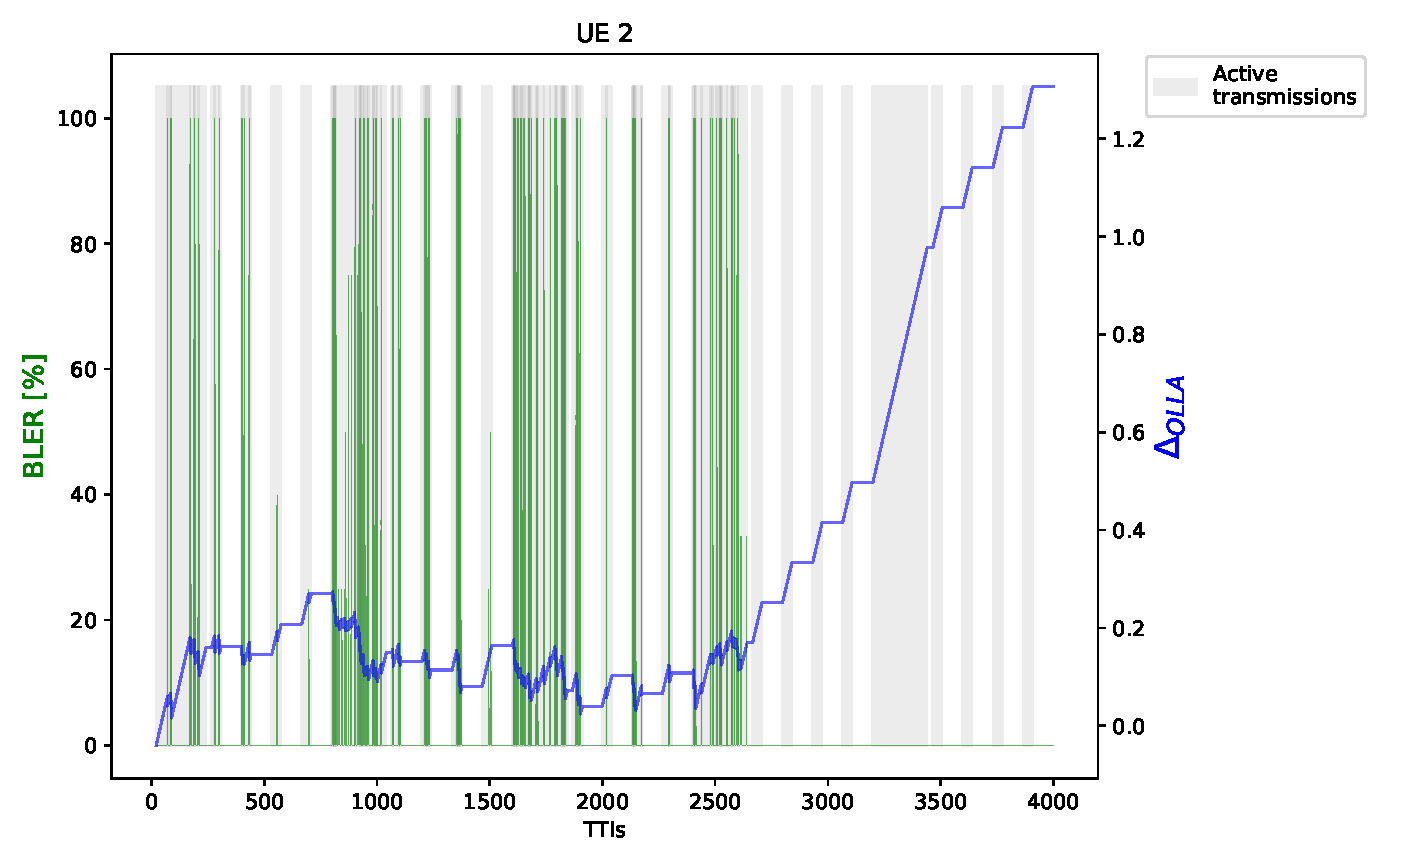
\includegraphics[scale = .6]{Results/mu_olla3.pdf}
    \captionsetup{type=figure} 
    \vspace{-3mm}   
    \caption{Link adaptation parameter variation with the instantaneous \acs{BLER}. Grey zones mark when the UE has active transmissions.}			
    \label{fig:mu_olla}
    
\end{center}

The use of this link adaptation scheme should make the BLER converge to the BLER target of 10\%. It still is uncertain why that does not happen and requires further investigation.

Finally, much like the previous section, we can derive some conclusions regarding how well the deployment and configurations cope with the requirements. However, it should not be taken as a final statement since some modelling simplifications listed in the beginning of this chapter were considered, some results are yet to be understood, and perhaps require rectifications, and this analysis lacks statistical significance: we cannot derive such conclusions by looking at one second of one use-case. But we can conclude something about that one second despite all limiting factors.

Nevertheless, to conclude something relevant we cannot resort exclusively to bit rate plots since those say nothing about performance with respect to latencies. From the application perspective, we want to answer questions such as: ``what is maximum application throughput that achieves less than X \% packet error rate?''

That is a difficult question, but we can take another sizeable step towards answering it, and also a step towards improving whatever that answer may be. That step consists in understanding in what circumstances the high packet loss occurs. 

Figure \ref{fig:mu_lat} shows the horizontal axis as frame indices instead of TTIs - they have a direct mapping: five GoP (each of duration 200 ms) are sent in one second, or 4000 TTIs. Furthermore, the I-frames have indices \{0, 6, 12, 18, 24\} and are marked in red. In the figure we can see the correlation between the average latency of packets belonging to the same frame and the packet drop rate for that frame. More importantly, we see as a general rule that both rise right after an I-frame.

\imagecapcontrol{Results/lat_drop_rate.pdf}{Packet latencies and drop-rates for all UEs with I-frame marking.}{fig:mu_lat}{.65}{-3mm}

We can notice that when packets are dropped, they are not dropped equally amongst all users - the percentage of dropped packets changes and the frame they belong to changes as well. If packets are dropped after the I frame, it means the link had enough quality to cope with the I frame, but having a P frame following with no pause led to the delay of some packets past the latency requirement. This is the case when the drop rate peak comes after the I-frame, which is the most common case. And the lower the drop rate peak is, the closer the user was to handling all packets within the required time. 

Another more extreme case is when the peak of the packet drop rate occurs during the I-frame transmission (e.g. the third I-frame of UE 0). This means that not all packets from that I-frame were sent within the latency budget.

Comparing Figures \ref{fig:mu_sinr} and \ref{fig:mu_lat} for UE 0 we see how the worst case in terms of packet average latency and drop rate clearly aligns with the worst experienced SINR across all users, at the 1500 TTI mark.

 \pagebreak
\section*{Conclusions}

This chapter objective was to validate the modelling framework.

In this chapter we started by defining the scenario as clearly as possible, as well as any simplifications that took place while simulating such scenario. We provided values to all variables we had previously defined in the Methodology Chapter.

Then, we assessed two reasons for rapid bit rate oscillations. One reason is when the number of packets arriving each TTI oscillates and the achieved bit rate is capped by the number of packets in the buffer. This happens when the channel is very good, which is the situation in Section \ref{sec:single-user}. And we have naturally concluded that we can only measure accurately what bit rate the link can achieve when the incoming packet bit rate surpasses the achievable bit rate.

The other possibility is when the channel is not optimal, to the point of causing some blocks to have errors, resulting in oscillations in the achieved bit rate. A mix case of phases with bit errors and phases with stable conditions is also possible, and often the case, which makes the situation harder to dissect and demands resorting to other metrics as well. Section \ref{sec:multi-user} was dedicated to exposing some of the metrics we can extract from simulations in order to assess these more complex situations. Also, the most important relations between metrics were put forth.

Although conclusions on radio layer configurations and deployment need to be done carefully given the light statistical evidence, we proved how they can be derived. For the scenario with multiple users, the requirements of 80 Mbps and 10 ms were only possible for UE 2, under the current setting. Actually, UE 2 supported such bit rate with sub-millisecond latencies. Next steps include expanding the quantity of acquired data from each simulation, longer simulations to enable correlation between events on a larger time scale, such as the head rotation, and altogether simulations on different channel realisations. 

Moreover, we have identified places that require further attention. Certainly some adjustments to the modelling and implementation are required to solve the few observed inconsistencies. Nonetheless, we have shown working simulations with predominantly coherent results. 





\cleardoublepage

%% %%%%%%%%%%%%%%%%%%%%%%%%%%%%%%%%%%%%%%%%%%%%%%%%%%%%%%%%%%%%%%%%%%%%%%
% Dummy Chapter:
% %%%%%%%%%%%%%%%%%%%%%%%%%%%%%%%%%%%%%%%%%%%%%%%%%%%%%%%%%%%%%%%%%%%%%%

% %%%%%%%%%%%%%%%%%%%%%%%%%%%%%%%%%%%%%%%%%%%%%%%%%%%%%%%%%%%%%%%%%%%%%%
% The Introduction:
% %%%%%%%%%%%%%%%%%%%%%%%%%%%%%%%%%%%%%%%%%%%%%%%%%%%%%%%%%%%%%%%%%%%%%%
\fancychapter{A Chapter}
\label{cap:chapter}

\textit{Present the chapter content.}

\section{Section A}
\label{sec:sectiona}

\subsection{Subsection A}
\label{subsec:subasectionA}

This would be a citation \cite{dummy}.

\ac{acro} 
% The first time you use this, the acronym will be written in full with the acronym in parentheses: supernova (SN). At later times it will just print the acronym: SN.

\acf{acro}
% written out form with acronym in parentheses, irrespective of previous use

\acs{acro}
% acronym form, irrespective of previous use

\acl{acro}
% written out form without following acronym

\acp{acro}
% plural form of acronym by adding an s. \acfp. \acsp, \aclp work as well.

As seen in \cite{wiki}. \emph{Enfatizar}

\subsection{Subsection B}
\label{subsec:subbsectiona}

\begin{figure}[H]
	\centering
		\includegraphics[width=0.5\linewidth]{2.Chapter/dummy.pdf}
	\caption[Dummy Figure Caption for List of Figures.]{Dummy Figure Caption.}
	\label{fig:dummyfigure1}
\end{figure}

Remember you can change the reference style. Another dummy citation \cite{sitedummy}.
\section{Section B}
\label{sec:sectionb}

\subsection{Subsection A}
\label{subsec:subasectionB}

The model described can also be represented as

\begin{equation}
\dot{\mathbf{x}}(t) = \mathbf{T}\mathbf{z}(y),\  \mathbf{y}(0) = \mathbf{y}_0,\  z\geq 0 \\
\label{eq:dummyeq1}
\end{equation}

\noindent where

\begin{equation}
\mathbf{A} = \left[ \begin{array}{cc} -(a_{12} + a_{10}) & a_{21} \\ a_{12} & -(a_{21} + a_{20}) \end{array} \right],\ \mathbf{x} = \left[ \begin{array}{c} x_1 \\ x_2 \end{array} \right] \\
\label{eq:dummyeq2}
\end{equation}


\subsection{Subsection B}
\label{subsec:subbsectionB}

\begin{table}[H]
	\centering
	\caption{Dummy Table.}
	\begin{tabular}{|c|c|c|c|} \hline
		\textbf{Vendor Name} 				& \textbf{Short Name}	& \textbf{Commercial Name}	& \textbf{Manufacturer}	\\ \hline \hline
		\multirow{3}{*}{Text in Multiple Row}		&	ABC				&  ABC\textreg				& ABC SA			         \\ \cline{2-4}
		 								&        DEF				&  DEF\textreg				& DEF SA				\\ \cline{2-4}
										&        GHF			&  GHF\textreg				& GHF SA				\\ \hline
		Text in Single Row					&        IJK				& IJK\textreg				& IJK SA				\\ \hline
		Frescos SA						&        LMN			& LMN\textreg				& LMN SA				\\ \hline
		Carros Lda.						&    \multicolumn{3}{|c|}{Text in Multiple Column}							\\ \hline
	\end{tabular}
	\label{tab:dummytable}
\end{table}
\cleardoublepage



%\fancychapter{Conclusion}
\label{cap:conclusion}


\section{Conclusions}


Something something concluding...

%\section*{Future Work}
%\label{sec:future-work}

% everything is in conclusions

\cleardoublepage
\cleardoublepage
% uncomment the next two lines to enable bibliography in the table of contents
%\phantomsection
%\addcontentsline{toc}{chapter}{Bibliography}
\bibliographystyle{myIEEEtran} % small change, see: tex.stackexchange.com/questions/87148/
\bibliography{biblio}
\cleardoublepage %this shouldn't be commented at the end

\begin{appendices}
	\begin{appendix}
		\pagenumbering{bychapter} 
        % appendix A
        \fancychapter{Deriving a Beam Steering Vector}
\label{sec:beam_steering}

This appendix shows how to obtain a convention beam steering vector, i.e. the vector of complex weights with unitary amplitudes and varying phases to multiply to each antenna element such that the beam has the desired direction. The derivation starts assuming the reader is familiar with antenna theory, and is knowledgeable about the principles behind beam steering. For a complete introduction antenna theory and beam-steering, consult \cite{balanis_antennas}. Additionally, we adapt the formulas with conventional references on the angles to better angular references that considerably facilitate computations with planar arrays.

Let us start by recalling that the radiation/antenna pattern of an antenna array is equal to its directivity scaled by the total radiation power. To facilitate comparisons, we will handle always the normalised version of the antenna pattern, i.e. its directivity. 

The directivity of the array $D_{array}$ for an uniform antenna array (same antenna elements, uniformly spaced) comes from the product of its current-normalised Array Factor $AF_n$ with the directivity of each antenna element $D_{ae}$. Equation \eqref{eq:d_arr} summarises this fact.

\begin{equation} \label{eq:d_arr}
    D_{array}(\phi, \theta) = \left|AF_n(\phi, \theta)\right|^2 \times D_{ae}(\phi, \theta)
\end{equation}

Furthermore, recall that conventional beam steering is nothing more than changing the array factor such that the resultant antenna pattern has a maximum along the intended direction. The array factor $AF$ with uniform element excitation and a setting illustrated in Figure \ref{fig:af_img} is given in Equation \eqref{eq:af}. Note that for the directivity we need the current-normalised version given by $AF_n = AF / I_0$.

\image{Appendix A/array figure.png}{Planar array geometry. From \cite{balanis_antennas}.}{fig:af_img}{.5}


\begin{align}
    AF(\phi, \theta) = I_0 \sum_{m=1}^{M} e^{j (m-1) \left(k d_x \cos(\phi)\sin(\theta) + \beta_x\right)} \sum_{n=1}^{N} e^{j (n-1) \left(k d_x \sin(\phi)\sin(\theta) + \beta_x\right)} \label{eq:af}
\end{align}


To maximise the power in a given direction we just have to change the phases differences $\beta_x$ and $\beta_y$ such that the exponentials equate 1, for any element/index of the sum. One does so by having the exponent be 0, by making the progressive phase shifts $\beta_x$ and $\beta_y$ be the symmetric of the other term in the same brackets. Consequently, creating a beam to $(\phi_0, \theta_0)$ implies having the progressive phase shifts like the left side of Equations \eqref{eq:phases1} and \eqref{eq:phases2}.

\begin{subequations}
    \begin{align}
        \beta_x &= -k d_x \cos(\phi_0) \sin(\theta_0) \label{eq:phases1} \\
        \beta_y &= -k d_y \sin(\phi_0) \sin(\theta_0) \label{eq:phases2}
    \end{align}
\end{subequations}


\subsection*{Angular Reference Adaptation}
When beam steering in a planar array, having choosing angular references appropriately can facilitate the computations down the line tremendously. As such, we define our new angular references in the array axis, i.e. the axis orthogonal to the plane where the array belongs. Assuming placing and antenna in the YoZ plane, the x axis would be the array axis. This is illustrated in Figure \ref{fig:newAngRef}.

\todo[inline]{Go to https://www.math10.com/en/geometry/geogebra/geogebra.html and draw how the planes are like and where the angles are. NOTE: THE REFERENCES ARE THE X AXIS (ARRAY AXIS) for the elevations and azimuth}

\image{Appendix A/newAngRef.jpg}{newAngRef}{fig:newAngRef}{.5}


Then we define relative azimuth $\phi_r$ and relative elevation $\theta_r$, also represented in figure \ref{fig:newAngRef}. Mathematically, $\phi_r = \phi$, but $\theta_r = 90 - \theta$. Therefore, in previous expressions, we transform $\sin(\theta) \rightarrow \cos(\theta_r)$. Note that this is the only change that $\beta_y$ goes through. Additionally, from the principles described in \cite{balanis_antennas}, we must now use $\beta_y$ and $\beta_z$ since there are phase increments along the y-axis and along the z-axis now.

In essence, this reference adaptation results in changes both in the $AF$ and in using different the progressive phase shifts $\beta_y$ and $\beta_z$. Since we require only the latter two to compute the steering vector the new progressive phase shifts are given in Equations \eqref{eq:new_phases1} and \eqref{eq:new_phases2}. 

\begin{subequations}
    \begin{align}
        \beta_y = -k d_x \sin({\phi_r}_0) \cos({\theta_r}_0) \label{eq:new_phases1} \\
        \beta_z = k d_y\cos({\phi_r}_0) \cos({\theta_r}_0)\label{eq:new_phases2}
    \end{align}
\end{subequations}

Note that this adaptation is beneficial not only to facilitate the mathematics for ourselves, but to better integrate our work with the formulations of the community since we could not find a formulation with the elevation and azimuth references along boresight. Such formulation should always be used in cases where the antenna physical orientation matters as it provides a solid base for computing gains based in relative directions. Additionally, this angular reference is widely used in software that performs this sort of computations, yet seldom explained.

For conciseness, the azimuth and elevation referred in the rest of the document are always the relative variants, but this will be reminded in the appropriate sections to avoid confusion.

Finally, to obtain the steering vector we follow a standard procedure, well explained in \cite{7925023}. We define incremental phase steps, along the y-axis denoted by $u_y$ and along the z-axis, denoted by $u_z$, and apply them to the antenna elements in given positions to coherently sum their contribution, see in Equation \eqref{eq:pmn}.
For the common inter-element spacing of half-wavelength in both orientations ($d_y = d_z = \lambda/2$), one may simplify the $\beta_y$ and $\beta_z$ as in Equations \eqref{eq:ux} and \eqref{eq:uy}.

\begin{align}
    p_{m,n} = u_z^{m-1} u_y^{n-1}, \ m &= 1, \dots, M, \label{eq:pmn} \\
    n &= 1, \dots, N \nonumber
\end{align}
\vspace{-1cm}


\begin{comment}
% WITHOUT RELATIVE AZIMUTH AND ELEVATION
\begin{align}
    u_x = e^{j \beta_x} &= e^{-j \pi \sin(\phi_0) \sin(\theta_0)} \label{eq:ux} \\
    u_y = e^{j \beta_y} &= e^{-j \pi \cos(\phi_0) \sin(\theta_0)} \label{eq:uy}
\end{align}
\end{comment}

\begin{align}
    u_y = e^{j \beta_y} &= e^{-j \pi \sin(\phi_r) \cos(\theta_r)} \label{eq:ux} \\
    u_z = e^{j \beta_z} &= e^{j \pi \cos(\phi_r) \cos(\theta_r)} \label{eq:uy}
\end{align}


And using \eqref{eq:pmn}, we obtain the precoding matrix in \eqref{eq:prec_mat}.

\begin{align} \label{eq:prec_mat}
    P = \begin{bmatrix}
        1 & \dots & u_y^{(N-1)}\\
        \vdots & \ddots & \vdots\\
        u_z^{(M-1)} &  & u_z^{(M-1)}u_y^{(N-1)}
        \end{bmatrix}
\end{align}

% Try to derive angles for antenna in the yOz plane, the same way they are derived for the xOy plane. use the 2 papers in this appendix
% Hopefully the result is what we say here to be.














 
        % appendix B
        
        %...
		\cleardoublepage
	\end{appendix}
\end{appendices}

\end{document}